\documentclass{Class/project_report}
\setTHSarabunFont
\usepackage{amssymb}
\usepackage{pifont}
\usepackage{enumitem}
\usepackage{float}
\geometry{a4paper,top=1.5in,bottom=1in,left=1.5in,right=1in}
\pagestyle{plain} % ตั้งค่า pagestyle เริ่มต้น
\newcolumntype{L}{>{\RaggedRight\arraybackslash}X} 
\newcolumntype{C}{>{\centering\arraybackslash}X}
\newcommand{\cmark}{\ensuremath{\checkmark}}
\newcommand{\xmark}{\ensuremath{\times}}
% Define full Thai alphabet for page numbering beyond 10
\makeatletter
\def\@thaialph#1{%
  \ifcase#1\or ก\or ข\or ค\or ง\or จ\or ฉ\or ช\or ซ\or ฌ\or ญ\or ฎ\or ฏ\or ฐ\or ฑ\or ฒ\or ณ\or ด\or ต\or ถ\or ท\or ธ\or น\or บ\or ป\or ผ\or ฝ\or พ\or ฟ\or ภ\or ม\or ย\or ร\or ล\or ว\or ศ\or ษ\or ส\or ห\or ฬ\or อ\or ฮ\else ?\fi
}
\def\thaialph#1{\expandafter\@thaialph\csname c@#1\endcsname}
\def\thaiAlph#1{\expandafter\@thaialph\csname c@#1\endcsname}
\makeatother

\begin{document}

    % Setup for Figures (centered label and text)
    \captionsetup[figure]{
      font={normalsize},
      labelfont={bold16pt},
      labelsep=quad,
      justification=centering,
      singlelinecheck=false,
      name={ภาพที่} % Add this line
    }
    % Setup for Tables (raggedright label and text)
    \captionsetup[table]{
      font={normalsize},
      labelfont={bold16pt},
      labelsep=quad,
      justification=raggedright,
      singlelinecheck=false,
      skip=8pt,
      indention=0.9in,
      name={ตารางที่} % Add this line
    }


    
    %*************************************
% ปกนอก
%*************************************
\newpage
\thispagestyle{empty}
\begin{center}

\vspace*{-0.8in}


\includegraphics[width=5.08cm]{Image/Logo_KMUTNB_Thai.png}
\vspace{2mm}

{\bf
    ปัญญาประดิษฐ์แชทบอทสำหรับองค์กร\\
    (กรณีศึกษา : บริษัท ฮาร์ทวอมมิ่ง จำกัด)
}

\vspace{0.3in}

\vspace{56mm}
\bf
นายวีรภัทร ชื่นชอบ\\  %ผู้จัดทำคนที่ 1
นายธนากร ธนบวรพล       %ผู้จัดทำคนที่ 2

\vspace{60mm}  

\vspace{0.4in}

{\bf 
    ปริญญานิพนธ์นี้เป็นส่วนหนึ่งของการศึกษาตามหลักสูตรวิทยาศาสตรบัณฑิต\\
    สาขาวิชาเทคโนโลยีสารสนเทศ ภาควิชาเทคโนโลยีสารสนเทศ\\
    คณะเทคโนโลยีและการจัดการอุตสาหกรรม มหาวิทยาลัยเทคโนโลยีพระจอมเกล้าพระนครเหนือ\\
    ปีการศึกษา 2569\\
    ลิขสิทธิ์ของมหาวิทยาลัยเทคโนโลยีพระจอมเกล้าพระนครเหนือ
}

\end{center}

%*************************************
% ปกในภาษาไทย
%*************************************
\newpage
\thispagestyle{empty}
\begin{center}

\vspace*{-0.5in}

{\bf
    ปัญญาประดิษฐ์แชทบอทสำหรับองค์กร
}

\vspace{0.1in}
{\bf
    (กรณีศึกษา : บริษัท ฮาร์ทวอมมิ่ง จำกัด)
}

\vspace{87mm}
\bf
นายวีรภัทร ชื่นชอบ\\    %ชื่อผู้จัดทำ1
นายธนากร ธนบวรพล       %ชื่อผู้จัดทำ2
\vspace{87mm}  

\vspace{0.1in}

{\bf
    ปริญญานิพนธ์นี้เป็นส่วนหนึ่งของการศึกษาตามหลักสูตรวิทยาศาสตรบัณฑิต\\
    สาขาวิชาเทคโนโลยีสารสนเทศ ภาควิชาเทคโนโลยีสารสนเทศ\\
    คณะเทคโนโลยีและการจัดการอุตสาหกรรม มหาวิทยาลัยเทคโนโลยีพระจอมเกล้าพระนครเหนือ\\
    ปีการศึกษา 2569\\
    ลิขสิทธิ์ของมหาวิทยาลัยเทคโนโลยีพระจอมเกล้าพระนครเหนือ
}

\end{center}

%*************************************
% ปกในภาษาอังกฤษ
%*************************************
\newpage
\thispagestyle{empty}
\begin{center}

\vspace*{-0.5in}

{\bf
    ARTIFICIAL INTELLIGENCE CHATBOT FOR ORGANIZATION
}

\vspace{0.2in}
{\bf
    (Case Study: Heartwarming Co., Ltd.)
}

\vspace{70mm}
\bf
MR. WEERAPHAT CHUENCHOB\\        %ชื่อผู้จัดทำ1
MR. THANAKORN THANABAWONPON        %ชื่อผู้จัดทำ2
\vspace{70mm}  

\vspace{0.2in}

{\bf
    PROJECT REPORT SUBMITTED IN PARTIAL FULFILLMENT OF THE REQUIREMENTS\\
    FOR THE BACHELOR’S DEGREE OF SCIENCE\\
    PROGRAM IN INFORMATION TECHNOLOGY\\
    DEPARTMENT OF INFORMATION TECHNOLOGY\\
    FACULTY OF INDUSTRIAL TECHNOLOGY AND MANAGEMENT\\
    KING MONGKUT’S UNIVERSITY OF TECHNOLOGY NORTH BANGKOK\\
    ACADEMIC YEAR 2026\\
    COPYRIGHT OF KING MONGKUT’S UNIVERSITY OF TECHNOLOGY NORTH BANGKOK
}

\end{center}


    
    %**************************************************************************************
% ใบรับรองโครงงาน กรณี ไม่มี ที่ปรึกษาร่วม
%**************************************************************************************
\newpage
\thispagestyle{empty}
\setstretch{1.25}
\setlength{\parindent}{0pt}

\vspace*{-0.5in}

\begin{tcolorbox}[colframe=black, colback=white, width=\textwidth, boxrule=0.8pt, arc=1mm, auto outer arc, left=10pt, right=10pt, top=10pt, bottom=10pt, enhanced jigsaw]

\begin{center}
\vspace{3mm}

\includegraphics[width=3.18cm]{Image/Logo_KMUTNB_Thai.png}

{\bf {\fontTwentyFour
    ใบรับรองปริญญานิพนธ์
    \\
}{\fontEighteen
    คณะเทคโนโลยีและการจัดการอุตสาหกรรม
    \\
    มหาวิทยาลัยเทคโนโลยีพระจอมเกล้าพระนครเหนือ
}}
\end{center}
\vspace{1em}
\fontSixTeen{
\begin{tabbing}
    เรื่อง  \= ปัญญาประดิษฐ์แชทบอทสำหรับองค์กร กรณีศึกษา ฮาร์ทวอมมิ่ง จำกัด       %ชื่อโปรเจ็คภาษาไทย
    \\
    โดย  \> นายวีรภัทร ชื่นชอบ     %ชื่อผู้จัดทำ1 
    \\     %เว้นบรรทัด เมื่อมีเพื่อนร่วมโปรเจ็ค
        \> นายธนากร ธนบวรพล       %ชื่อผู้จัดทำ2
    \\
    \\
         \> ได้รับอนุมัติให้นับเป็นส่วนหนึ่งของการศึกษาตาม 
    \\
         \> หลักสูตรวิทยาศาสตรบัณฑิต  สาขาวิชาเทคโนโลยีสารสนเทศ ภาควิชาเทคโนโลยีสารสนเทศ
\end{tabbing}

\vspace{1.5em}

\begin{flushright}
\makebox[8cm][l]{\rule{7cm}{0.4pt} คณบดี} \\
\makebox[8cm][l]{(ผู้ช่วยศาสตราจารย์ ดร.กฤษฎากร  บุดดาจันทร์)}
\end{flushright}

\vspace{8mm}

\vspace{0.2in}

คณะกรรมการสอบปริญญานิพนธ์

\vspace{1.5em}
\begin{flushleft}
\makebox[7cm][l]{\rule{7cm}{0.4pt} ประธานกรรมการ} \\
\makebox[7cm][c]{(ผู้ช่วยศาสตราจารย์ ดร.สุปิติ กุลจันทร์)}       %ระบุชื่อประธานกรรมการ
\end{flushleft}

\vspace{1.5em}
\begin{flushleft}
\makebox[7cm][l]{\rule{7cm}{0.4pt} กรรมการ} \\
\makebox[7cm][c]{(ผู้ช่วยศาสตราจารย์ ดร.พาฝัน ดวงไพศาล)}            %ระบุชื่อกรรมการ
\end{flushleft}

\vspace{1.5em}
\begin{flushleft}
\makebox[7cm][l]{\rule{7cm}{0.4pt} อาจารย์ที่ปรึกษา} \\
\makebox[7cm][c]{(อาจารย์ ดร.ศิรินทรา แว่วศรี)}       %ระบุชื่ออาจารย์ที่ปรึกษาโปรเจ็ค
\end{flushleft}

} %end fontSixTeen
\end{tcolorbox}
 % กรณีไม่มีที่ปรึกษาร่วม (เลือกใบรับรองเพียงใบเดียว)
    % %**************************************************************************************
% ใบรับรองโครงงาน กรณี มี ที่ปรึกษาร่วม
%**************************************************************************************
\newpage
\thispagestyle{empty}
\setstretch{1.25}
\setlength{\parindent}{0pt}

\begin{tcolorbox}[colframe=black, colback=white, width=\textwidth, boxrule=0.8pt, arc=1mm, auto outer arc, left=10pt, right=10pt, top=10pt, bottom=10pt, enhanced jigsaw]

\begin{center}
\vspace{3mm}

\includegraphics[width=3.18cm]{Image/Logo_KMUTNB_Thai.png}

{\bf {\fontTwentyFour
    ใบรับรองปริญญานิพนธ์
    \\
}{\fontEighteen
    คณะเทคโนโลยีและการจัดการอุตสาหกรรม
    \\
    มหาวิทยาลัยเทคโนโลยีพระจอมเกล้าพระนครเหนือ
}}
\end{center}
\vspace{1em}
\fontSixTeen{
\begin{tabbing}
    เรื่อง  \= ปัญญาประดิษฐ์แชทบอทสำหรับองค์กร กรณีศึกษา ฮาร์ทวอมมิ่ง จำกัด       %ชื่อโปรเจ็คภาษาไทย
    \\
    โดย  \> นายวีรภัทร ชื่นชอบ     %ชื่อผู้จัดทำ1 
    \\     %เว้นบรรทัด เมื่อมีเพื่อนร่วมโปรเจ็ค
        \> นายธนากร ธนบวรพล       %ชื่อผู้จัดทำ2
    \\
    \\
         \> ได้รับอนุมัติให้นับเป็นส่วนหนึ่งของการศึกษาตาม 
    \\
         \> หลักสูตรวิทยาศาสตรบัณฑิต  สาขาวิชาเทคโนโลยีสารสนเทศ ภาควิชาเทคโนโลยีสารสนเทศ
\end{tabbing}

\vspace{1em}

\begin{flushright}
\makebox[8cm][l]{\rule{7cm}{0.4pt} คณบดี} \\
\makebox[8cm][l]{(ผู้ช่วยศาสตราจารย์ ดร.กฤษฎากร  บุดดาจันทร์)}
\end{flushright}

\vspace{0.9em}

คณะกรรมการสอบปริญญานิพนธ์

\vspace{0.9em}
\begin{flushleft}
\makebox[7cm][l]{\rule{7cm}{0.4pt} ประธานกรรมการ} \\
\makebox[7cm][c]{(ผู้ช่วยศาสตราจารย์ ดร.สุปิติ กุลจันทร์)}       %ระบุชื่อประธานกรรมการ
\end{flushleft}

\vspace{0.9em}
\begin{flushleft}
\makebox[7cm][l]{\rule{7cm}{0.4pt} กรรมการ} \\
\makebox[7cm][c]{(ผู้ช่วยศาสตราจารย์ ดร.พาฝัน ดวงไพศาล)}            %ระบุชื่อกรรมการ
\end{flushleft}

\vspace{0.9em}
\begin{flushleft}
\makebox[7cm][l]{\rule{7cm}{0.4pt} อาจารย์ที่ปรึกษา} \\
\makebox[7cm][c]{(อาจารย์ ดร.ศิรินทรา แว่วศรี)}       %ระบุชื่ออาจารย์ที่ปรึกษาโปรเจ็ค
\end{flushleft}

} %end fontSixTeen
\end{tcolorbox}
 % กรณีมีที่ปรึกษาร่วม

    
    \newpage
    \thaiPageStyle
    \setcounter{page}{2}
    \fontSixTeen
    \justifying
    %**************************************************************************************
% บทคัดย่อภาษาไทย
%**************************************************************************************
\phantomsection
\addcontentsline{toc}{chapter}{บทคัดย่อภาษาไทย}

\vspace*{-0.85in}

{\renewcommand{\arraystretch}{0.75}
\begin{tabularx}{\textwidth}{l L}
ชื่อ                           & : นายวีรภัทร ชื่นชอบ\\
                             & : นายธนากร ธนบวรพล\\
ชื่อปริญญานิพนธ์                  & : ปัญญาประดิษฐ์แชทบอทสำหรับองค์กร กรณีศึกษา ฮาร์ทวอมมิ่ง จำกัด\\
สาขาวิชา                       & : เทคโนโลยีสารสนเทศ\\
สถาบัน                         & : มหาวิทยาลัยเทคโนโลยีพระจอมเกล้าพระนครเหนือ\\
อาจารย์ที่ปรึกษาปริญญานิพนธ์        & : อาจารย์ ดร.ศิรินทรา แว่วศรี\\
ปีการศึกษา                     & : 2569\\
\end{tabularx}
}

\vspace{-2mm}
\begin{center}\textbf{บทคัดย่อ}\end{center}
\vspace{-3mm}

\hspace*{1.5em}ปริญญานิพนธ์นี้มีวัตถุประสงค์เพื่อวิเคราะห์ ออกแบบ และพัฒนาระบบปัญญาประดิษฐ์แชทบอทสำหรับองค์กร กรณีศึกษา บริษัท ฮาร์ทวอมมิ่ง จำกัด ผู้นำเข้าและจัดจำหน่ายสินค้าไลฟ์สไตล์พรีเมียม โดยนำเทคโนโลยีปัญญาประดิษฐ์มาแก้ไขปัญหาข้อมูลกระจัดกระจาย ความล่าช้าในการสืบค้นข้อมูลสินค้าและระเบียบปฏิบัติ ความผิดพลาดในการบันทึกบัญชีรายรับ-รายจ่ายจากสลิปโอนเงินและใบเสร็จ ตลอดจนความยุ่งยากในการบริหารงานบุคคล เช่น การยื่นใบลาและการอนุมัติงาน

\hspace*{1.5em}ระบบที่พัฒนาขึ้นผสานการทำงานของ LINE Official Account ผ่าน LINE Messaging API ร่วมกับเว็บแอปพลิเคชันส่วนกลาง พัฒนาด้วย Python Flask, SQLite และ ChromaDB โดยในภาคการศึกษาที่ 1/2569 ได้ดำเนินการวิเคราะห์ ออกแบบระบบ และพัฒนาระบบส่วนโครงสร้างพื้นฐาน ได้แก่ 1) ระบบยืนยันตัวตนและจัดการบัญชีผู้ใช้งาน (Email/Password, Google OAuth 2.0, LINE Linking) 2) ระบบคลังความรู้อัจฉริยะ (RAG) เชื่อมต่อโมเดลภาษาขนาดใหญ่ Google Gemini เพื่อสืบค้นและตอบคำถามภาษาธรรมชาติจากเอกสารองค์กร (PDF, TXT, สเปรดชีต) 3) ระบบค้นหาเวกเตอร์ (Vector Search) ด้วย ChromaDB และ FastEmbed และ 4) ระบบจัดการเอกสารเชื่อมโยง Google Drive จัดระเบียบไฟล์แยกโฟลเดอร์อัตโนมัติ

\hspace*{1.5em}ผลการดำเนินงานในภาคการศึกษาที่ 1/2569 พบว่า ระบบโครงสร้างพื้นฐานและโมเดลคลังความรู้ที่พัฒนาขึ้นสามารถทำงานได้ครบถ้วนตามขอบเขตที่กำหนด โดยผ่านการทดสอบการทำงานเบื้องต้น (Black-Box Testing) ระบบสามารถรับข้อความคำถามผ่าน LINE Official Account และประมวลผลดึงคำตอบจากเอกสารของบริษัทมาตอบกลับในรูปแบบ Flex Message ได้อย่างถูกต้องและตรงตามบริบทของสินค้าจริง สำหรับระบบจัดการการเงินและบัญชีอัตโนมัติด้วยเทคโนโลยี OCR, ระบบบริหารงานบุคคล, แผงควบคุมสถิติภาพรวม และการประเมินความพึงพอใจของผู้ใช้งานจริง จะดำเนินการพัฒนาและประเมินผลในภาคการศึกษาที่ 2/2569 ต่อไป

\vspace{1mm}
\begin{flushright}
(ปริญญานิพนธ์มีจำนวนทั้งสิ้น \pageref{LastPage} หน้า)

\vspace{2mm}
\rule{8 cm}{0.4pt} อาจารย์ที่ปรึกษาปริญญานิพนธ์\\
(อาจารย์ ดร.ศิรินทรา แว่วศรี)
\end{flushright}


%**************************************************************************************
% บทคัดย่อภาษาอังกฤษ
%**************************************************************************************
\newpage
\phantomsection
\addcontentsline{toc}{chapter}{บทคัดย่อภาษาอังกฤษ}

\vspace*{-0.85in}

{\renewcommand{\arraystretch}{0.75}
\begin{tabularx}{\textwidth}{l L}
Name                    & : MR. WEERAPHAT CHUENCHOB\\
                        & : MR. THANAKORN THANABAWONPON\\
Project Title           & : Artificial Intelligence Chatbot for Organization (Case Study: Heartwarming Co., Ltd.)\\
Major Field             & : Information Technology\\
Institution             & : King Mongkut’s University of Technology North Bangkok\\
Project Advisor         & : Dr. Sirintra Vaiwsri\\
Academic Year           & : 2026\\
\end{tabularx}
}

\vspace{-2mm}
\begin{center}\textbf{Abstract}\end{center}
\vspace{-3mm}

\hspace*{1.5em}The objective of this special project is to analyze, design, and develop an Artificial Intelligence Chatbot for Organization, with Heartwarming Company Limited as a case study. The project applies artificial intelligence technologies to address problems regarding scattered enterprise information, delayed product inquiries, manual bookkeeping errors from transaction slips and invoices, and cumbersome human resource management processes such as leave requests and approvals.

\hspace*{1.5em}The system integrates LINE Official Account via LINE Messaging API with a centralized web dashboard, engineered using Python Flask, SQLite, and ChromaDB. In the first semester of academic year 2026 (Semester 1/2026), the project focuses on infrastructure analysis, system design, and core module implementation, comprising: 1) user management and authentication (Email/Password, Google OAuth 2.0, LINE Linking), 2) Retrieval-Augmented Generation (RAG) knowledge base leveraging Google Gemini to answer natural language questions from company documents (PDF, TXT, Spreadsheets), 3) semantic vector search utilizing ChromaDB and FastEmbed, and 4) document management integrated with Google Drive API for automated folder organization.

\hspace*{1.5em}The implementation results for Semester 1/2026 demonstrate that all planned core infrastructure modules operate successfully according to defined specifications, verified through baseline Black-Box testing. The chatbot seamlessly handles incoming queries via LINE OA and synthesizes accurate, context-aware responses presented via interactive LINE Flex Messages. The advanced automated financial bookkeeping with OCR, human resource leave management, executive analytical dashboard, and formal end-user satisfaction evaluation will be subsequently implemented and evaluated in Semester 2/2026.

\vspace{1mm}
\begin{flushright}
(Total \pageref{LastPage} pages)

\vspace{2mm}
\rule{8 cm}{0.4pt} Project Advisor\\
(Dr. Sirintra Vaiwsri)
\end{flushright}


%**************************************************************************************
% กิตติกรรมประกาศ
%**************************************************************************************
\newpage
\phantomsection
\addcontentsline{toc}{chapter}{กิตติกรรมประกาศ}

\vspace*{-0.5in}

\begin{center}\textbf{กิตติกรรมประกาศ}\end{center}
\vspace*{0.2in}

\hspace*{1.5em}ปริญญานิพนธ์ เรื่อง "ปัญญาประดิษฐ์แชทบอทสำหรับองค์กร กรณีศึกษา ฮาร์ทวอมมิ่ง จำกัด" ฉบับนี้ สำเร็จลุล่วงไปได้ด้วยความกรุณาและความช่วยเหลืออย่างดียิ่งจาก อาจารย์ ดร.ศิรินทรา แว่วศรี อาจารย์ที่ปรึกษาปริญญานิพนธ์ ที่ได้กรุณาสละเวลาให้คำปรึกษา แนะนำแนวทางการวิเคราะห์ ออกแบบระบบ และการแก้ไขปัญหาทางเทคนิคต่าง ๆ ตลอดจนตรวจสอบและปรับปรุงรายงานฉบับนี้ให้มีความถูกต้องสมบูรณ์ คณะผู้จัดทำขอกราบขอบพระคุณเป็นอย่างสูงไว้ ณ โอกาสนี้

\vspace{0.8em}
\hspace*{1.5em}ขอขอบพระคุณ ผู้ช่วยศาสตราจารย์ ดร.สุปิติ กุลจันทร์ ประธานกรรมการสอบปริญญานิพนธ์ และผู้ช่วยศาสตราจารย์ ดร.พาฝัน ดวงไพศาล กรรมการสอบปริญญานิพนธ์ ที่ได้ให้ข้อเสนอแนะเชิงวิชาการอันทรงคุณค่า เพื่อให้โครงงานมีความสมบูรณ์รอบด้านยิ่งขึ้น

\vspace{0.8em}
\hspace*{1.5em}ขอขอบพระคุณ ผู้บริหารและพนักงานของ บริษัท ฮาร์ทวอมมิ่ง จำกัด ทุกท่าน ที่ได้ให้ความอนุเคราะห์ข้อมูลจริงในการศึกษา ให้ความร่วมมือในการทดสอบระบบ และให้ข้อเสนอแนะจากการใช้งานจริง ซึ่งเป็นประโยชน์อย่างยิ่งต่อการพัฒนาระบบให้ตอบสนองความต้องการของธุรกิจได้อย่างแท้จริง

\vspace{0.8em}
\hspace*{1.5em}ท้ายที่สุดนี้ คณะผู้จัดทำขอกราบขอบพระคุณ บิดา มารดา และครอบครัว ที่ได้ให้การอุปการะสนับสนุนการศึกษา และเป็นกำลังใจสำคัญเสมอมา ตลอดจนเพื่อน ๆ นักศึกษาสาขาวิชาเทคโนโลยีสารสนเทศ ที่ได้แลกเปลี่ยนความรู้และให้ความช่วยเหลือตลอดระยะเวลาการศึกษา

\vspace{1.5cm}
\begin{flushright}
นายวีรภัทร ชื่นชอบ\\
นายธนากร ธนบวรพล
\end{flushright}

    \newgeometry{a4paper,top=1.5in,bottom=1in,left=1.5in,right=1in,includehead}
    \setTHSarabunFont
    \fontsize{16}{16}\selectfont
    \thaiPageStyle
    \customTOCthai
    \newpage
    \customLOFthai
    \newpage
    \begingroup
    \linespread{0.93}\selectfont
    \fancyhead[C]{\textbf{สารบัญตาราง (ต่อ)}\\[4pt]\textbf{ตารางที่}\hfill\textbf{หน้า}}
    \customLOTthai
    \endgroup
    \clearpage % ขึ้นหน้าใหม่หลังจากหน้าที่มีการปรับ margin
    \restoregeometry % คืนค่า geometry กลับเป็นค่าเริ่มต้น
    \fancyhf{} % ล้างการตั้งค่า fancyhdr ของหน้าที่ปรับ
    \setTHSarabunFont
    \fontsize{16}{16}\selectfont
    \thaiPageStyle
    
    \newpage
    \setlength{\headheight}{0cm}
    \setcounter{page}{1}
    \arabicPageTopRight % ตั้งค่าต่อไปใช้สไตล์อารบิกมุมขวาบน
    \customTOCarabic
    %*************************************
% บทที่ 1
%*************************************
\chapterTitle{1}{บทนำ}

% คำสั่งสำหรับจัดรายการหัวข้อย่อยแบบชิดสวยงาม ไม่มีช่องว่างกว้างผิดปกติ
\providecommand{\decitem}[2]{%
  \par\noindent\hangindent=3.6em\hangafter=1\hspace*{1.3em}#1\hspace{0.5em}#2\par\vspace{0.25em}%
}
\providecommand{\subdecitem}[2]{%
  \par\noindent\hangindent=5.8em\hangafter=1\hspace*{2.0em}#1\hspace{0.5em}#2\par\vspace{0.22em}%
}

\section{ความเป็นมาและความสำคัญของปัญหา}
\hspace*{1.3em}
ในยุคเศรษฐกิจดิจิทัลปัจจุบัน องค์กรธุรกิจขนาดเล็กและขนาดกลาง (Small and Medium Enterprises: SMEs) มีบทบาทสำคัญอย่างยิ่งต่อการขับเคลื่อนเศรษฐกิจของประเทศ อย่างไรก็ดี องค์กรขนาดเล็กถึงขนาดกลางมักเผชิญกับข้อจำกัดด้านทรัพยากรบุคคล งบประมาณ และเครื่องมือทางเทคโนโลยีที่ใช้ในการบริหารจัดการข้อมูล การดำเนินงานส่วนใหญ่ยังคงพึ่งพาการทำงานแบบดั้งเดิม (Manual Process) เช่น การบันทึกบัญชีลงสมุด การจดบันทึกเอกสารลงสเปรดชีตที่กระจัดกระจายตามเครื่องของพนักงานแต่ละคน และการประสานงานผ่านแอปพลิเคชันสนทนาที่ไม่มีการจัดหมวดหมู่อย่างเป็นระบบ ส่งผลให้เกิดปัญหาข้อมูลสูญหาย การสื่อสารคลาดเคลื่อน และความล่าช้าในการดำเนินธุรกิจ

\hspace*{1.3em}
กรณีศึกษา บริษัท ฮาร์ทวอมมิ่ง จำกัด ซึ่งเป็นผู้นำเข้าและตัวแทนจัดจำหน่ายสินค้าไลฟ์สไตล์พรีเมียมจากต่างประเทศอย่างเป็นทางการในประเทศไทย ได้แก่ แบรนด์ "duit" ผลิตภัณฑ์นวัตกรรมของใช้และเฟอร์นิเจอร์สัตว์เลี้ยงดีไซน์มินิมอล เช่น เครื่องให้อาหารอัตโนมัติ น้ำพุสัตว์เลี้ยง และกระบะทรายอัจฉริยะ, แบรนด์ "thumb toe" ถุงเท้าพิลาทิสและถุงเท้าแฟชั่นออกกำลังกายที่เน้นการทรงตัว และแบรนด์ "by.tuneteller" ฟองน้ำแต่งหน้าแบบตบแห้งคุณภาพสูง โดยมีช่องทางการจัดจำหน่ายหลักผ่านแพลตฟอร์มอีคอมเมิร์ซและมาร์เก็ตเพลสชั้นนำ ได้แก่ Shopee, Lazada, TikTok Shop และ LINE Official Account (LINE OA) ควบคู่กับการออกบูธแสดงสินค้าในงานนิทรรศการต่าง ๆ เพื่อสร้างการรับรู้แบรนด์

\hspace*{1.3em}
จากการศึกษาและวิเคราะห์กระบวนการทำงานจริงภายใน บริษัท ฮาร์ทวอมมิ่ง จำกัด พบว่าองค์กรกำลังเผชิญกับปัญหาสำคัญในการดำเนินงาน 4 ประการหลัก ดังนี้:

\vspace{0.2em}
\noindent\hspace*{1.3em}\textbf{1) ปัญหาการค้นหาข้อมูลและเอกสารองค์กร:} ข้อมูลรายละเอียดสินค้า คุณสมบัติ คู่มือการใช้งาน นโยบายการรับประกันสินค้า ระเบียบการปฏิบัติงาน และคำถามที่พบบ่อย (FAQ) ถูกจัดเก็บแยกย่อยในเอกสารไฟล์ PDF, ข้อความ และสเปรดชีตหลายแหล่ง เมื่อพนักงานต้องการสืบค้นข้อมูลเพื่อตอบคำถามลูกค้าหรือแก้ไขปัญหาหน้างาน ต้องใช้เวลาค้นหานานและบ่อยครั้งที่พนักงานใหม่ให้ข้อมูลแก่ลูกค้าไม่ถูกต้องตรงกัน\par\vspace{0.3em}

\noindent\hspace*{1.3em}\textbf{2) ปัญหาความผิดพลาดและความล่าช้าในการทำบัญชีรายรับ-รายจ่าย:} ในแต่ละวันมีรายการรับเงินและจ่ายเงินผ่านช่องทางออนไลน์จำนวนมาก พนักงานต้องรวบรวมภาพถ่ายใบเสร็จรับเงิน ใบกำกับภาษี และสลิปการโอนเงินของลูกค้าและซัพพลายเออร์ จากนั้นต้องพิมพ์กรอกตัวเลขและรายละเอียดลงในสมุดบัญชีด้วยมือ (Manual Data Entry) ซึ่งใช้เวลามาก เกิดความผิดพลาดของตัวเลข และเกิดความล่าช้าในการสรุปงบการเงินประจำเดือน\par\vspace{0.3em}

\noindent\hspace*{1.3em}\textbf{3) ปัญหาการบริหารงานบุคคลที่ขาดระบบศูนย์กลาง:} การยื่นคำขอลางานของพนักงาน เช่น ลาป่วย ลากิจ ลาพักร้อน ยังใช้วิธีการส่งข้อความส่วนตัวหรือกระดาษ ทำให้หัวหน้างานตรวจสอบประวัติการลาและคำนวณโควตาวันลาคงเหลือได้ยาก ข้อมูลการขาด ลา มาสาย มักตกหล่นและเกิดความสับสนในการบันทึกสถิติการทำงาน\par\vspace{0.3em}

\noindent\hspace*{1.3em}\textbf{4) ปัญหาความยุ่งยากจากการสลับใช้งานหลายซอฟต์แวร์ (App Fatigue):} พนักงานต้องสลับการทำงานไปมาระหว่างหลายแอปพลิเคชัน เช่น โปรแกรมแชทสำหรับคุยกับลูกค้า สเปรดชีตสำหรับเช็คสต็อก โฟลเดอร์รวมสลิปการเงิน และแอปพลิเคชันสำหรับยื่นใบลา ซึ่งนอกจากจะสร้างความยุ่งยากในการเรียนรู้ระบบแล้ว การจัดซื้อซอฟต์แวร์สำเร็จรูปหลายตัวยังมีค่าบริการรายเดือนที่สูงเกินไปสำหรับธุรกิจ SME\par\vspace{0.4em}

\hspace*{1.3em}
จากสภาพปัญหาดังกล่าว คณะผู้จัดทำจึงได้เล็งเห็นถึงโอกาสในการนำเทคโนโลยีปัญญาประดิษฐ์ (Artificial Intelligence: AI) และโมเดลภาษาขนาดใหญ่ (Large Language Models: LLM) มาบูรณาการร่วมกับแพลตฟอร์ม LINE ซึ่งเป็นแอปพลิเคชันสนทนาที่พนักงานในประเทศไทยมีความคุ้นเคยและใช้งานเป็นประจำอยู่แล้ว ผ่านเทคโนโลยี LINE Messaging API ร่วมกับการพัฒนาเว็บแอปพลิเคชันบริหารจัดการส่วนกลาง (Centralized Web Dashboard) โดยประยุกต์ใช้เทคนิคการค้นคืนข้อมูลเสริมด้วยปัญญาประดิษฐ์ (Retrieval-Augmented Generation: RAG) เพื่อสร้างระบบคลังความรู้อัจฉริยะที่สามารถสืบค้นคำตอบจากเอกสารของบริษัทได้อย่างแม่นยำ ผสานกับเทคโนโลยีการรู้จำอักขระด้วยแสง (Optical Character Recognition: OCR) ในการอ่านและสกัดข้อมูลจากภาพถ่ายสลิปโอนเงินและใบเสร็จ แล้วนำไปลงบัญชีใน Google Sheets พร้อมจัดเก็บเอกสารลง Google Drive ให้อัตโนมัติ ตลอดจนพัฒนาระบบบริหารงานบุคคลสำหรับการขอลางานผ่าน LINE ได้อย่างสะดวกรวดเร็ว

\hspace*{1.3em}
การพัฒนาระบบปัญญาประดิษฐ์แชทบอทสำหรับองค์กรนี้ จึงไม่เพียงแต่ช่วยลดขั้นตอนและระยะเวลาในการทำงานของพนักงาน แต่ยังช่วยลดข้อผิดพลาดในการลงบัญชี เพิ่มความคล่องตัวในการดำเนินธุรกิจ และช่วยให้ผู้บริหารมีข้อมูลสารสนเทศที่ถูกต้อง ครบถ้วน เพื่อนำไปใช้ประกอบการตัดสินใจทางธุรกิจได้อย่างมีประสิทธิภาพและคุ้มค่าต่อการลงทุน

\section{วัตถุประสงค์ของการจัดทำโครงงานพิเศษ}
\hspace*{1.3em}
การจัดทำโครงงานพิเศษนี้ มีวัตถุประสงค์หลัก 5 ประการ ดังนี้:

\vspace{0.2em}
\decitem{1.2.1}{เพื่อวิเคราะห์ ออกแบบ และพัฒนาระบบแชทบอทอัจฉริยะที่ทำงานผ่านแพลตฟอร์ม LINE Official Account ร่วมกับเว็บแอปพลิเคชัน สำหรับช่วยเหลืองานและบริหารจัดการภายในองค์กร}

\decitem{1.2.2}{เพื่อประยุกต์ใช้เทคโนโลยีปัญญาประดิษฐ์ในการสร้างระบบคลังความรู้อัจฉริยะ (Retrieval-Augmented Generation: RAG) ที่สามารถค้นหาคำตอบและดึงข้อมูลจากเอกสารองค์กรได้อย่างถูกต้องและอัตโนมัติ}

\decitem{1.2.3}{เพื่อพัฒนาระบบจัดการการเงินและบัญชีที่ใช้เทคโนโลยี OCR ในการอ่านข้อมูลจากใบเสร็จรับเงินและสลิปโอนเงิน แล้วนำข้อมูลไปบันทึกลงบัญชีใน Google Sheets พร้อมจัดเก็บไฟล์บน Google Drive โดยอัตโนมัติ}

\decitem{1.2.4}{เพื่อพัฒนาระบบบริหารงานบุคคลเบื้องต้น เช่น ระบบการยื่นคำขอลางาน ระบบการอนุมัติใบลาผ่านช่องทาง LINE และระบบตรวจสอบสิทธิ์วันลาคงเหลือของพนักงาน}

\decitem{1.2.5}{เพื่อพัฒนาเว็บแอปพลิเคชันสำหรับผู้ดูแลระบบ (Admin Web Dashboard) ที่แสดงผลสรุปภาพรวมการดำเนินงานขององค์กร การจัดการผู้ใช้งาน การควบคุมสิทธิ์ตามบทบาท (RBAC) และบันทึกประวัติการทำงานของระบบได้อย่างครบถ้วน}

\section{ขอบเขตของการทำโครงงานพิเศษ} \label{sec1:scope}
\hspace*{1.3em}
การดำเนินงานจัดทำโครงงานพิเศษ แบ่งการดำเนินงานออกเป็น 2 ภาคการศึกษา โดยมีขอบเขตของระบบครอบคลุมรายละเอียดดังนี้:

\subsection{ภาคการศึกษาที่ 1}
\hspace*{1.3em}
โครงสร้างพื้นฐานระบบจัดการผู้ใช้ ระบบสมาชิก คลังความรู้ RAG และการจัดการไฟล์

\vspace{0.4em}
\noindent\hspace*{1.3em}\textbf{1.3.1.1 ด้านระบบจัดการผู้ใช้งาน (User Management)}\par\nopagebreak\vspace{0.25em}
\subdecitem{1.3.1.1.1}{สมัครสมาชิกและยืนยันตัวตนเข้าสู่ระบบผ่านอีเมลและรหัสผ่าน (Email \& Password Authentication)}
\subdecitem{1.3.1.1.2}{เข้าสู่ระบบผ่านบัญชี LINE (LINE Login OAuth 2.0) และบัญชี Google (Google OAuth 2.0)}
\subdecitem{1.3.1.1.3}{มีระบบจัดการข้อมูลโปรไฟล์ส่วนตัวของผู้ใช้งาน การแก้ไขรหัสผ่าน และการกู้คืนรหัสผ่านด้วย OTP}
\subdecitem{1.3.1.1.4}{มีระบบควบคุมความปลอดภัยของเซสชัน (Session Management) และตรวจสอบสถานะการเข้าสู่ระบบ}

\vspace{0.4em}
\noindent\hspace*{1.3em}\textbf{1.3.1.2 ด้านระบบแชทบอทอัจฉริยะและคลังความรู้ (AI Chatbot \& Knowledge Base)}\par\nopagebreak\vspace{0.25em}
\subdecitem{1.3.1.2.1}{เชื่อมต่อระบบแชทบอทกับบัญชี LINE Official Account ขององค์กรผ่าน LINE Messaging API}
\subdecitem{1.3.1.2.2}{ระบบคลังความรู้อัจฉริยะ (RAG System) ที่รองรับการอัปโหลดไฟล์เอกสารองค์กร ได้แก่ PDF, DOCX, TXT และสเปรดชีต}
\subdecitem{1.3.1.2.3}{ระบบแปลงเอกสารเป็นเวกเตอร์เอ็มเบดดิง (Vector Embeddings) และจัดเก็บในฐานข้อมูลเวกเตอร์ ChromaDB}
\subdecitem{1.3.1.2.4}{ระบบสืบค้นข้อมูลตามบริบทความหมาย (Semantic Similarity Search) เพื่อดึงข้อความที่เกี่ยวข้องมาสร้างคำตอบด้วยโมเดลภาษาขนาดใหญ่ Google Gemini}

\vspace{0.4em}
\noindent\hspace*{1.3em}\textbf{1.3.1.3 ด้านระบบจัดการเอกสารองค์กร (Document Management)}\par\nopagebreak\vspace{0.25em}
\subdecitem{1.3.1.3.1}{รองรับการอัปโหลดไฟล์หลายรูปแบบผ่านหน้าเว็บและช่องแชท LINE}
\subdecitem{1.3.1.3.2}{เชื่อมต่อกับบริการคลาวด์ Google Drive API เพื่อจัดระเบียบไฟล์แยกโฟลเดอร์ตามวันที่และหมวดหมู่อัตโนมัติ}
\subdecitem{1.3.1.3.3}{รองรับการสืบค้นและดึงลิงก์ไฟล์ย้อนหลังผ่านคำสั่งในช่องแชท LINE}

\vspace{0.4em}
\noindent\hspace*{1.3em}\textbf{1.3.1.4 ด้านระบบเชื่อมต่อแพลตฟอร์ม LINE (LINE Platform Integration)}\par\nopagebreak\vspace{0.25em}
\subdecitem{1.3.1.4.1}{พัฒนาเว็บฮุก (Webhook Handler) สำหรับรับส่งข้อความ เหตุการณ์ และมัลติมีเดีย (รูปภาพ, เอกสาร, พิกัดตำแหน่ง) อัตโนมัติ}
\subdecitem{1.3.1.4.2}{ออกแบบข้อความตอบกลับในรูปแบบการ์ดข้อมูลยืดหยุ่น (LINE Flex Message) ที่สวยงาม อ่านง่าย และมีปุ่มปฏิสัมพันธ์}

\vspace{0.5em}
\subsection{ภาคการศึกษาที่ 2}
\hspace*{1.3em}
ระบบการเงิน OCR, บริหารงานบุคคล, แผงควบคุม และการทดสอบ

\vspace{0.4em}
\noindent\hspace*{1.3em}\textbf{1.3.2.1 ด้านระบบจัดการการเงินและบัญชีอัตโนมัติ (Financial \& Bookkeeping Automation)}\par\nopagebreak\vspace{0.25em}
\subdecitem{1.3.2.1.1}{รองรับการรับภาพถ่ายสลิปโอนเงินและใบเสร็จรับเงินผ่านช่องแชท LINE}
\subdecitem{1.3.2.1.2}{ประยุกต์ใช้เทคโนโลยี OCR (Google Cloud Vision API / Tesseract) ร่วมกับเทคนิค Regular Expression ในการสกัดข้อมูลสำคัญ เช่น วันที่ เวลา จำนวนเงิน ผู้รับโอน/ผู้โอน ธนาคาร และรหัสอ้างอิง}
\subdecitem{1.3.2.1.3}{ระบบนำข้อมูลทางการเงินที่สกัดได้ไปบันทึกลงใน Google Sheets โดยแยกหมวดหมู่รายรับ-รายจ่ายให้อัตโนมัติ}
\subdecitem{1.3.2.1.4}{ระบบกระทบยอดอัจฉริยะ (Reconciliation Engine) สำหรับจับคู่สลิปโอนเงินกับเอกสารใบกำกับภาษีหรือใบสั่งซื้อ}

\vspace{0.4em}
\noindent\hspace*{1.3em}\textbf{1.3.2.2 ด้านระบบบริหารงานบุคคล (Human Resource Management)}\par\nopagebreak\vspace{0.25em}
\subdecitem{1.3.2.2.1}{ระบบยื่นใบลาผ่านช่องแชท LINE รองรับการลาป่วย ลากิจ ลาพักร้อน พร้อมแนบเอกสารรับรอง}
\subdecitem{1.3.2.2.2}{ระบบส่งการแจ้งเตือนแบบเรียลไทม์ไปยังหัวหน้างานทาง LINE เพื่อพิจารณาอนุมัติหรือปฏิเสธคำขอได้ทันที}
\subdecitem{1.3.2.2.3}{ระบบตรวจสอบและคำนวณโควตาวันลาคงเหลือของพนักงานแต่ละคนโดยอัตโนมัติ}
\subdecitem{1.3.2.2.4}{ระบบลงเวลาเข้า-ออกงาน (Time Attendance) พร้อมบันทึกพิกัดตำแหน่ง (Geolocation) ผ่าน LINE}

\newpage
\noindent\hspace*{1.3em}\textbf{1.3.2.3 ด้านระบบแผงควบคุมสำหรับผู้บริหารและผู้ดูแลระบบ (Executive \& Admin Dashboard)}\par\nopagebreak\vspace{0.25em}
\subdecitem{1.3.2.3.1}{แผงควบคุมแสดงผลสถิติและกราฟภาพรวม (Data Visualization) ยอดรายรับ-รายจ่าย สถิติการใช้งาน AI และข้อมูลการลา}
\subdecitem{1.3.2.3.2}{ระบบจัดการสมาชิก กำหนดระดับสิทธิ์การเข้าถึงข้อมูลตามบทบาท (Role-Based Access Control: RBAC)}
\subdecitem{1.3.2.3.3}{ระบบจัดการกฎการจำแนกหมวดหมู่บัญชีของ AI (AI Category Rules)}
\subdecitem{1.3.2.3.4}{ระบบตรวจสอบบันทึกการปฏิบัติงาน (Audit Logs) และสถานะการเชื่อมต่อบริการภายนอก (System Health)}
\subdecitem{1.3.2.3.5}{ระบบจัดการเอกสารใบเสนอราคา (Quotations) และระบบจัดการข้อมูลลูกค้าสัมพันธ์ (CRM)}

\vspace{0.4em}
\noindent\hspace*{1.3em}\textbf{1.3.2.4 ด้านระบบรักษาความปลอดภัยและการทดสอบ (Security \& System Evaluation)}\par\nopagebreak\vspace{0.25em}
\subdecitem{1.3.2.4.1}{ระบบแยกข้อมูลระหว่างองค์กร (Multi-Tenant Data Isolation) เพื่อรักษาความปลอดภัยของข้อมูลในระดับองค์กร}
\subdecitem{1.3.2.4.2}{ระบบตรวจสอบความถูกต้องของไฟล์ด้วยการคำนวณค่าแฮช SHA-256 (File Integrity Record)}
\subdecitem{1.3.2.4.3}{ดำเนินการทดสอบระบบเชิงหน้าที่ (Functional Testing), ทดสอบประสิทธิภาพความแม่นยำ OCR และ RAG ตลอดจนประเมินความพึงพอใจของผู้ใช้งานจริง}

\vspace{0.5em}
\section{ประโยชน์ที่คาดว่าจะได้รับ}
\vspace{0.2em}
\decitem{1.4.1}{ช่วยลดขั้นตอน ระยะเวลา และภาระงานของพนักงาน บริษัท ฮาร์ทวอมมิ่ง จำกัด ในการค้นหาข้อมูลสินค้า การตอบคำถามลูกค้า และการค้นหาเอกสารองค์กร}
\decitem{1.4.2}{ช่วยเพิ่มความถูกต้องและลดความผิดพลาดในการให้ข้อมูลสินค้าแก่ลูกค้า โดยมีระบบ AI RAG คอยอ้างอิงจากคลังเอกสารและคู่มือมาตรฐานของบริษัท}
\decitem{1.4.3}{ช่วยให้การจัดเก็บเอกสารและไฟล์ภาพขององค์กรมีความเป็นระเบียบ เรียบร้อย และปลอดภัยผ่านการเชื่อมต่อบริการคลาวด์ Google Drive}
\decitem{1.4.4}{ช่วยประหยัดค่าใช้จ่ายขององค์กร เนื่องจากเป็นการพัฒนาขึ้นมาใช้งานเองภายในองค์กรโดยอาศัยแพลตฟอร์ม LINE ที่พนักงานคุ้นเคย โดยไม่ต้องเสียค่าบริการซอฟต์แวร์สำเร็จรูปรายเดือนที่มีราคาสูง}
\decitem{1.4.5}{สามารถนำองค์ความรู้และสถาปัตยกรรมระบบไปประยุกต์ใช้เป็นต้นแบบในการพัฒนาระบบผู้ช่วยอัจฉริยะสำหรับธุรกิจขนาดกลางและขนาดย่อม (SMEs) อื่น ๆ ได้ในอนาคต}

\section{ผลที่คาดว่าจะได้รับ}
\vspace{0.2em}
\decitem{1.5.1}{ได้ระบบผู้ช่วยอัจฉริยะประจำองค์กรที่ทำงานผ่าน LINE Official Account ร่วมกับเว็บแอปพลิเคชัน ซึ่งช่วยให้พนักงานสามารถสืบค้นข้อมูล ค้นหาเอกสาร ยื่นคำขอลางาน และบันทึกข้อมูลการเงินได้จากแพลตฟอร์มเดียว โดยไม่ต้องติดตั้งแอปพลิเคชันเพิ่มเติม}
\decitem{1.5.2}{ได้ระบบคลังความรู้อัจฉริยะ (RAG) ที่สามารถตอบคำถามเกี่ยวกับข้อมูลสินค้า นโยบาย และระเบียบปฏิบัติของ บริษัท ฮาร์ทวอมมิ่ง จำกัด ได้อย่างแม่นยำและถูกต้อง ช่วยลดเวลาในการค้นหาข้อมูลของพนักงานลงได้มากกว่าร้อยละ 70}
\decitem{1.5.3}{ได้ระบบประมวลผลเอกสารทางการเงินอัตโนมัติด้วย OCR ที่สามารถอ่านข้อมูลจากภาพถ่ายใบเสร็จและสลิปโอนเงิน แล้วลงบัญชีใน Google Sheets พร้อมจัดเก็บเอกสารบน Google Drive ช่วยลดข้อผิดพลาดในการคีย์ข้อมูลด้วยมือ และลดเวลาการทำบัญชีประจำวัน}
\decitem{1.5.4}{ได้ระบบบริหารงานบุคคลที่สะดวกรวดเร็ว โดยพนักงานสามารถยื่นใบลาและตรวจสอบโควตาวันลาผ่าน LINE ได้ทันที ขณะที่หัวหน้างานสามารถพิจารณาอนุมัติผ่าน LINE Flex Message ได้แบบเรียลไทม์}
\decitem{1.5.5}{ได้แผงควบคุมผู้บริหาร (Admin Dashboard) ที่สรุปสถิติภาพรวมการดำเนินงานขององค์กร รายรับ-รายจ่าย การลา และรายงานสารสนเทศ ซึ่งช่วยให้ผู้บริหารสามารถติดตามสถานะการดำเนินงานและตัดสินใจเชิงธุรกิจได้อย่างทันท่วงที}

\section{ข้อตกลงเบื้องต้น}
\vspace{0.2em}
\decitem{1.6.1}{ข้อมูลเอกสาร คู่มือสินค้า และระเบียบปฏิบัติที่นำมาใช้ทดสอบคลังความรู้ เป็นข้อมูลจริงของ บริษัท ฮาร์ทวอมมิ่ง จำกัด ได้แก่ แบรนด์ duit, thumb toe และ by.tuneteller}
\decitem{1.6.2}{ระบบทำงานผ่านการเชื่อมต่อเครือข่ายอินเทอร์เน็ตความเร็วสูง และพึ่งพาการทำงานของภายนอก เช่น LINE Platform, Google Cloud Services (Gemini API, Google Drive API)}
\decitem{1.6.3}{ความถูกต้องในการสืบค้นข้อมูลของระบบ RAG ขึ้นอยู่กับคุณภาพ ความสมบูรณ์ และการจัดหมวดหมู่ของเอกสารต้นฉบับที่นำเข้าสู่ระบบ}
\decitem{1.6.4}{การดำเนินงานในภาคการศึกษาที่ 1/2569 มุ่งเน้นการวิเคราะห์ ออกแบบระบบ และพัฒนาระบบโครงสร้างพื้นฐาน ได้แก่ ระบบสมาชิก, ระบบเชื่อมต่อ LINE OA, ระบบคลังความรู้ RAG, และระบบจัดการไฟล์ Google Drive สำหรับระบบการเงิน OCR, ระบบบริหารงานบุคคล และการทดสอบระบบเต็มรูปแบบจะดำเนินการในภาคการศึกษาที่ 2/2569}

\section{นิยามศัพท์เฉพาะ}
\vspace{0.2em}
\decitem{1.7.1}{Retrieval-Augmented Generation (RAG) หมายถึง สถาปัตยกรรมทางปัญญาประดิษฐ์ที่ผสมผสานการค้นคืนสารสนเทศจากคลังเอกสารเฉพาะขององค์กรเข้ากับความสามารถในการสร้างภาษาธรรมชาติของโมเดลภาษาขนาดใหญ่ เพื่อให้คำตอบมีความถูกต้องตรงตามข้อเท็จจริง}
\decitem{1.7.2}{Large Language Model (LLM) หมายถึง แบบจำลองภาษาขนาดใหญ่ที่ถูกฝึกฝนด้วยข้อมูลมหาศาล มีความสามารถในการเข้าใจความหมายของภาษาธรรมชาติ ประมวลผลข้อความ และสร้างคำตอบได้อย่างสละสลวยและเป็นธรรมชาติ}
\decitem{1.7.3}{Vector Embeddings หมายถึง การแปลงข้อมูลข้อความหรือเอกสารให้อยู่ในรูปเวกเตอร์ตัวเลขหลายมิติ เพื่อให้คอมพิวเตอร์สามารถวัดระยะห่างและเปรียบเทียบความหมายเชิงบริบท (Semantic Similarity) ได้อย่างแม่นยำ}
\decitem{1.7.4}{ChromaDB หมายถึง ระบบจัดการฐานข้อมูลเวกเตอร์แบบโอเพนซอร์ส (Vector Database) ที่ออกแบบมาเพื่อจัดเก็บและค้นคืนเวกเตอร์เอ็มเบดดิงที่มีประสิทธิภาพสูง}
\decitem{1.7.5}{LINE Messaging API หมายถึง ชุดบริการเชื่อมต่อระหว่างเซิร์ฟเวอร์ของระบบกับแพลตฟอร์ม LINE ช่วยให้สามารถรับส่งข้อความ เหตุการณ์ และมัลติมีเดียแบบสองทางอัตโนมัติ}
\decitem{1.7.6}{LINE Flex Message หมายถึง รูปแบบข้อความตอบกลับบน LINE ที่สามารถจัดวางองค์ประกอบ ภาพ ตัวอักษร และปุ่มกดได้อย่างยืดหยุ่นและสวยงามตามหลักการออกแบบส่วนต่อประสาน}
\decitem{1.7.7}{Webhook หมายถึง กลไกการสื่อสารระหว่างระบบผ่าน HTTP POST request ที่ส่งข้อมูลเหตุการณ์ไปยังเซิร์ฟเวอร์ปลายทางทันทีที่เกิดเหตุการณ์ขึ้นแบบเรียลไทม์}
\decitem{1.7.8}{Role-Based Access Control (RBAC) หมายถึง ระบบการควบคุมการเข้าถึงข้อมูลและฟังก์ชันการทำงานของระบบตามบทบาทหน้าที่ของผู้ใช้งาน เช่น ผู้ดูแลระบบ (Admin) หรือพนักงานทั่วไป (Employee)}
\decitem{1.7.9}{Multi-Tenant Data Isolation หมายถึง หลักการออกแบบสถาปัตยกรรมระบบและฐานข้อมูลที่แบ่งแยกข้อมูลระหว่างแต่ละองค์กรหรือหน่วยงานอย่างเด็ดขาด เพื่อความปลอดภัยและความเป็นส่วนตัวของสารสนเทศ}
\decitem{1.7.10}{Optical Character Recognition (OCR) หมายถึง เทคโนโลยีการรู้จำอักขระด้วยแสงที่สกัดข้อความและตัวเลขจากภาพถ่ายเอกสารดิจิทัลให้กลายเป็นข้อมูลข้อความที่นำไปประมวลผลต่อได้}

    %*************************************
% บทที่ 2
%*************************************
\chapterTitle{2}{แนวคิด ทฤษฎี และงานวิจัยที่เกี่ยวข้อง}
\providecommand{\cmark}{\ensuremath{\checkmark}}
\providecommand{\xmark}{\ensuremath{\times}}
\vspace{0.2in}
\hspace*{1.3em}
ในการวิเคราะห์ ออกแบบ และพัฒนาระบบปัญญาประดิษฐ์แชทบอทสำหรับองค์กร กรณีศึกษา บริษัท ฮาร์ทวอมมิ่ง จำกัด คณะผู้จัดทำได้ศึกษาค้นคว้าแนวคิด ทฤษฎี เทคโนโลยี ซอฟต์แวร์ และงานวิจัยที่เกี่ยวข้อง เพื่อใช้เป็นกรอบแนวทางและหลักการทางวิศวกรรมซอฟต์แวร์ในการพัฒนาระบบ โดยแบ่งเนื้อหาออกเป็นหัวข้อสำคัญตามลำดับ ดังนี้:

\section{ทฤษฎีการค้นคืนข้อมูลเสริมด้วยปัญญาประดิษฐ์ (Retrieval-Augmented Generation: RAG)}
\hspace*{1.3em}
แม้ว่าโมเดลภาษาขนาดใหญ่ (Large Language Models: LLM) ในปัจจุบันจะมีความสามารถในการประมวลผลและสร้างภาษาธรรมชาติได้อย่างยอดเยี่ยม ทว่าโมเดลภาษาทั่วไปยังมีข้อจำกัดสำคัญ 2 ประการ คือ 1) อาการภาพหลอนของข้อมูล (Hallucination) ซึ่งโมเดลอาจสร้างคำตอบที่ดูน่าเชื่อถือแต่ข้อเท็จจริงผิดพลาด และ 2) ขาดข้อมูลบริบทเฉพาะขององค์กร เนื่องจากโมเดลถูกฝึกสอนด้วยชุดข้อมูลสาธารณะ ไม่ได้รับรู้ข้อมูลระเบียบ เอกสาร หรือสินค้าเฉพาะของ บริษัท ฮาร์ทวอมมิ่ง จำกัด

\hspace*{1.3em}
แนวคิดการค้นคืนข้อมูลเสริมด้วยปัญญาประดิษฐ์ (Retrieval-Augmented Generation: RAG) จึงถูกคิดค้นขึ้นเพื่อแก้ปัญหาดังกล่าว โดยเป็นสถาปัตยกรรมที่ผสานระหว่างสองส่วนหลัก คือ ระบบการค้นคืนสารสนเทศ (Information Retrieval: IR) และโมเดลกำเนิดภาษา (Generative Model) มีขั้นตอนการทำงาน 3 ระยะสำคัญ ได้แก่: 1) ขั้นตอนการค้นคืน (Retrieval Phase) ระบบแปลงคำถามเป็นเวกเตอร์และสืบค้นท่อนข้อความที่มีความคล้ายคลึงสูงสุด 2) ขั้นตอนการเสริมบริบท (Augmentation Phase) นำข้อความที่ค้นได้มารวมเข้ากับ System Prompt และ 3) ขั้นตอนการสร้างคำตอบ (Generation Phase) โมเดลภาษาขนาดใหญ่สังเคราะห์คำตอบที่ถูกต้องตรงตามเอกสารต้นฉบับ

\subsection{การแบ่งเอกสารและการแปลงเป็นเวกเตอร์ (Document Chunking \& Vector Embeddings)}
\hspace*{1.3em}
เอกสารต้นฉบับ เช่น คู่มือสินค้า duit, นโยบายการคืนสินค้า thumb toe หรือระเบียบการทำงาน จะถูกนำมาทำความสะอาดและแบ่งเป็นส่วนย่อย ๆ (Chunk Size ประมาณ 500-1,000 ตัวอักษร พร้อม Overlap 100 ตัวอักษร) เพื่อรักษาความต่อเนื่องของบริบท จากนั้นแต่ละท่อนข้อความจะถูกส่งเข้าสู่โมเดล Embedding เพื่อแปลงเป็นเวกเตอร์ตัวเลขหลายมิติ (High-Dimensional Dense Vector)

\subsection{ฐานข้อมูลเวกเตอร์ (Vector Database) และการวัดความคล้ายคลึง}
\hspace*{1.3em}
โครงงานนี้เลือกใช้ ChromaDB ร่วมกับโมเดล FastEmbed ซึ่งเป็นฐานข้อมูลเวกเตอร์แบบโอเพนซอร์สที่มีประสิทธิภาพสูง สามารถคำนวณระยะห่างระหว่างเวกเตอร์ของคำถามกับเวกเตอร์เอกสารโดยใช้การวัดความคล้ายคลึงแบบโคไซน์ (Cosine Similarity) หรือระยะห่างแบบยุคลิด (Euclidean Distance) ทำให้ระบบสามารถค้นหาข้อมูลที่ตรงความหมายได้แม้ผู้ใช้จะใช้คำศัพท์ที่ไม่ตรงกับคีย์เวิร์ดในเอกสารโดยตรง

\section{โมเดลภาษาขนาดใหญ่และการประมวลผลภาษาธรรมชาติ (LLM \& NLP)}

\subsection{โมเดลภาษาขนาดใหญ่ Google Gemini}
\hspace*{1.3em}
ระบบ OrgChat AI เลือกใช้บริการโมเดล Google Gemini ซึ่งพัฒนาบนพื้นฐานสถาปัตยกรรม Transformer ที่มีความสามารถระดับ Multimodal คือเข้าใจทั้งข้อความ รูปภาพ และโค้ด มีความสามารถในการประมวลผลภาษาไทยได้อย่างเป็นธรรมชาติ เข้าใจไวยากรณ์ สำนวนภาษา และบริบทการสนทนาทางธุรกิจของคนไทยได้อย่างยอดเยี่ยม

\subsection{การตัดคำและการประมวลผลภาษาไทย (Thai Tokenization)}
\hspace*{1.3em}
เนื่องจากภาษาไทยเป็นภาษาที่เขียนคำติดต่อกันโดยไม่มีการเว้นวรรคระหว่างคำ ระบบจึงต้องประยุกต์ใช้เทคนิคการตัดคำภาษาไทยและการจัดการพยางค์ เพื่อให้กระบวนการสร้างเวกเตอร์และวิเคราะห์เจตนาของผู้ใช้ (Intent Classification) มีความถูกต้อง ไม่เกิดการตัดคำผิดความหมาย เช่น การแยกชื่อสินค้าเฉพาะ หรือรหัส SKU

\subsection{วิศวกรรมคำสั่ง (Prompt Engineering)}
\hspace*{1.3em}
การกำหนด System Instructions และ Few-Shot Prompts เพื่อควบคุมบุคลิกของแชทบอทให้ตอบคำถามอย่างสุภาพ มืออาชีพ ตรงประเด็น และกำหนดเงื่อนไขความปลอดภัย (Safety \& Guardrails) ให้แชทบอทตอบคำถามเฉพาะข้อมูลที่มีอยู่ในคลังความรู้ของบริษัท ฮาร์ทวอมมิ่ง จำกัด เท่านั้น

\section{ทฤษฎีการประมวลผลภาพดิจิทัลและการรู้จำอักขระด้วยแสง (Digital Image Processing \& OCR)}
\hspace*{1.3em}
การจัดการเอกสารทางการเงิน เช่น สลิปโอนเงินผ่าน Mobile Banking และใบเสร็จรับเงิน จำเป็นต้องอาศัยเทคโนโลยีการประมวลผลภาพดิจิทัลและการรู้จำอักขระด้วยแสง (OCR) เพื่อแปลงภาพถ่ายให้เป็นข้อมูลดิจิทัลที่คอมพิวเตอร์ประมวลผลได้ โดยมีกระบวนการเตรียมภาพสำคัญ ได้แก่: 1) การแปลงภาพเป็นระดับสีเทา (Grayscale Conversion) เพื่อลดมิติข้อมูลสี 2) การปรับภาพเป็นไบนารี (Otsu's Thresholding \& Binarization) แยกตัวอักษรออกจากพื้นหลัง 3) การลดสัญญาณรบกวน (Denoising) ด้วย Gaussian Blur และ Median Filtering และ 4) การปรับแก้ความเอียงของเอกสาร (Deskewing) ด้วย Hough Transform

\subsection{เทคโนโลยีการรู้จำอักขระ (Optical Character Recognition: OCR)}
\hspace*{1.3em}
ระบบใช้ Google Cloud Vision API เป็นเครื่องมือหลักในการตรวจจับตำแหน่งข้อความ (Text Detection) และอ่านตัวอักษรทั้งภาษาไทย ภาษาอังกฤษ และตัวเลข โดยมีความแม่นยำสูงแม้ภาพจะมีความละเอียดต่ำ พร้อมรองรับ Tesseract OCR เป็นระบบสำรอง (Fallback Engine)

\subsection{การสกัดข้อมูลด้วยนิพจน์ปกติ (Regular Expression: Regex Extraction)}
\hspace*{1.3em}
ข้อความดิบที่ได้จาก OCR จะถูกส่งเข้าสู่ระบบประมวลผลข้อมูล เพื่อสกัดฟิลด์สำคัญ ได้แก่: รูปแบบวันที่และเวลา (DD/MM/YYYY, HH:MM), จำนวนเงินและทศนิยม (\verb|^[0-9,]+\.[0-9]{2}\$|), ชื่อธนาคารผู้โอน/ผู้รับโอน, เลขที่บัญชี และรหัสอ้างอิงธุรกรรม (Transaction ID) เพื่อนำไปจัดหมวดหมู่และลงบัญชี

\section{ทฤษฎีสถาปัตยกรรมซอฟต์แวร์และการพัฒนาเว็บแอปพลิเคชัน}

\subsection{สถาปัตยกรรมที่ขับเคลื่อนด้วยเหตุการณ์ (Event-Driven Architecture)}
\hspace*{1.3em}
ระบบแชทบอททำงานในรูปแบบรอรับเหตุการณ์ (Event Listener) เมื่อผู้ใช้งานส่งข้อความ รูปภาพ หรือกดยื่นใบลาผ่าน LINE ระบบจะสร้าง Webhook Event ส่งมายังเซิร์ฟเวอร์แบบ Asynchronous ทำให้เซิร์ฟเวอร์สามารถรองรับการทำงานพร้อมกันของผู้ใช้หลายคนได้อย่างมีเสถียรภาพ

\subsection{สถาปัตยกรรมแยกส่วนหน้าและส่วนหลัง (Client-Server Architecture)}
\hspace*{1.3em}
เว็บแอปพลิเคชันถูกออกแบบให้ส่วนแสดงผล (Frontend) ซึ่งสร้างด้วย HTML5, CSS3 และ JavaScript ทำงานแยกจากส่วนตรรกะการประมวลผล (Backend) ที่เขียนด้วยภาษาไพทอน โดยสื่อสารกันผ่าน RESTful API ในรูปแบบมาตรฐาน JSON ทำให้ง่ายต่อการบำรุงรักษาและขยายระบบในอนาคต

\subsection{เว็บเฟรมเวิร์ก Flask (Python)}
\hspace*{1.3em}
Flask เป็น Microframework สำหรับภาษาไพทอนที่มีความยืดหยุ่นสูง น้ำหนักเบา และมีประสิทธิภาพการประมวลผลที่รวดเร็ว เหมาะสำหรับการสร้างทั้ง Web Application และ RESTful Web Services

\begin{figure}[htbp]
\centering
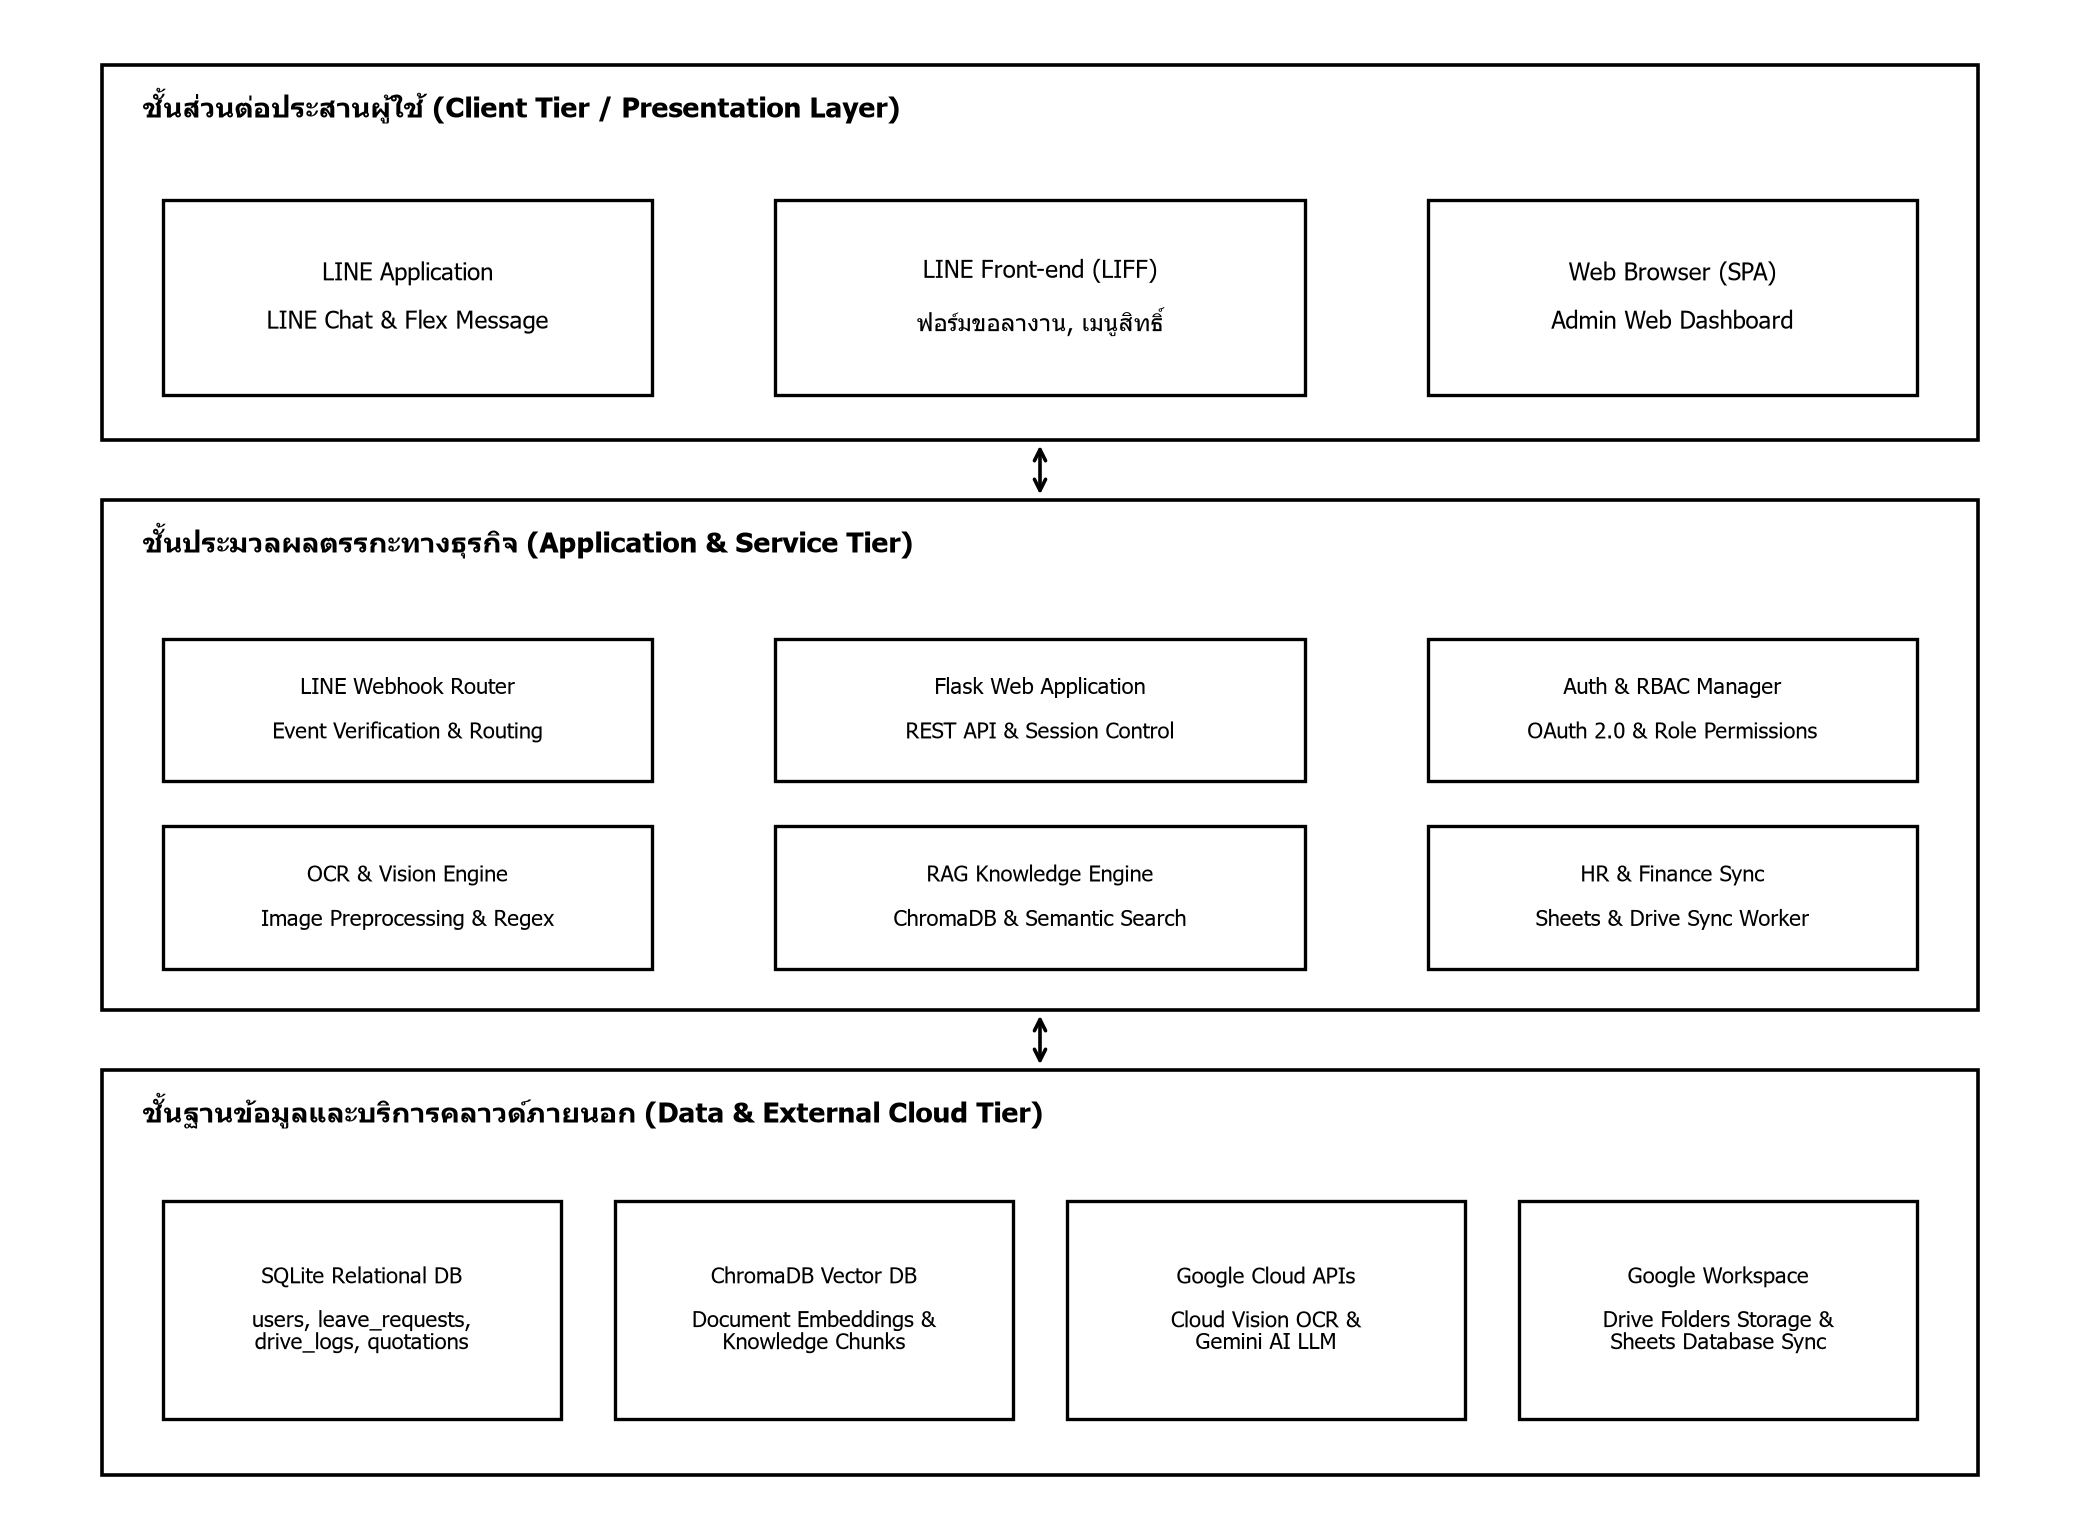
\includegraphics[width=0.95\textwidth]{Image/fig2_1_architecture.png}
\caption{สถาปัตยกรรมระบบปัญญาประดิษฐ์แชทบอทสำหรับองค์กร (System Architecture Diagram)}
\label{fig2:architecture}
\end{figure}

\section{แพลตฟอร์มและการเชื่อมต่อ LINE (Messaging API \& LIFF)}

\subsection{LINE Messaging API}
\hspace*{1.3em}
เป็นชุดเครื่องมือที่ช่วยให้นักพัฒนาสามารถส่งข้อความแบบสองทาง (Two-way communication) ระหว่างผู้ใช้งาน LINE กับเซิร์ฟเวอร์ของระบบ โดยเซิร์ฟเวอร์จะรับ Webhook Event ผ่าน HTTPS POST request พร้อมการตรวจสอบความถูกต้องของลายเซ็นดิจิทัล (X-Line-Signature) ด้วยอัลกอริทึม HMAC-SHA256 เพื่อป้องกันการปลอมแปลงคำขอ

\subsection{LINE Front-end Framework (LIFF)}
\hspace*{1.3em}
เป็นแพลตฟอร์มสำหรับแสดงผลเว็บแอปพลิเคชันภายในแอปพลิเคชัน LINE ช่วยให้ผู้ใช้สามารถเปิดหน้าจอเว็บ เช่น หน้าฟอร์มยื่นคำขอลางาน หรือหน้าระบบรายงาน โดยไม่ต้องออกจากแอป LINE

\subsection{LINE Flex Message}
\hspace*{1.3em}
สถาปัตยกรรมการแสดงผลข้อความในรูปแบบการ์ดที่สามารถจัดวางโครงสร้างคล้ายหน้าเว็บ (CSS Flexible Box) สามารถกำหนดสี ขนาดตัวอักษร การจัดวางปุ่มกด Call-to-Action (เช่น ปุ่ม "อนุมัติ" / "ปฏิเสธ" การลา)

\section{ทฤษฎีการจัดการฐานข้อมูลและสถาปัตยกรรมมัลติเทแนนต์ (Database \& Multi-Tenant)}

\subsection{ทฤษฎีการออกแบบฐานข้อมูลเชิงสัมพันธ์และกระบวนการนอร์มัลไลเซชัน (Database Normalization)}
\hspace*{1.3em}
การออกแบบตารางข้อมูลในระบบ OrgChat AI ผ่านกระบวนการนอร์มัลไลเซชันให้อยู่ในระดับ 3NF (Third Normal Form) เพื่อลดความซ้ำซ้อนของข้อมูล และกำหนดคีย์หลัก (Primary Key) ร่วมกับคีย์นอก (Foreign Key) เพื่อรักษา Referential Integrity

\subsection{คุณสมบัติ ACID ของการทำธุรกรรม (ACID Properties)}
\hspace*{1.3em}
รับประกันคุณสมบัติ Atomicity, Consistency, Isolation และ Durability โดยเฉพาะการตัดโควตาวันลาและการลงบัญชี

\subsection{สถาปัตยกรรมแยกข้อมูลระหว่างองค์กร (Multi-Tenant Data Isolation)}
\hspace*{1.3em}
ใช้โมเดล Shared Database with Tenant-Specific Partitioning โดยทุกตารางข้อมูลหลักจะมีคอลัมน์ \texttt{org\_id} กำกับไว้เพื่อป้องกันการเข้าถึงข้อมูลข้ามองค์กร

\section{ทฤษฎีความปลอดภัยและการควบคุมสิทธิ์การเข้าถึง (Information Security \& RBAC)}

\subsection{การควบคุมการเข้าถึงตามบทบาท (Role-Based Access Control: RBAC)}
\hspace*{1.3em}
ระบบกำหนดสิทธิ์การใช้งานแบ่งตามระดับบทบาทหน้าที่ 5 ระดับ ได้แก่ Super Administrator, Organization Admin, Manager, Employee และ General User ยึดตามมาตรฐาน NIST (2020)

\subsection{ความปลอดภัยของรหัสผ่านและการจัดการเซสชัน}
\hspace*{1.3em}
ใช้ฟังก์ชันแฮชทางเดียว PBKDF2/Bcrypt พร้อม Salt สุ่ม ร่วมกับการจัดการเซสชันที่ปลอดภัย คุกกี้ HttpOnly, Secure และ SameSite

\subsection{การรักษาความสมบูรณ์ของเอกสารและบันทึกตรวจสอบ (File Integrity \& Audit Logging)}
\hspace*{1.3em}
คำนวณค่าแฮช SHA-256 สำหรับไฟล์เอกสารทุกฉบับ พร้อมบันทึกประวัติการกระทำสำคัญลงใน Audit Logs

\section{การเชื่อมต่อบริการคลาวด์ภายนอก (Google Cloud \& Workspace APIs)}

\subsection{Google Drive API}
\hspace*{1.3em}
จัดเก็บไฟล์เอกสารและสลิปแบบแยกโฟลเดอร์ตามปี พ.ศ. และเดือนโดยอัตโนมัติ

\subsection{Google Sheets API}
\hspace*{1.3em}
บันทึกข้อมูลการเงินรายรับ-รายจ่ายเป็นสมุดบัญชีออนไลน์แบบเรียลไทม์

\section{ทฤษฎีการออกแบบส่วนต่อประสานผู้ใช้และการแสดงผลข้อมูลเชิงภาพ (UI/UX \& Data Visualization)}
\hspace*{1.3em}
ยึดหลักการ 10 ประการของ Jakob Nielsen (Usability Heuristics) ร่วมกับการใช้ไลบรารี Chart.js ในการสร้างกราฟแท่ง กราฟวงกลม และกราฟเส้นแสดงสถิติภาพรวมบนแผงควบคุม

\section{ซอฟต์แวร์และเครื่องมือที่ใช้ในการพัฒนา (Development Tools \& Software)}
\hspace*{1.3em}
ในการดำเนินงานจัดทำโครงงานพิเศษนี้ คณะผู้จัดทำได้เลือกใช้เครื่องมือและซอฟต์แวร์มาตรฐานในวิศวกรรมซอฟต์แวร์ ดังนี้:

\noindent\hspace*{1.3em}\textbf{1) Visual Studio Code (VS Code):} โปรแกรมแก้ไขโค้ดหลัก รองรับส่วนขยายสำหรับการเขียนโค้ดภาษา Python, HTML5, CSS และการจัดการสภาพแวดล้อมเสมือน\par\vspace{0.25em}
\noindent\hspace*{1.3em}\textbf{2) Python 3.10+ และ Flask Framework:} ภาษาโปรแกรมและเว็บเฟรมเวิร์กฝั่งเซิร์ฟเวอร์หลัก ใช้ในการจัดการเส้นทาง API, Webhook Handler และการเชื่อมต่อ AI โมเดล\par\vspace{0.25em}
\noindent\hspace*{1.3em}\textbf{3) SQLite และ ChromaDB:} SQLite ใช้สำหรับจัดเก็บข้อมูลเชิงสัมพันธ์ของผู้ใช้งานและองค์กร ขณะที่ ChromaDB เป็นฐานข้อมูลเวกเตอร์ประสิทธิภาพสูงสำหรับระบบ RAG\par\vspace{0.25em}
\noindent\hspace*{1.3em}\textbf{4) Git และ GitHub:} ระบบควบคุมเวอร์ชันซอฟต์แวร์แบบกระจายศูนย์ ใช้ในการบันทึกประวัติการพัฒนาโค้ดและทำงานร่วมกันในทีม\par\vspace{0.25em}
\noindent\hspace*{1.3em}\textbf{5) Figma:} เครื่องมือออกแบบส่วนต่อประสานผู้ใช้ (UI/UX) และจำลองต้นแบบหน้าจอ (Interactive Prototype) ก่อนการพัฒนาจริง\par\vspace{0.25em}
\noindent\hspace*{1.3em}\textbf{6) Google Antigravity:} แพลตฟอร์มพัฒนาระบบตัวแทนปัญญาประดิษฐ์ (Agentic AI) สำหรับช่วยทดสอบและพัฒนาโมดูลการทำงานอัตโนมัติ\par\vspace{0.4em}

\section{งานวิจัยและระบบงานที่เกี่ยวข้อง}

\subsection{การทบทวนวรรณกรรมและงานวิจัยที่เกี่ยวข้อง (Related Literature Review)}
\hspace*{1.3em}
จากการทบทวนวรรณกรรมและงานวิจัยที่เกี่ยวข้องกับการประยุกต์ใช้เทคโนโลยีปัญญาประดิษฐ์และระบบจัดการองค์กร คณะผู้จัดทำได้ศึกษาและนำแนวคิดจากงานวิจัยสำคัญมาประยุกต์ใช้ ดังนี้:

\hspace*{1.3em}
\textbf{1) งานวิจัยด้านระบบการค้นคืนข้อมูลเสริมด้วยปัญญาประดิษฐ์ (RAG):} สมชาย สถิตธรรม และคณะ (2566) ได้ศึกษาวิจัยเรื่อง "การพัฒนาระบบตอบคำถามอัตโนมัติด้วยโมเดลภาษาขนาดใหญ่ร่วมกับเทคนิคการค้นคืนข้อมูลเสริม (RAG)" ในการประชุมวิชาการระดับชาติด้านคอมพิวเตอร์และเทคโนโลยีสารสนเทศ (NCCIT 2023) ผลการวิจัยพบว่า การผสานเทคนิค RAG ร่วมกับ Vector Database ช่วยลดอัตราการสร้างข้อมูลที่ไม่ถูกต้อง (Hallucination) ของโมเดลภาษาขนาดใหญ่ได้อย่างมีประสิทธิภาพ และเพิ่มความแม่นยำในการตอบคำถามเฉพาะทาง คณะผู้จัดทำจึงนำแนวทางนี้มาประยุกต์ใช้สร้างคลังความรู้อัจฉริยะสำหรับข้อมูลสินค้าและระเบียบปฏิบัติงานของ บริษัท ฮาร์ทวอมมิ่ง จำกัด

\hspace*{1.3em}
\textbf{2) งานวิจัยด้านการรู้จำอักขระจากสลิปโอนเงิน (OCR):} กิตติศักดิ์ เจริญชัยภาณุพงศ์ และ ภาณุพงศ์ วงศ์สวัสดิ์ (2565) ได้ศึกษาวิจัยเรื่อง "การรู้จำอักขระจากสลิปโอนเงินผ่านโมบายแบงกิ้งด้วยเทคนิคการประมวลผลภาพดิจิทัล" ในวารสารเทคโนโลยีสารสนเทศและนวัตกรรม ผลการวิจัยระบุว่า การเตรียมภาพล่วงหน้า (Image Preprocessing) ร่วมกับการใช้นิพจน์ปกติ (Regular Expression) ช่วยให้ระบบสามารถสกัดฟิลด์ยอดเงิน วันที่ และเลขอ้างอิงจากสลิปธนาคารได้อย่างแม่นยำสูง คณะผู้จัดทำจึงได้นำเทคนิคการปรับภาพและการสกัดฟิลด์ข้อมูลด้วย Regex มาพัฒนาต่อยอดในโมดูลอ่านสลิปและใบเสร็จอัตโนมัติ

\hspace*{1.3em}
\textbf{3) งานวิจัยด้านระบบบริการผ่าน LINE Platform:} การศึกษาการพัฒนาระบบบริการผ่าน LINE Messaging API และ LINE Flex Message พบว่า การผสานระบบสารสนเทศเข้ากับแอปพลิเคชันสนทนาช่วยลดแรงต้านของผู้ใช้งาน (Frictionless Experience) เนื่องจากพนักงานมีความคุ้นเคยกับแอปพลิเคชัน LINE อยู่แล้ว จึงสามารถเรียนรู้และใช้งานระบบใหม่ได้อย่างรวดเร็ว

\hspace*{1.3em}
\textbf{4) มาตรฐานความมั่นคงปลอดภัยและการควบคุมสิทธิ์ตามบทบาท (RBAC):} ยึดตามมาตรฐาน Role-Based Access Control ของสถาบัน NIST (2020) ในการกำหนดสิทธิ์ผู้ใช้งานเป็นระดับชั้น (Super Admin, Org Admin, Manager, Employee, General User) ร่วมกับกลไกแยกข้อมูล Multi-Tenant เพื่อรับประกันความปลอดภัยของข้อมูลองค์กรตามพระราชบัญญัติคุ้มครองข้อมูลส่วนบุคคล (PDPA)

\subsection{ตารางเปรียบเทียบคุณสมบัติระบบกับระบบงานในท้องตลาด}
\hspace*{1.3em}
จากการสำรวจงานวิจัยและระบบงานที่เกี่ยวข้อง คณะผู้จัดทำได้นำคุณสมบัติของระบบปัญญาประดิษฐ์แชทบอทสำหรับองค์กรที่พัฒนาขึ้น (OrgChat AI) มาวิเคราะห์เปรียบเทียบกับซอฟต์แวร์สื่อสารและบริหารจัดการองค์กรชั้นนำในท้องตลาด ดังแสดงในตารางที่ 2-1:

\begin{table}[htbp]
\centering
\caption{ตารางเปรียบเทียบคุณสมบัติระบบที่พัฒนากับแอปพลิเคชันอื่นในท้องตลาด}
\label{tab2:comparison}
\begin{tabularx}{\textwidth}{| L | >{\centering\arraybackslash}p{1.7cm} | >{\centering\arraybackslash}p{1.4cm} | >{\centering\arraybackslash}p{1.5cm} | >{\centering\arraybackslash}p{1.7cm} | >{\centering\arraybackslash}p{1.6cm} |}
\hline
\textbf{คุณสมบัติการทำงาน} & \textbf{ระบบที่พัฒนา\ (OrgChat)} & \textbf{Slack} & \textbf{MS Teams} & \textbf{ChatGPT\ Ent.} & \textbf{LINE\ WORKS} \\ \hline
1. ใช้งานผ่านแอปพลิเคชัน LINE ปกติ & \cmark & \xmark & \xmark & \xmark & \xmark \\ \hline
2. เข้าสู่ระบบด้วย LINE Login OAuth & \cmark & \xmark & \xmark & \xmark & \xmark \\ \hline
3. แชทบอท AI ภาษาธรรมชาติ (LLM) & \cmark & \cmark & \cmark & \cmark & \xmark \\ \hline
4. คลังความรู้เอกสารองค์กร (RAG) & \cmark & \xmark & \xmark & \cmark & \xmark \\ \hline
5. รองรับไฟล์หลายรูปแบบ (PDF, DOCX, XLS) & \cmark & \cmark & \cmark & \cmark & \cmark \\ \hline
6. OCR อ่านสลิปโอนเงินและใบเสร็จ & \cmark & \xmark & \xmark & \xmark & \xmark \\ \hline
7. บันทึกบัญชีอัตโนมัติลง Google Sheets & \cmark & \xmark & \xmark & \xmark & \xmark \\ \hline
8. ระบบกระทบยอดสลิปและใบกำกับภาษี & \cmark & \xmark & \xmark & \xmark & \xmark \\ \hline
9. ระบบยื่นและอนุมัติใบลาผ่านแชท & \cmark & \xmark & \xmark & \xmark & \cmark \\ \hline
10. ควบคุมสิทธิ์ตามบทบาท (RBAC) & \cmark & \cmark & \cmark & \cmark & \cmark \\ \hline
11. แจ้งเตือนอัตโนมัติผ่าน LINE Flex & \cmark & \xmark & \xmark & \xmark & \xmark \\ \hline
12. จัดระเบียบไฟล์บน Google Drive อัตโนมัติ & \cmark & \xmark & \xmark & \xmark & \xmark \\ \hline
13. แผงควบคุมและกราฟสรุปผล (Dashboard) & \cmark & \xmark & \cmark & \xmark & \xmark \\ \hline
14. ระบบจัดการใบเสนอราคาและ CRM ในตัว & \cmark & \xmark & \xmark & \xmark & \xmark \\ \hline
15. เหมาะกับ SMEs ไทย / ค่าใช้จ่ายประหยัด & \cmark & \xmark & \xmark & \xmark & \xmark \\ \hline
\end{tabularx}
\end{table}

\subsection{ตารางการเปรียบเทียบงานวิจัยที่เกี่ยวข้องกับโครงงาน}
\hspace*{1.3em}
จากการทบทวนวรรณกรรม คณะผู้จัดทำได้ทำการวิเคราะห์และสังเคราะห์เปรียบเทียบงานวิจัยที่เกี่ยวข้องกับการพัฒนาระบบแชทบอท ปัญญาประดิษฐ์คลังความรู้ และระบบสารสนเทศ เพื่อนำข้อดีและแนวทางมาประยุกต์ใช้ในโครงงาน ดังแสดงในตารางที่ 2-2:

\begin{table}[htbp]
\centering
\caption{ตารางการเปรียบเทียบงานวิจัยที่เกี่ยวข้องกับโครงงาน}
\label{tab2:research_comp}
\begin{tabularx}{\textwidth}{| L | L | L | L |}
\hline
\textbf{ผู้วิจัยและปีที่พิมพ์} & \textbf{ชื่องานวิจัย / หัวข้อ} & \textbf{เทคโนโลยีที่ใช้} & \textbf{การนำมาประยุกต์ใช้ในโครงงาน} \\ \hline
สมชาย สถิตธรรม และคณะ (2566) & การพัฒนาระบบตอบคำถามอัตโนมัติด้วยโมเดลภาษาขนาดใหญ่ร่วมกับเทคนิค RAG & LangChain, ChromaDB, OpenAI GPT & นำเทคนิค RAG และ Vector Search มาประยุกต์ใช้กับ Google Gemini และ FastEmbed เพื่อตอบคำถามจากคู่มือสินค้าขององค์กร \\ \hline
กิตติศักดิ์ เจริญชัยภาณุพงศ์ และ ภาณุพงศ์ วงศ์สวัสดิ์ (2565) & การรู้จำอักขระจากสลิปโอนเงินผ่านโมบายแบงกิ้งด้วยเทคนิคการประมวลผลภาพดิจิทัล & Tesseract OCR, OpenCV, Regular Expression & นำหลักการเตรียมภาพดิจิทัล (Binarization, Deskew) และ Regex ไปใช้อ่านสลิปและใบเสร็จในแผนงานระบบการเงิน \\ \hline
Lewis et al. (2020) & Retrieval-Augmented Generation for Knowledge-Intensive NLP Tasks & Dense Passage Retrieval (DPR), BART & นำแนวคิดการเชื่อมโยงคลังข้อมูลเวกเตอร์เข้ากับโมเดลภาษามาใช้เพื่อลดปัญหา Hallucination ของ AI \\ \hline
นริศรา บุญช่วย และคณะ (2566) & การพัฒนาระบบบริการลูกค้าผ่าน LINE Official Account ร่วมกับเว็บแอปพลิเคชัน & LINE Messaging API, Webhook, Python & ประยุกต์ใช้สถาปัตยกรรม Webhook แบบสองทาง และการส่ง Flex Message เพื่อให้ผู้ใช้สื่อสารได้สะดวกรวดเร็ว \\ \hline
\end{tabularx}
\end{table}


    %*************************************
% บทที่ 3
%*************************************
\chapterTitle{3}{วิธีการดำเนินงานและการออกแบบระบบ}
\vspace{0.2in}
\hspace*{1.3em}
ในบทนี้จะกล่าวถึงระเบียบวิธีการดำเนินงาน ขั้นตอนการดำเนินงานตามวงจรพัฒนาซอฟต์แวร์ การวิเคราะห์ความต้องการของระบบ แผนภาพสถาปัตยกรรมระบบ แผนภาพกระแสข้อมูล (Data Flow Diagram: DFD) ข้อกำหนดลักษณะการประมวลผล (Process Specification: PSPEC) พจนานุกรมข้อมูล (Data Flow Dictionary) การออกแบบข้อมูล (Data Element Description) ผังงานกระบวนการประมวลผล (Process Flowcharts) แบบจำลองความสัมพันธ์ของข้อมูล (ER Diagram) โครงสร้างตารางฐานข้อมูล (Table Layout) ตลอดจนการออกแบบส่วนต่อประสานผู้ใช้ (User Interface Design) สำหรับระบบปัญญาประดิษฐ์แชทบอทสำหรับองค์กร กรณีศึกษา บริษัท ฮาร์ทวอมมิ่ง จำกัด ตามขอบเขตการดำเนินงานในภาคการศึกษาที่ 1/2569

\section{ขั้นตอนและแผนการดำเนินงาน}
\hspace*{1.3em}
การจัดทำโครงงานพิเศษนี้ประยุกต์ใช้วงจรการพัฒนาระบบแบบอไจลส์ (Agile Software Development) ร่วมกับกรอบการทำงานสกรัม (Scrum Framework) ซึ่งเน้นการพัฒนาแบบวนซ้ำและเพิ่มพูนทีละส่วน (Iterative and Incremental Development) โดยแบ่งการดำเนินงานออกเป็น 2 ภาคการศึกษา แผนการดำเนินงานแสดงดังตารางที่ 3-1 และตารางที่ 3-2:

\begin{table}[htbp]
\centering
\caption{แผนการดำเนินงาน ภาคการศึกษาที่ 1/2569}
\label{tab3:plan_term1}
\begin{tabularx}{\textwidth}{| L | c | c | c | c |}
\hline
\textbf{กิจกรรมการดำเนินงาน} & \textbf{เดือนที่ 1} & \textbf{เดือนที่ 2} & \textbf{เดือนที่ 3} & \textbf{เดือนที่ 4} \\ \hline
1. ศึกษาความเป็นมาของ บริษัท ฮาร์ทวอมมิ่ง จำกัด และรวบรวมความต้องการ & \cmark & & & \\ \hline
2. ศึกษาทฤษฎี RAG, Vector Database, LINE API และ Google Cloud & \cmark & \cmark & & \\ \hline
3. วิเคราะห์และออกแบบระบบ (DFD, PSPEC, ERD, Data Dictionary) & & \cmark & & \\ \hline
4. พัฒนาระบบยืนยันตัวตน สมาชิก และ Google OAuth 2.0 & & \cmark & \cmark & \\ \hline
5. พัฒนาระบบคลังความรู้ RAG, Text Chunking และ ChromaDB & & & \cmark & \\ \hline
6. เชื่อมต่อ LINE Messaging API, Webhook และสร้าง LINE Flex Message & & & \cmark & \cmark \\ \hline
7. เชื่อมต่อระบบจัดระเบียบไฟล์บน Google Drive API & & & & \cmark \\ \hline
8. ทดสอบระบบเบื้องต้น (Black-Box Testing) และจัดทำรายงานโปรเจค 100 & & & & \cmark \\ \hline
\end{tabularx}
\end{table}

\begin{table}[htbp]
\centering
\caption{แผนการดำเนินงาน ภาคการศึกษาที่ 2/2569}
\label{tab3:plan_term2}
\begin{tabularx}{\textwidth}{| L | c | c | c | c |}
\hline
\textbf{กิจกรรมการดำเนินงาน} & \textbf{เดือนที่ 1} & \textbf{เดือนที่ 2} & \textbf{เดือนที่ 3} & \textbf{เดือนที่ 4} \\ \hline
1. พัฒนาระบบ OCR สกัดข้อมูลสลิปโอนเงินและใบเสร็จรับเงิน & \cmark & \cmark & & \\ \hline
2. พัฒนาระบบลงบัญชีอัตโนมัติลง Google Sheets และระบบกระทบยอด & & \cmark & & \\ \hline
3. พัฒนาระบบบริหารงานบุคคล (การขอลางาน, การอนุมัติผ่าน LINE Flex) & & \cmark & \cmark & \\ \hline
4. พัฒนาแผงควบคุมผู้บริหาร (Admin Dashboard) และระบบวิเคราะห์ข้อมูล & & & \cmark & \\ \hline
5. ทดสอบระบบเต็มรูปแบบ (System Integration \& Performance Testing) & & & \cmark & \cmark \\ \hline
6. นำระบบไปทดลองใช้งานจริงกับพนักงาน บริษัท ฮาร์ทวอมมิ่ง จำกัด & & & & \cmark \\ \hline
7. ประเมินความพึงพอใจของผู้ใช้งาน และจัดทำปริญญานิพนธ์ฉบับสมบูรณ์ & & & & \cmark \\ \hline
\end{tabularx}
\end{table}

\begin{table}[htbp]
\centering
\caption{เครื่องมือและเทคโนโลยีที่ใช้ในการพัฒนาระบบ}
\label{tab3:tools}
\begin{tabularx}{\textwidth}{| c | L | L |}
\hline
\textbf{ประเภท} & \textbf{เครื่องมือ / เทคโนโลยี} & \textbf{วัตถุประสงค์การใช้งาน} \\ \hline
ฮาร์ดแวร์ & คอมพิวเตอร์ส่วนบุคคล (RAM 16GB, CPU Core i7) & พัฒนา ประมวลผล และทดสอบระบบ \\ \hline
ฮาร์ดแวร์ & สมาร์ตโฟนระบบปฏิบัติการ iOS และ Android & ทดสอบการใช้งานแอปพลิเคชัน LINE OA \\ \hline
ภาษาและเฟรมเวิร์ก & Python 3.10+, Flask Web Framework & พัฒนาเซิร์ฟเวอร์ Backend และ Webhook Handler \\ \hline
ส่วนต่อประสานผู้ใช้ & HTML5, CSS3, JavaScript, Bootstrap & พัฒนาหน้าจอเว็บแอปพลิเคชันฝั่ง Frontend \\ \hline
ฐานข้อมูลเชิงสัมพันธ์ & SQLite Database & จัดเก็บข้อมูลบัญชีผู้ใช้ องค์กร และบันทึกประวัติ \\ \hline
ฐานข้อมูลเวกเตอร์ & ChromaDB ร่วมกับ FastEmbed & จัดเก็บและสืบค้นเวกเตอร์เอ็มเบดดิงในระบบ RAG \\ \hline
ปัญญาประดิษฐ์ & Google Gemini 1.5 Flash API & โมเดลภาษาขนาดใหญ่สังเคราะห์คำตอบภาษาธรรมชาติ \\ \hline
บริการภายนอก & LINE Messaging API & รับ-ส่งข้อความและเชื่อมต่อแชทบอทบน LINE OA \\ \hline
บริการภายนอก & Google Drive API & จัดเก็บไฟล์เอกสารและแยกโฟลเดอร์ตามวันที่ \\ \hline
เครื่องมือควบคุม & Git, GitHub, Visual Studio Code & จัดการเวอร์ชันซอร์สโค้ดและสภาพแวดล้อมพัฒนา \\ \hline
\end{tabularx}
\end{table}

\section{การวิเคราะห์ความต้องการของระบบ}

\subsection{ความต้องการเชิงหน้าที่ (Functional Requirements)}
\hspace*{1.3em}
ความต้องการเชิงหน้าที่ของระบบในภาคการศึกษาที่ 1/2569 ประกอบด้วย:
\begin{mycustomitem}
\item FR-1: ระบบยืนยันตัวตนและจัดการบัญชีผู้ใช้ รองรับการสมัครสมาชิก เข้าสู่ระบบด้วย Email/Password, Google OAuth 2.0 และระบบผูกบัญชี LINE พร้อมการจัดการโปรไฟล์
\end{mycustomitem}
\begin{mycustomitem}
\item FR-2: ระบบคลังความรู้อัจฉริยะ (RAG System) รองรับการอัปโหลดไฟล์เอกสาร (PDF, TXT, สเปรดชีต) สกัดข้อความ แบ่งท่อนข้อความ (Chunking) และแปลงเป็นเวกเตอร์เอ็มเบดดิง
\end{mycustomitem}
\begin{mycustomitem}
\item FR-3: ระบบค้นคืนและตอบคำถามภาษาธรรมชาติ รองรับการค้นคืนข้อมูลด้วยความคล้ายคลึงแบบโคไซน์ (Cosine Similarity) ใน ChromaDB และสังเคราะห์คำตอบด้วย Google Gemini
\end{mycustomitem}
\begin{mycustomitem}
\item FR-4: ระบบแชทบอท LINE OA เชื่อมต่อผ่าน LINE Messaging API รับส่งข้อความภาษาธรรมชาติและตอบกลับด้วยการ์ด LINE Flex Message ที่มีปุ่มกดโต้ตอบ
\end{mycustomitem}
\begin{mycustomitem}
\item FR-5: ระบบจัดการไฟล์และคลาวด์ รองรับการอัปโหลดและจัดระเบียบไฟล์เอกสารขึ้นสู่ Google Drive แยกโฟลเดอร์ตามวันเวลาอัตโนมัติ
\end{mycustomitem}

\subsection{ความต้องการที่ไม่ใช่เชิงหน้าที่ (Non-Functional Requirements)}
\begin{mycustomitem}
\item NFR-1 ด้านประสิทธิภาพ (Performance): ระบบแชทบอท RAG สามารถค้นคืนข้อมูลและสร้างคำตอบส่งกลับทาง LINE ภายในระยะเวลาไม่เกิน 3-5 วินาที
\end{mycustomitem}
\begin{mycustomitem}
\item NFR-2 ด้านความมั่นคงปลอดภัย (Security): ตรวจสอบความถูกต้องของคำขอผ่านลายเซ็นดิจิทัล X-Line-Signature ด้วย HMAC-SHA256 และเข้ารหัสรหัสผ่านด้วยอัลกอริทึม BCrypt
\end{mycustomitem}
\begin{mycustomitem}
\item NFR-3 ด้านการแยกข้อมูลระหว่างองค์กร (Multi-Tenant Isolation): ออกแบบฐานข้อมูลให้แบ่งแยกข้อมูลระหว่างแต่ละองค์กรด้วย Organization ID
\end{mycustomitem}
\begin{mycustomitem}
\item NFR-4 ด้านความง่ายในการใช้งาน (Usability): ผู้ใช้งานสามารถสอบถามข้อมูลผ่านแอปพลิเคชัน LINE ที่คุ้นเคยได้ทันทีโดยไม่ต้องเรียนรู้โปรแกรมใหม่
\end{mycustomitem}
\begin{mycustomitem}
\item NFR-5 ด้านความพร้อมใช้งาน (Availability): ระบบเซิร์ฟเวอร์สามารถให้บริการต่อเนื่องตลอด 24 ชั่วโมง มีความพร้อมใช้งานไม่น้อยกว่าร้อยละ 99.0
\end{mycustomitem}

\section{การออกแบบสถาปัตยกรรมของระบบ (System Architecture)}
\hspace*{1.3em}
สถาปัตยกรรมของระบบปัญญาประดิษฐ์แชทบอทสำหรับองค์กร ถูกออกแบบตามรูปแบบ Client-Server และ Event-Driven Architecture โดยแบ่งเป็น 3 ส่วนหลัก ได้แก่ 1) ส่วนต่อประสานผู้ใช้ (LINE OA และ Web Frontend), 2) ส่วนประมวลผลเซิร์ฟเวอร์ (Flask Backend, Webhook Handler, RAG Pipeline) และ 3) ส่วนจัดเก็บข้อมูลและบริการภายนอก (SQLite, ChromaDB, Google Gemini, Google Drive) ดังแสดงในภาพที่ 3-1:

\begin{figure}[htbp]
\centering
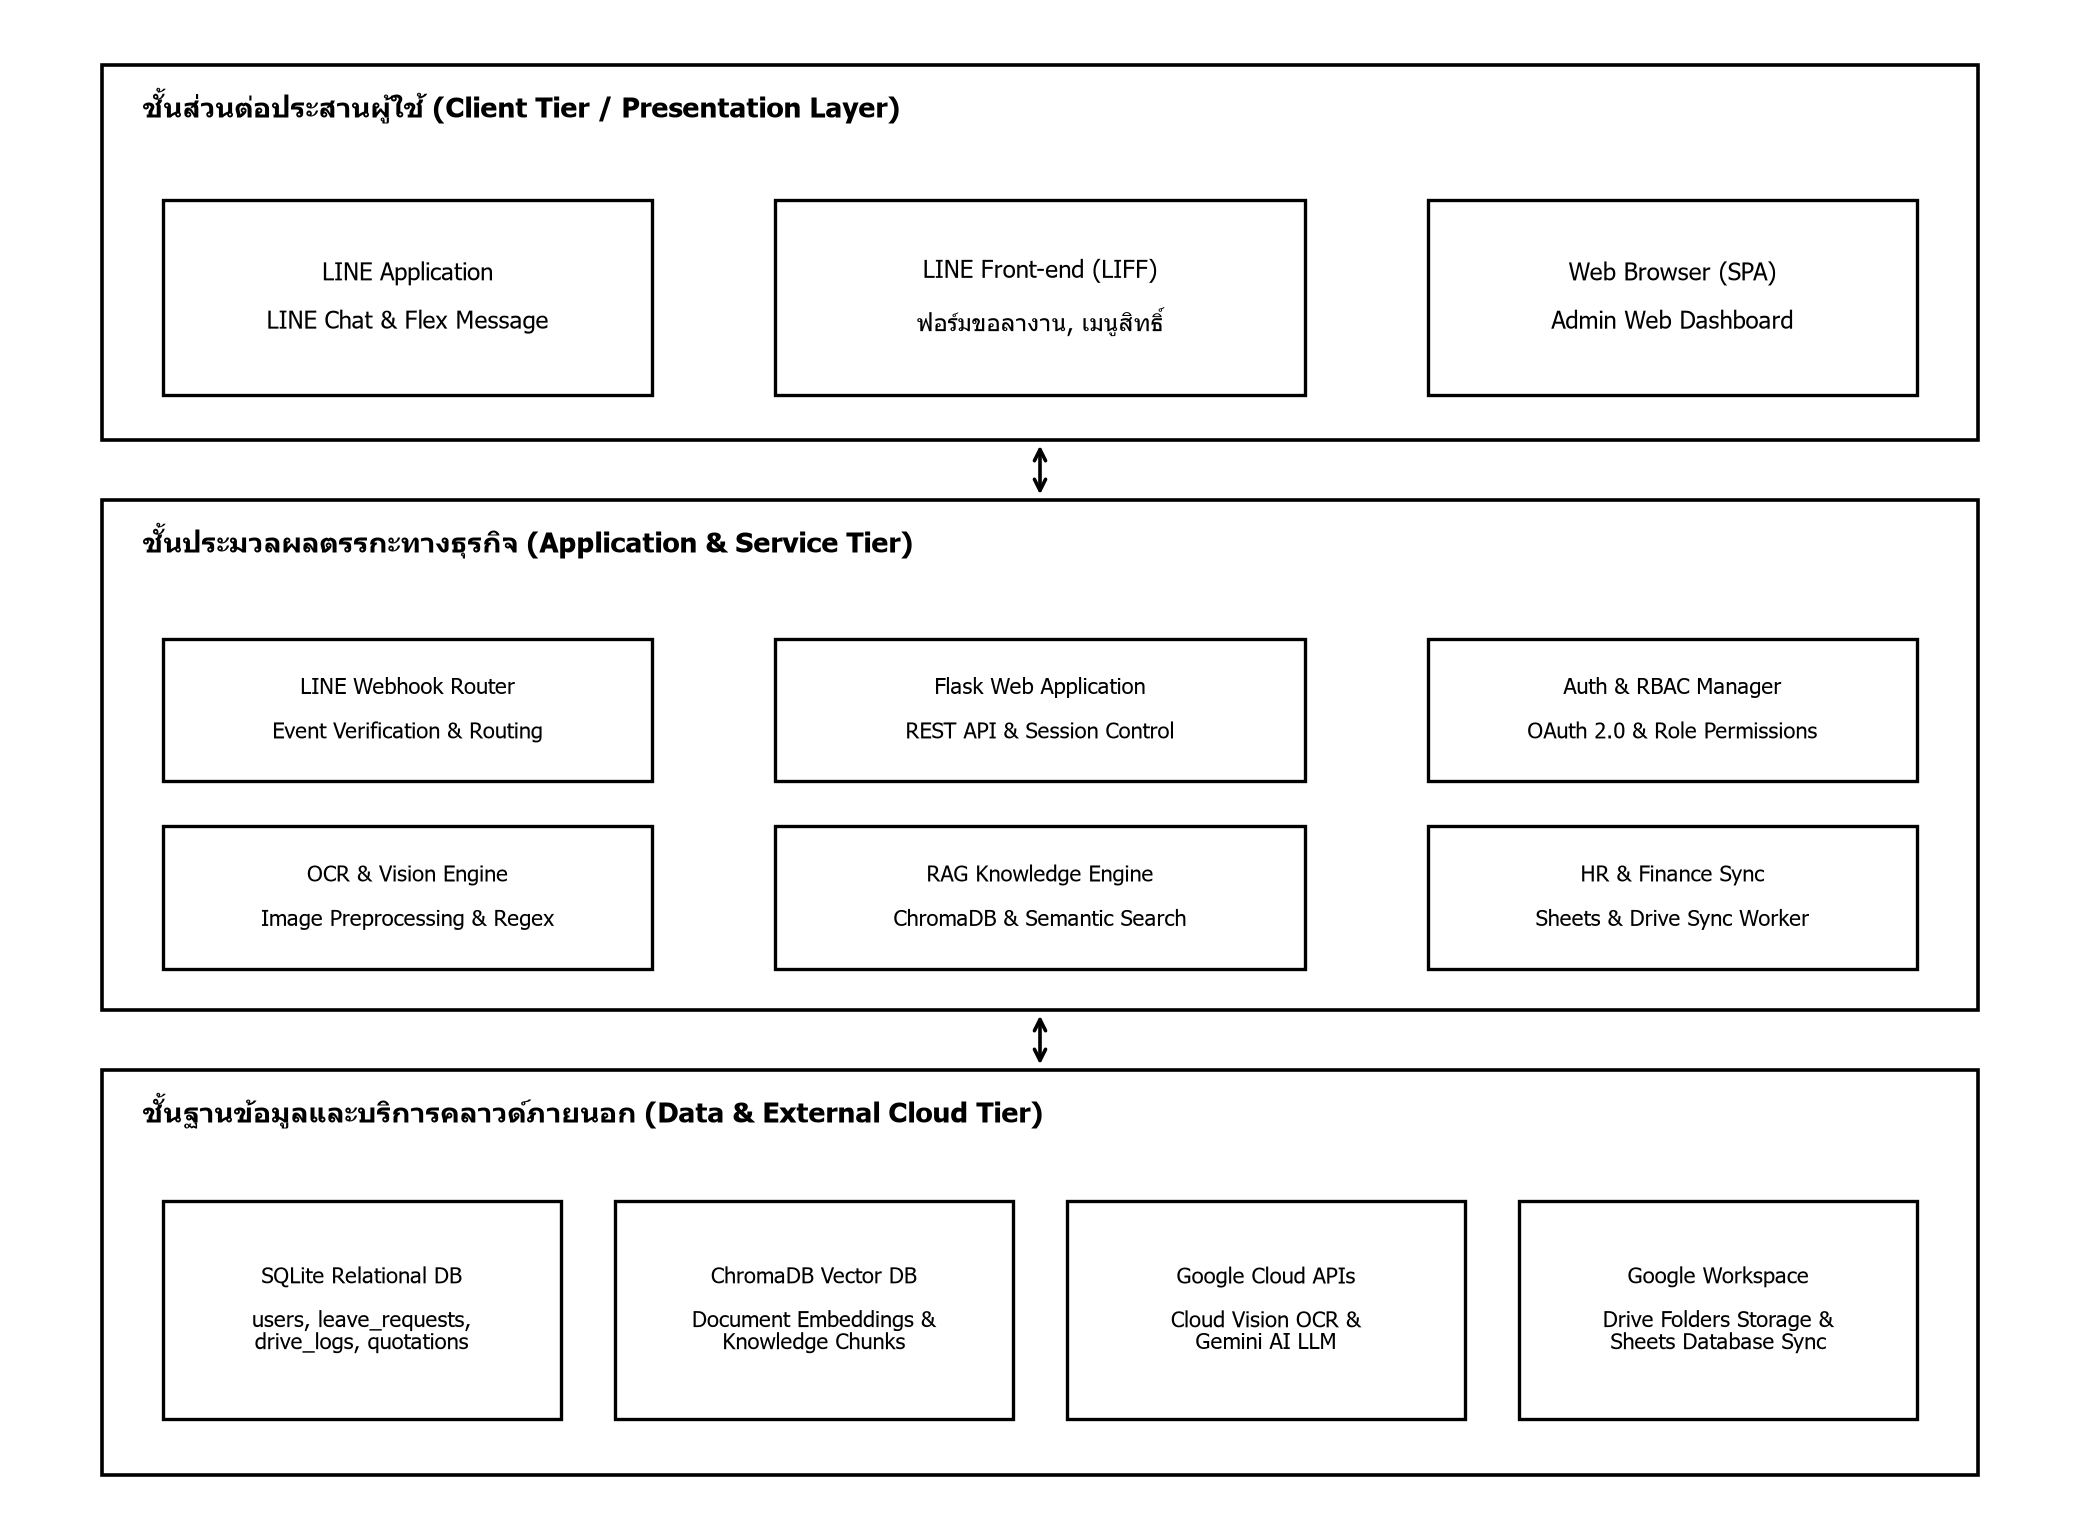
\includegraphics[width=0.95\textwidth]{Image/fig2_1_architecture.png}
\caption{สถาปัตยกรรมของระบบปัญญาประดิษฐ์แชทบอทสำหรับองค์กร (System Architecture Diagram)}
\label{fig3:arch}
\end{figure}

\section{แผนภาพกระแสข้อมูล (Data Flow Diagram: DFD)}
\hspace*{1.3em}
แผนภาพกระแสข้อมูลแสดงการไหลของข้อมูลระหว่างเอนทิตีภายนอก (External Entities) กระบวนการประมวลผล (Processes) และแหล่งจัดเก็บข้อมูล (Data Stores) โดยเริ่มต้นจากแผนภาพบริบท (Context Diagram) และจำแนกออกเป็น DFD ระดับต่าง ๆ

\subsection{แผนภาพบริบท (Context Diagram)}
\hspace*{1.3em}
แผนภาพบริบทแสดงภาพรวมความสัมพันธ์ระหว่างระบบ OrgChat AI กับเอนทิตีภายนอก (External Entities) ทั้งหมด 5 กลุ่ม ได้แก่ 1) พนักงาน (Employee), 2) หัวหน้างาน (Manager), 3) ผู้ดูแลระบบ (Admin), 4) แพลตฟอร์ม LINE (LINE Platform) และ 5) บริการกูเกิลคลาวด์ (Google Cloud APIs: Gemini, Drive) ดังแสดงในภาพที่ 3-2:

\begin{figure}[htbp]
\centering
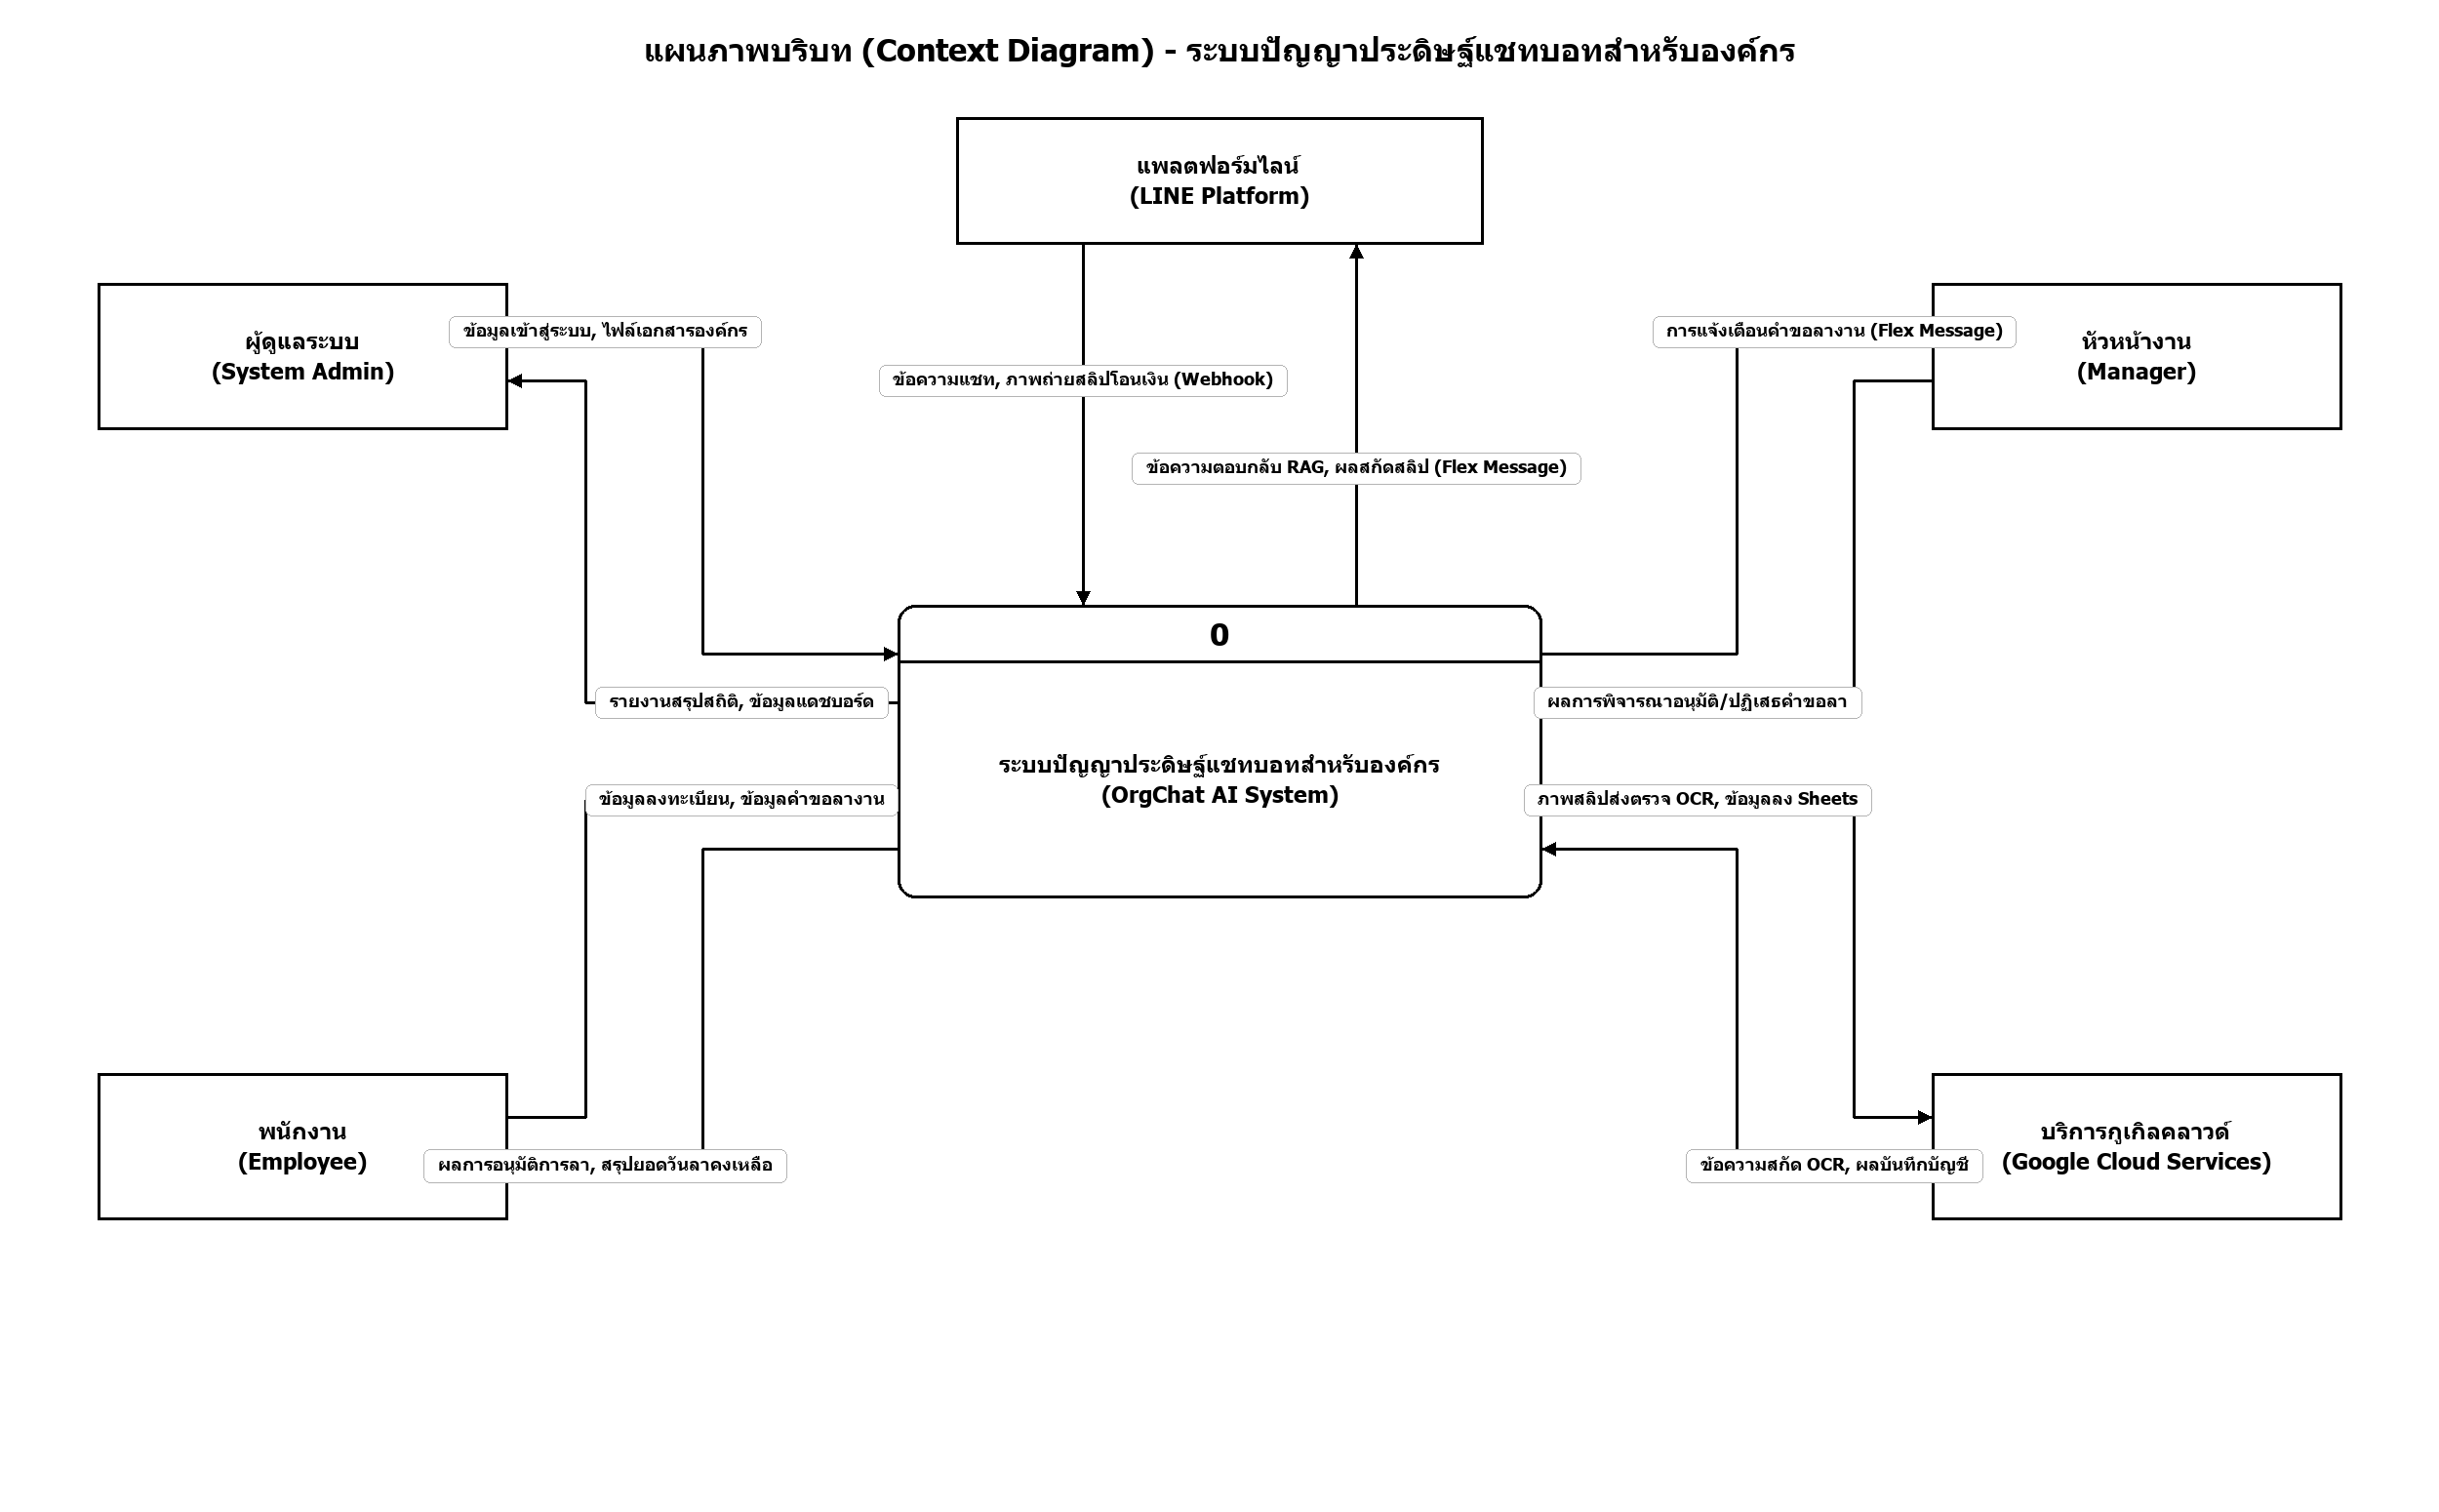
\includegraphics[width=0.95\textwidth]{Image/fig3_1_context.png}
\caption{Context Diagram ของระบบปัญญาประดิษฐ์แชทบอทสำหรับองค์กร}
\label{fig3:context}
\end{figure}

\subsection{แผนภาพกระแสข้อมูลระดับ 0 (DFD Level 0)}
\hspace*{1.3em}
แผนภาพกระแสข้อมูลระดับ 0 (DFD Level 0) แสดงภาพรวมกระบวนการทำงานหลัก 5 กระบวนการที่เชื่อมโยงกับแหล่งจัดเก็บข้อมูล (Data Store D1 - D6) และเอนทิตีภายนอกทั้งหมดของระบบปัญญาประดิษฐ์แชทบอทสำหรับองค์กร ดังแสดงในภาพที่ 3-3:

\begin{figure}[htbp]
\centering
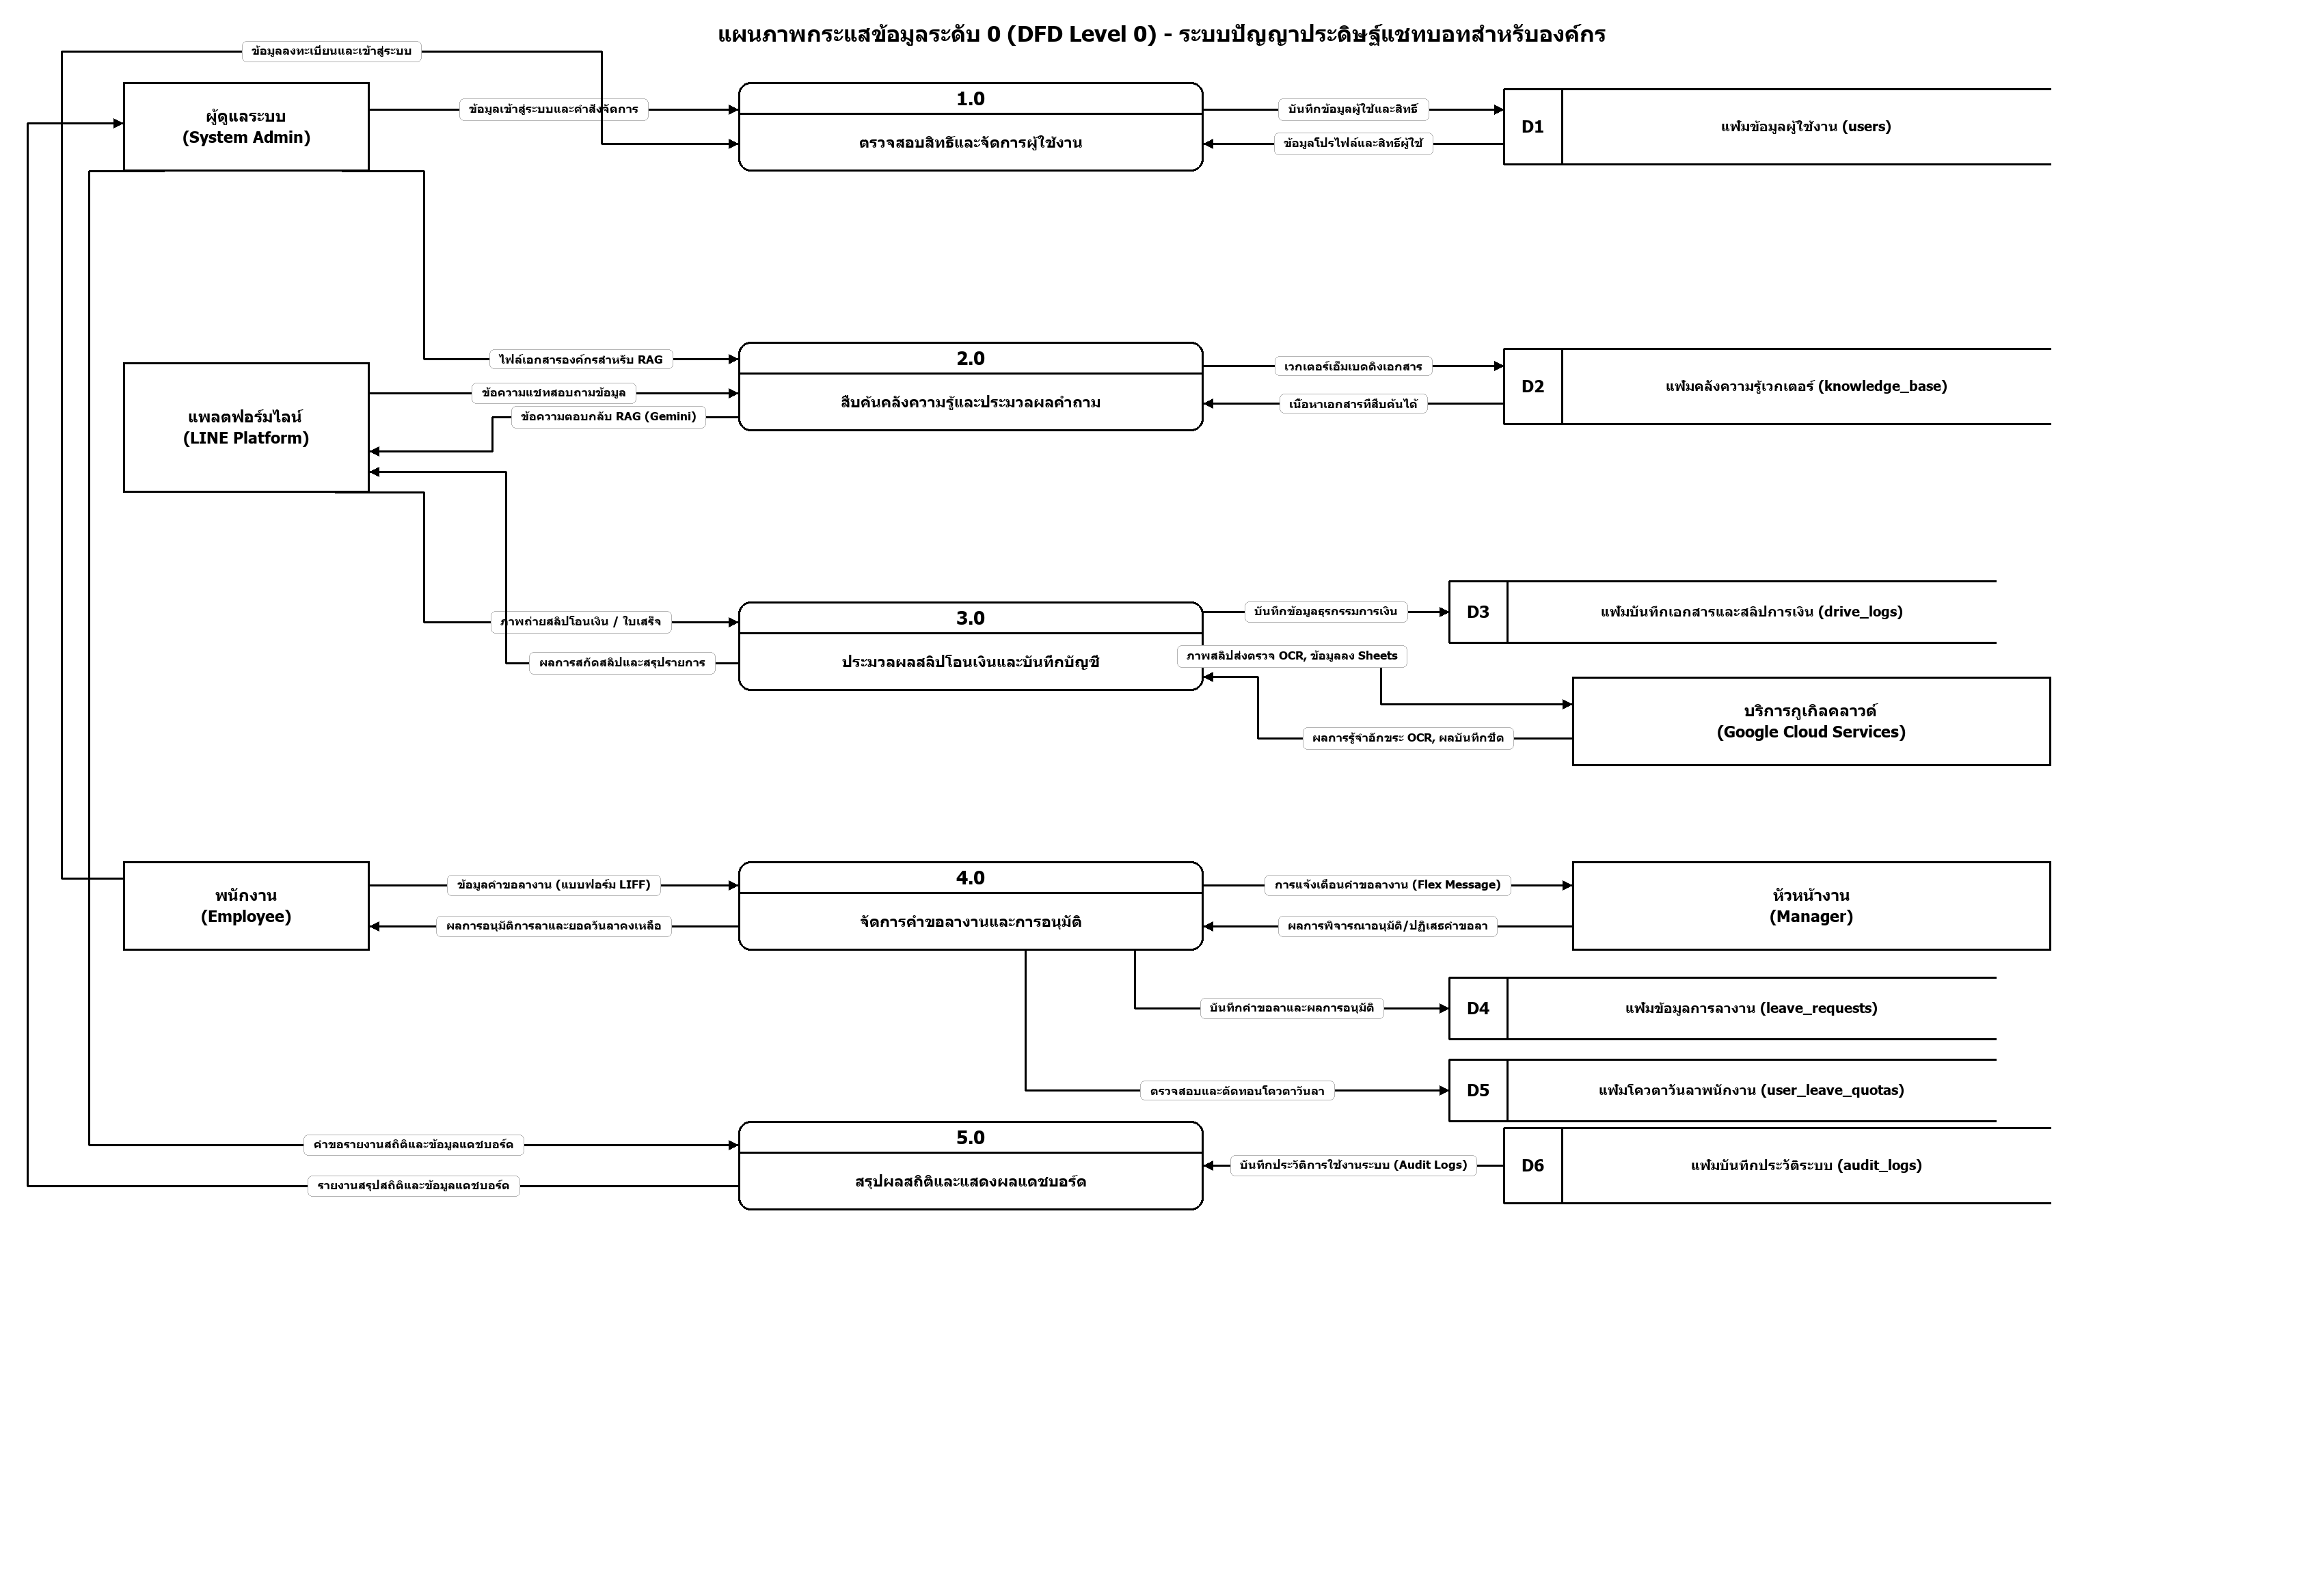
\includegraphics[width=0.95\textwidth]{Image/fig3_2_dfd.png}
\caption{Data Flow Diagram Level 0 ของระบบปัญญาประดิษฐ์แชทบอทสำหรับองค์กร}
\label{fig3:dfd0}
\end{figure}

\hspace*{1.3em}
กระบวนการทำงานหลัก 5 กระบวนการ ประกอบด้วย:
\begin{enumerate}[leftmargin=3.5em]
\item[1.0] ตรวจสอบสิทธิ์และจัดการผู้ใช้งาน (Authenticate \& Manage Users) ทำหน้าที่ตรวจสอบความถูกต้องของการเข้าสู่ระบบ ควบคุมสิทธิ์การใช้งาน (RBAC) และจัดการโปรไฟล์บัญชีผู้ใช้
\item[2.0] สืบค้นคลังความรู้และประมวลผลคำถาม (Retrieve Knowledge \& Process Queries) ทำหน้าที่ตรวจสอบนำเข้าเอกสาร สกัดข้อความ แปลงเป็นเวกเตอร์เอ็มเบดดิง และค้นคืนคำตอบด้วยเทคโนโลยี RAG
\item[3.0] ประมวลผลสลิปโอนเงินและบันทึกบัญชี (Process Payment Slip OCR \& Accounting) ทำหน้าที่รับภาพถ่ายสลิปเงินโอนผ่าน Webhook สกัดข้อมูลด้วย OCR และลงรายการบัญชีบน Google Sheets
\item[4.0] จัดการคำขอลางานและการอนุมัติ (Manage Leave Requests \& Approvals) ทำหน้าที่รับคำขอลางานจากแบบฟอร์ม LIFF แจ้งเตือนหัวหน้างานผ่าน LINE Flex Message และบันทึกผลการอนุมัติ
\item[5.0] สรุปผลสถิติและแสดงผลแดชบอร์ด (Summarize Statistics \& Display Dashboard) ทำหน้าที่รวบรวมประวัติการใช้งานและบันทึกระบบ (Audit Logs) เพื่อประมวลผลแสดงข้อมูลสถิติเชิงภาพบนเว็บแดชบอร์ด
\end{enumerate}

\noindent\textbf{หมายเหตุเชิงสถาปัตยกรรมระบบ (Architectural Scope Note):} แผนภาพบริบท (ภาพที่ 3-2) และแผนภาพกระแสข้อมูลระดับ 0 (ภาพที่ 3-3) แสดงภาพรวมเชิงแนวคิด (Target Architecture) ของระบบ OrgChat AI ทั้งระบบ โดยในภาคการศึกษาที่ 1/2569 (โครงงานพิเศษ 100) คณะผู้จัดทำได้ดำเนินการพัฒนา ทดสอบ และประเมินผลสำเร็จในส่วนกระบวนการหลัก ได้แก่ กระบวนการ 1.0 (ระบบยืนยันตัวตน) และกระบวนการ 2.0 (ระบบคลังความรู้ RAG) ร่วมกับส่วนเชื่อมต่อ LINE Messaging API และ Google Drive เสร็จสมบูรณ์ สำหรับกระบวนการ 3.0 (ประมวลผลสลิป OCR) และกระบวนการ 4.0 (ระบบลางาน) ได้รับการออกแบบเชิงโครงสร้างและจัดทำเป็นระบบต้นแบบการทำงาน (Working Prototype) เพื่อเตรียมต่อยอดและประเมินผลเชิงลึกในโครงงานพิเศษ 200 ต่อไป

\subsection{แผนภาพกระแสข้อมูลระดับ 1 (DFD Level 1) ของระบบคลังความรู้ RAG}
\hspace*{1.3em}
เพื่อแสดงรายละเอียดเชิงลึกของกระบวนการทำงานหลักที่มีความซับซ้อนตามระเบียบวิธีวิเคราะห์และออกแบบระบบ (SA\&D) แผนภาพกระแสข้อมูลระดับ 1 (DFD Level 1) ของกระบวนการ 2.0 (สืบค้นคลังความรู้และประมวลผลคำถาม) ได้แจกแจงกระบวนการย่อยออกเป็น 6 กระบวนการ (กระบวนการ 2.1 ถึง 2.6) ที่เชื่อมโยงกับแหล่งจัดเก็บข้อมูล D2, D3, D4 และโมเดลปัญญาประดิษฐ์ Google Gemini API ดังแสดงในภาพที่ 3-4:

\begin{figure}[htbp]
\centering
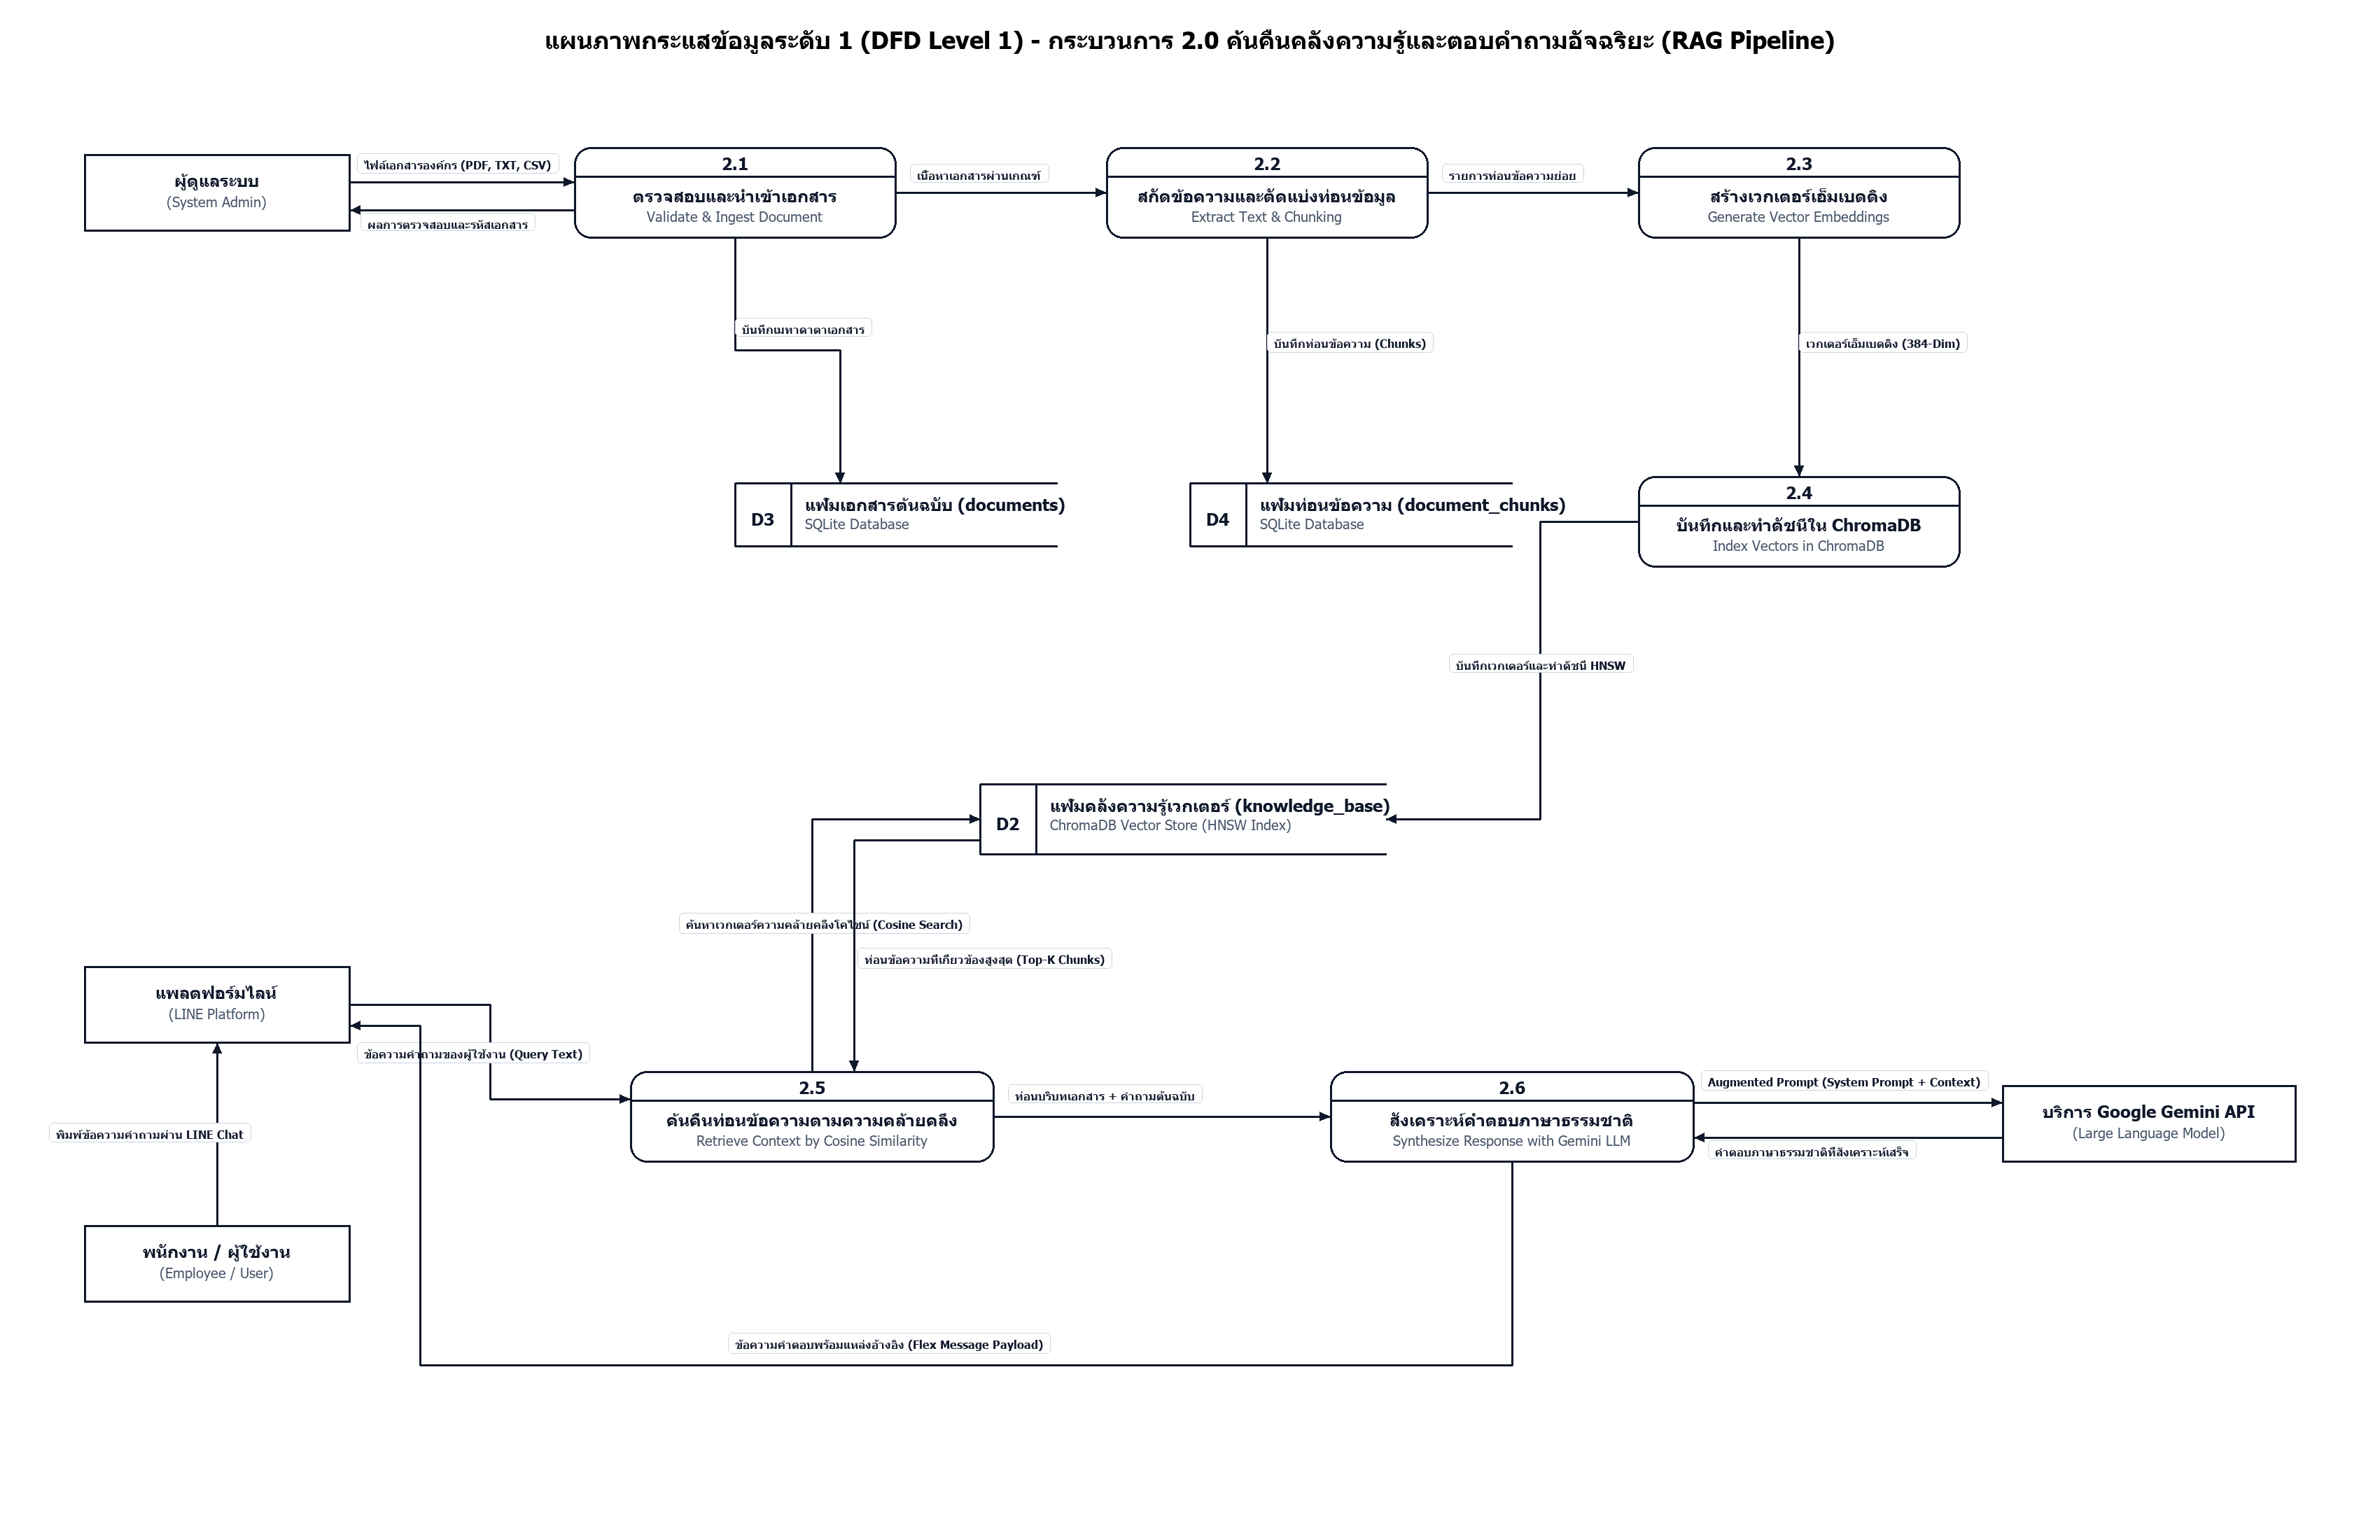
\includegraphics[width=0.95\textwidth]{Image/fig3_3_dfd_level1.png}
\caption{Data Flow Diagram Level 1 ของกระบวนการ 2.0 สืบค้นคลังความรู้และประมวลผลคำถาม}
\label{fig3:dfd1_rag}
\end{figure}

\hspace*{1.3em}
กระบวนการย่อยใน DFD Level 1 ของระบบคลังความรู้ RAG ประกอบด้วย:
\begin{enumerate}[leftmargin=3.5em]
\item[2.1] ตรวจสอบและนำเข้าเอกสาร (Validate \& Ingest Document) ทำหน้าที่ตรวจสอบความถูกต้อง ประเภท และขนาดของไฟล์เอกสารองค์กร บันทึกเมทาดาตาลงในแฟ้ม documents (D3)
\item[2.2] สกัดข้อความและตัดแบ่งท่อนข้อมูล (Extract Text \& Chunking) ทำหน้าที่อ่านเนื้อหาและแบ่งท่อนข้อความตามขนาดที่กำหนด (Chunk Size 800) บันทึกลงในแฟ้ม document\_chunks (D4)
\item[2.3] สร้างเวกเตอร์เอ็มเบดดิง (Generate Vector Embeddings) ทำหน้าที่แปลงท่อนข้อความย่อยเป็นเวกเตอร์ตัวเลขความหนาแน่นสูง (Dense Embeddings 384 มิติ) ด้วยโมเดล BAAI-bge
\item[2.4] บันทึกและทำดัชนีใน ChromaDB (Index Vectors in ChromaDB) ทำหน้าที่จัดเก็บเวกเตอร์และสร้างดัชนีแบบ HNSW ลงในแฟ้มคลังความรู้เวกเตอร์ knowledge\_base (D2)
\item[2.5] ค้นคืนท่อนข้อความตามความคล้ายคลึง (Retrieve Context by Cosine Similarity) ทำหน้าที่รับข้อความคำถามจาก LINE แปลงเป็นเวกเตอร์ และค้นคืนชิ้นส่วนข้อความที่มีความคล้ายคลึงสูงสุด (Top-K Chunks) จาก D2
\item[2.6] สังเคราะห์คำตอบภาษาธรรมชาติ (Synthesize Response with Gemini LLM) ทำหน้าที่ประกอบ Augmented Prompt ส่งไปยัง Google Gemini API และจัดรูปแบบคำตอบส่งกลับสู่ผู้ใช้
\end{enumerate}

\subsection{แหล่งจัดเก็บข้อมูลของระบบ (Data Store Specifications)}
\hspace*{1.3em}
แหล่งจัดเก็บข้อมูลของระบบที่ปรากฏในแผนภาพกระแสข้อมูล ประกอบด้วย 6 แหล่งจัดเก็บข้อมูลหลัก ดังแสดงในตารางที่ 3-4:

\begin{table}[htbp]
\centering
\caption{แหล่งจัดเก็บข้อมูล (Data Store) ของระบบ}
\label{tab3:datastores}
\begin{tabularx}{\textwidth}{| c | c | c | L |}
\hline
\textbf{รหัส} & \textbf{ชื่อ Data Store} & \textbf{ประเภท} & \textbf{คำอธิบายข้อมูลที่จัดเก็บ} \\ \hline
D1 & users & SQLite & ข้อมูลผู้ใช้งานระบบ รหัสผ่านแฮช บทบาท อีเมล และ LINE User ID \\ \hline
D2 & knowledge\_base & ChromaDB & ฐานข้อมูลเวกเตอร์เอ็มเบดดิงและท่อนข้อความสำหรับสืบค้นความคล้ายคลึง \\ \hline
D3 & drive\_logs & SQLite & บันทึกประวัติไฟล์เอกสารต้นฉบับ บัญชีผู้ส่ง และลิงก์ Google Drive \\ \hline
D4 & leave\_requests & SQLite & ข้อมูลคำขอลางาน ประเภทการลา วันที่ขอลา เหตุผล และสถานะการอนุมัติ \\ \hline
D5 & user\_leave\_quotas & SQLite & ข้อมูลโควตาวันลาและสถิติยอดวันลาคงเหลือของพนักงานแต่ละคน \\ \hline
D6 & audit\_logs & SQLite & บันทึกประวัติการเข้าใช้งาน ประวัติการสนทนา และกิจกรรมความปลอดภัย \\ \hline
\end{tabularx}
\end{table}

\clearpage
\section{การกำหนดลักษณะการประมวลผล (Process Specification : PSPEC)}
\hspace*{1.3em}
การกำหนดลักษณะการประมวลผล (Process Specification: PSPEC) ทำหน้าที่อธิบายตรรกะและขั้นตอนการทำงานของกระบวนการย่อยใน DFD อย่างละเอียด โดยระบุรหัสกระบวนการ ชื่อกระบวนการ ข้อมูลนำเข้า ข้อมูลส่งออก และขั้นตอนการทำงาน (Logic) ดังแสดงในตารางที่ 3-5 ถึงตารางที่ 3-16:

\begin{table}[htbp]
\centering
\caption{Process Specification: Process 1.1 ตรวจสอบการเข้าสู่ระบบ}
\label{tab3:pspec1_1}
\begin{tabularx}{\textwidth}{| c | L |}
\hline
\textbf{หัวข้อ} & \textbf{รายละเอียด} \\ \hline
รหัสกระบวนการ & 1.1 \\ \hline
ชื่อกระบวนการ & ตรวจสอบการเข้าสู่ระบบ (Authenticate User Login) \\ \hline
ข้อมูลนำเข้า (Input) & ชื่อผู้ใช้หรืออีเมล (username/email), รหัสผ่าน (password) \\ \hline
ข้อมูลส่งออก (Output) & สถานะการเข้าสู่ระบบ, JWT Session Token, ข้อความแจ้งเตือนความผิดพลาด \\ \hline
ตรรกะการประมวลผล & 1. รับค่าชื่อผู้ใช้และรหัสผ่านจากฟอร์มหน้าเว็บ \newline
2. ค้นหาข้อมูลผู้ใช้ในตาราง users (D1) ด้วย username หรือ email \newline
3. หากไม่พบข้อมูล ให้ส่งรหัสข้อผิดพลาด "ไม่พบบัญชีผู้ใช้งาน" \newline
4. ตรวจสอบรหัสผ่านด้วยฟังก์ชัน BCrypt.checkpw() \newline
5. หากรหัสผ่านถูกต้อง สร้าง JWT Token และบันทึกประวัติการเข้าใช้งานลง audit\_logs \newline
6. ส่งผลลัพธ์พร้อม Token กลับไปยังเบราว์เซอร์เพื่อบันทึก Session \\ \hline
\end{tabularx}
\end{table}

\begin{table}[htbp]
\centering
\caption{Process Specification: Process 1.2 เข้าสู่ระบบด้วย Google OAuth 2.0 และผูกบัญชี LINE}
\label{tab3:pspec1_2}
\begin{tabularx}{\textwidth}{| c | L |}
\hline
\textbf{หัวข้อ} & \textbf{รายละเอียด} \\ \hline
รหัสกระบวนการ & 1.2 \\ \hline
ชื่อกระบวนการ & เข้าสู่ระบบด้วย Google OAuth และผูกบัญชี LINE (Authenticate via Google OAuth & LINE Link) \\ \hline
ข้อมูลนำเข้า (Input) & Authorization Code จาก LINE Platform, State Token \\ \hline
ข้อมูลส่งออก (Output) & เซสชันผู้ใช้งาน, LINE Profile Data, หน้าจอปลายทางตามบทบาท \\ \hline
ตรรกะการประมวลผล & 1. ตรวจสอบความถูกต้องของ State Token เพื่อป้องกัน CSRF \newline
2. นำ Authorization Code ไปแลก Access Token กับ LINE OAuth Server \newline
3. เรียกขอข้อมูลโปรไฟล์ (userId, displayName, pictureUrl) จาก LINE API \newline
4. ตรวจสอบว่า line\_user\_id มีอยู่ในตาราง users (D1) แล้วหรือไม่ \newline
5. หากมี ให้สร้างเซสชันและนำทางเข้าสู่ระบบทันที \newline
6. หากยังไม่มี ให้นำทางไปยังหน้าผูกบัญชีหรือลงทะเบียนสมาชิกใหม่ \\ \hline
\end{tabularx}
\end{table}

\begin{table}[htbp]
\centering
\caption{Process Specification: Process 1.3 จัดการโปรไฟล์และสิทธิ์ผู้ใช้งาน}
\label{tab3:pspec1_3}
\begin{tabularx}{\textwidth}{| c | L |}
\hline
\textbf{หัวข้อ} & \textbf{รายละเอียด} \\ \hline
รหัสกระบวนการ & 1.3 \\ \hline
ชื่อกระบวนการ & จัดการโปรไฟล์และสิทธิ์ผู้ใช้ (Manage Profile and Roles) \\ \hline
ข้อมูลนำเข้า (Input) & รหัสผู้ใช้ (user\_id), ข้อมูลโปรไฟล์ที่แก้ไข, บทบาทสิทธิ์ (Role) \\ \hline
ข้อมูลส่งออก (Output) & ผลการอัปเดตข้อมูลโปรไฟล์ (สำเร็จ / ล้มเหลว) \\ \hline
ตรรกะการประมวลผล & 1. ตรวจสอบสิทธิ์ของผู้ดำเนินการว่ามีสิทธิ์แก้ไขหรือไม่ (Admin หรือเจ้าของบัญชี) \newline
2. ตรวจสอบความถูกต้องของรูปแบบข้อมูล (Data Validation) เช่น รูปแบบอีเมล \newline
3. อัปเดตข้อมูลลงตาราง users (D1) \newline
4. บันทึกประวัติการแก้ไขข้อมูลลงในระบบ audit\_logs \\ \hline
\end{tabularx}
\end{table}

\begin{table}[htbp]
\centering
\caption{Process Specification: Process 2.1 ตรวจสอบและนำเข้าไฟล์เอกสาร}
\label{tab3:pspec2_1}
\begin{tabularx}{\textwidth}{| c | L |}
\hline
\textbf{หัวข้อ} & \textbf{รายละเอียด} \\ \hline
รหัสกระบวนการ & 2.1 \\ \hline
ชื่อกระบวนการ & ตรวจสอบและนำเข้าไฟล์เอกสาร (Validate and Ingest Document) \\ \hline
ข้อมูลนำเข้า (Input) & ไฟล์เอกสาร (PDF, TXT, CSV, DOCX), รหัสองค์กร (org\_id) \\ \hline
ข้อมูลส่งออก (Output) & ข้อมูลเมทาดาตาของเอกสาร (Document Metadata), ข้อความแจ้งสถานะ \\ \hline
ตรรกะการประมวลผล & 1. ตรวจสอบนามสกุลและ MIME Type ของไฟล์ว่าอยู่ในประเภทที่รองรับหรือไม่ \newline
2. ตรวจสอบขนาดไฟล์ไม่เกิน 25 MB \newline
3. คำนวณค่าแฮช SHA-256 ของเนื้อไฟล์เพื่อป้องกันการอัปโหลดไฟล์ซ้ำ \newline
4. บันทึกข้อมูลไฟล์ลงในตาราง documents (D3) และส่งต่อเข้าคิวสกัดข้อความ \\ \hline
\end{tabularx}
\end{table}

\begin{table}[htbp]
\centering
\caption{Process Specification: Process 2.2 สกัดข้อความและตัดแบ่งท่อนข้อมูล}
\label{tab3:pspec2_2}
\begin{tabularx}{\textwidth}{| c | L |}
\hline
\textbf{หัวข้อ} & \textbf{รายละเอียด} \\ \hline
รหัสกระบวนการ & 2.2 \\ \hline
ชื่อกระบวนการ & สกัดข้อความและตัดแบ่งท่อนข้อมูล (Extract Text and Chunking) \\ \hline
ข้อมูลนำเข้า (Input) & ไฟล์เอกสารต้นฉบับจากคลังเอกสาร (D3) \\ \hline
ข้อมูลส่งออก (Output) & ท่อนข้อความย่อย (Document Chunks) พร้อมข้อมูลบริบทอ้างอิง \\ \hline
ตรรกะการประมวลผล & 1. อ่านเนื้อหาข้อความจากไฟล์ตามประเภท (PyPDF สำหรับ PDF, Text loader สำหรับ TXT) \newline
2. ทำความสะอาดข้อความ ลบอักขระพิเศษที่ไม่จำเป็นและช่องว่างซ้ำซ้อน \newline
3. ตัดแบ่งข้อความเป็นท่อนย่อย (Chunk Size = 800 ตัวอักษร, Chunk Overlap = 100 ตัวอักษร) \newline
4. ผูกหมายเลขหน้าและรหัสเอกสารเข้ากับแต่ละท่อนข้อความ \newline
5. บันทึกท่อนข้อความลงในตาราง document\_chunks (D4) \\ \hline
\end{tabularx}
\end{table}

\begin{table}[htbp]
\centering
\caption{Process Specification: Process 2.3 สร้างเวกเตอร์เอ็มเบดดิง}
\label{tab3:pspec2_3}
\begin{tabularx}{\textwidth}{| c | L |}
\hline
\textbf{หัวข้อ} & \textbf{รายละเอียด} \\ \hline
รหัสกระบวนการ & 2.3 \\ \hline
ชื่อกระบวนการ & สร้างเวกเตอร์เอ็มเบดดิง (Generate Vector Embeddings) \\ \hline
ข้อมูลนำเข้า (Input) & ท่อนข้อความย่อย (Document Chunks) จาก D4 \\ \hline
ข้อมูลส่งออก (Output) & เวกเตอร์ตัวเลขหลายมิติ (Dense Vector Embeddings) \\ \hline
ตรรกะการประมวลผล & 1. รับรายการท่อนข้อความย่อยเข้าสู่โมเดล FastEmbed / BAAI-bge \newline
2. แปลงข้อความเป็นเวกเตอร์ตัวเลขที่มีขนาดมิติคงที่ (Dimension = 384 หรือ 768) \newline
3. ตรวจสอบความสมบูรณ์ของเวกเตอร์ (ไม่มีค่าว่างหรือ NaN) \newline
4. ส่งผลลัพธ์เวกเตอร์พร้อมเมทาดาตาไปยังกระบวนการบันทึกลงฐานข้อมูลเวกเตอร์ \\ \hline
\end{tabularx}
\end{table}

\begin{table}[htbp]
\centering
\caption{Process Specification: Process 2.4 บันทึกและทำดัชนีเวกเตอร์ใน ChromaDB}
\label{tab3:pspec2_4}
\begin{tabularx}{\textwidth}{| c | L |}
\hline
\textbf{หัวข้อ} & \textbf{รายละเอียด} \\ \hline
รหัสกระบวนการ & 2.4 \\ \hline
ชื่อกระบวนการ & บันทึกและดัชนีเวกเตอร์ (Index Vectors in ChromaDB) \\ \hline
ข้อมูลนำเข้า (Input) & เวกเตอร์ตัวเลข, รหัสท่อนข้อความ (chunk\_id), เมทาดาตา (org\_id, doc\_id) \\ \hline
ข้อมูลส่งออก (Output) & สถานะการบันทึกสำเร็จ, ดัชนีเวกเตอร์ที่พร้อมใช้งาน \\ \hline
ตรรกะการประมวลผล & 1. เปิดการเชื่อมต่อกับ ChromaDB Client \newline
2. เข้าถึงคอลเลกชัน (Collection) ที่ตรงกับรหัสองค์กร (Multi-Tenant Collection) \newline
3. บันทึกเวกเตอร์ ข้อความต้นฉบับ และเมทาดาตาลงในคอลเลกชัน \newline
4. สร้างดัชนี HNSW (Hierarchical Navigable Small World) เพื่อความรวดเร็วในการค้นหา \newline
5. อัปเดตสถานะเอกสารในตาราง documents (D3) เป็น 'READY' \\ \hline
\end{tabularx}
\end{table}

\begin{table}[htbp]
\centering
\caption{Process Specification: Process 2.5 ค้นคืนท่อนข้อความตามความคล้ายคลึง}
\label{tab3:pspec2_5}
\begin{tabularx}{\textwidth}{| c | L |}
\hline
\textbf{หัวข้อ} & \textbf{รายละเอียด} \\ \hline
รหัสกระบวนการ & 2.5 \\ \hline
ชื่อกระบวนการ & ค้นคืนท่อนข้อความตามความคล้ายคลึง (Retrieve Context by Similarity) \\ \hline
ข้อมูลนำเข้า (Input) & ข้อความคำถามของผู้ใช้ (Query Text), รหัสองค์กร (org\_id) \\ \hline
ข้อมูลส่งออก (Output) & ท่อนข้อความที่เกี่ยวข้องสูงสุด (Top-K Chunks, K = 3 ถึง 5) \\ \hline
ตรรกะการประมวลผล & 1. นำข้อความคำถามมาแปลงเป็นเวกเตอร์ด้วยโมเดล Embedding เดียวกัน \newline
2. ดำเนินการค้นหาใน ChromaDB (D5) ภายใต้คอลเลกชันขององค์กร \newline
3. คำนวณค่าความคล้ายคลึงแบบโคไซน์ (Cosine Similarity Score) \newline
4. กรองเฉพาะท่อนข้อความที่มีคะแนนเกินเกณฑ์ขั้นต่ำ (Threshold >= 0.65) \newline
5. ส่งคืนท่อนข้อความที่มีความคล้ายคลึงสูงสุด 3-5 รายการแรกพร้อมคะแนน \\ \hline
\end{tabularx}
\end{table}

\begin{table}[htbp]
\centering
\caption{Process Specification: Process 2.6 สังเคราะห์คำตอบด้วย Google Gemini}
\label{tab3:pspec2_6}
\begin{tabularx}{\textwidth}{| c | L |}
\hline
\textbf{หัวข้อ} & \textbf{รายละเอียด} \\ \hline
รหัสกระบวนการ & 2.6 \\ \hline
ชื่อกระบวนการ & สังเคราะห์คำตอบภาษาธรรมชาติ (Synthesize Response with LLM) \\ \hline
ข้อมูลนำเข้า (Input) & คำถามของผู้ใช้, ท่อนข้อความบริบทที่ค้นคืนได้ (Retrieved Chunks), System Prompt \\ \hline
ข้อมูลส่งออก (Output) & คำตอบภาษาธรรมชาติที่สละสลวย อ้างอิงจากเอกสารองค์กร \\ \hline
ตรรกะการประมวลผล & 1. ประกอบ Augmented Prompt โดยนำท่อนบริบทมาวางต่อจากคำสั่งระบบ (System Prompt) \newline
2. กำหนดเงื่อนไขให้โมเดลตอบเฉพาะข้อมูลที่ปรากฏในบริบท หากไม่มีให้ตอบอย่างสุภาพว่าไม่พบข้อมูล \newline
3. ส่งคำขอไปยัง Google Gemini API ผ่านการเชื่อมต่อ HTTPS \newline
4. รับข้อความคำตอบและตรวจสอบความสมบูรณ์ของประโยค \newline
5. ส่งข้อความคำตอบต่อไปยังกระบวนการจัดรูปแบบและส่งกลับผ่าน LINE \\ \hline
\end{tabularx}
\end{table}

\begin{table}[htbp]
\centering
\caption{Process Specification: Process 3.1 อัปโหลดและจัดระเบียบไฟล์บน Google Drive}
\label{tab3:pspec3_1}
\begin{tabularx}{\textwidth}{| c | L |}
\hline
\textbf{หัวข้อ} & \textbf{รายละเอียด} \\ \hline
รหัสกระบวนการ & 3.1 \\ \hline
ชื่อกระบวนการ & จัดเก็บไฟล์บน Google Drive (Upload and Organize on Drive) \\ \hline
ข้อมูลนำเข้า (Input) & ไฟล์เอกสารหรือรูปภาพ, ข้อมูลผู้ใช้, วันที่ที่ส่ง \\ \hline
ข้อมูลส่งออก (Output) & รหัสไฟล์บน Drive (\texttt{drive\_file\_id}), ลิงก์เข้าถึงเอกสาร (\texttt{drive\_url}) \\ \hline
ตรรกะการประมวลผล & 1. ยืนยันตัวตนกับ Google Cloud Service Account \newline
2. ตรวจสอบโฟลเดอร์ปลายทางตามปีและเดือน (เช่น /2026/10) หากยังไม่มีให้สร้างโฟลเดอร์ใหม่ \newline
3. อัปโหลดไฟล์ขึ้นสู่โฟลเดอร์บน Google Drive \newline
4. บันทึกข้อมูลประวัติไฟล์และลิงก์ลงตาราง drive\_logs (D6) \newline
5. ส่งคืนลิงก์เอกสารให้ผู้ใช้งานตรวจสอบ \\ \hline
\end{tabularx}
\end{table}

\begin{table}[htbp]
\centering
\caption{Process Specification: Process 4.1 ตรวจสอบและรับเหตุการณ์ LINE Webhook}
\label{tab3:pspec4_1}
\begin{tabularx}{\textwidth}{| c | L |}
\hline
\textbf{หัวข้อ} & \textbf{รายละเอียด} \\ \hline
รหัสกระบวนการ & 4.1 \\ \hline
ชื่อกระบวนการ & รับและตรวจสอบ LINE Webhook (Handle LINE Webhook Events) \\ \hline
ข้อมูลนำเข้า (Input) & HTTP Request Body จาก LINE Platform, ส่วนหัว X-Line-Signature \\ \hline
ข้อมูลส่งออก (Output) & รายการเหตุการณ์ (Webhook Events), HTTP 200 OK Response \\ \hline
ตรรกะการประมวลผล & 1. ตรวจสอบลายเซ็นดิจิทัล X-Line-Signature ด้วย Channel Secret และ HMAC-SHA256 \newline
2. หากลายเซ็นไม่ถูกต้อง ให้ปฏิเสธคำขอและส่งรหัส HTTP 400 Bad Request \newline
3. แยกวิเคราะห์ JSON Payload ออกเป็นรายการ Event แต่ละรายการ \newline
4. ตรวจสอบประเภท Event (MessageEvent, FollowEvent, PostbackEvent) \newline
5. ส่งต่อข้อความไปยังกระบวนการประมวลผลคลังความรู้ RAG หรือคำสั่งที่เกี่ยวข้อง \\ \hline
\end{tabularx}
\end{table}

\begin{table}[htbp]
\centering
\caption{Process Specification: Process 4.2 จัดโครงสร้างและส่งกลับ LINE Flex Message}
\label{tab3:pspec4_2}
\begin{tabularx}{\textwidth}{| c | L |}
\hline
\textbf{หัวข้อ} & \textbf{รายละเอียด} \\ \hline
รหัสกระบวนการ & 4.2 \\ \hline
ชื่อกระบวนการ & จัดรูปแบบและตอบกลับ Flex Message (Format and Reply Flex Message) \\ \hline
ข้อมูลนำเข้า (Input) & ข้อความคำตอบ, ลิงก์อ้างอิง, ข้อมูลสินค้า, Reply Token \\ \hline
ข้อมูลส่งออก (Output) & LINE Flex Message JSON Payload, สถานะการส่งสำเร็จ \\ \hline
ตรรกะการประมวลผล & 1. สร้างโครงสร้าง Bubble Container ตามรูปแบบมาตรฐาน LINE Flex Message \newline
2. ใส่รูปภาพประกอบ หัวข้อข้อความ รายละเอียดคำตอบ และปุ่มทางลัดไปยังลิงก์ที่เกี่ยวข้อง \newline
3. เรียกใช้ LINE Messaging API method replyMessage ด้วย Reply Token \newline
4. ตรวจสอบการตอบสนองจาก LINE API และบันทึกประวัติการส่งข้อความ \\ \hline
\end{tabularx}
\end{table}

\section{พจนานุกรมข้อมูล (Data Flow Dictionary)}
\hspace*{1.3em}
พจนานุกรมข้อมูลทำหน้าที่อธิบายรายละเอียดของกระแสข้อมูล (Data Flow) ทุกเส้นที่เชื่อมโยงระหว่างเอนทิตีภายนอก กระบวนการ และแหล่งจัดเก็บข้อมูลในระบบ โดยระบุชื่อกระแสข้อมูล คำอธิบาย แหล่งกำเนิด กระบวนการ ปลายทาง และโครงสร้างข้อมูล ดังแสดงในตารางที่ 3-17 ถึงตารางที่ 3-26:

\begin{table}[htbp]
\centering
\caption{Data Dictionary: ข้อมูลการเข้าสู่ระบบ (Login Credentials)}
\label{tab3:df_login}
\begin{tabularx}{\textwidth}{| c | L |}
\hline
\textbf{หัวข้อ} & \textbf{รายละเอียด} \\ \hline
ชื่อกระแสข้อมูล & ข้อมูลการเข้าสู่ระบบ (Login Credentials) \\ \hline
คำอธิบาย & ข้อมูลที่ผู้ใช้งานป้อนเพื่อขอยืนยันตัวตนเข้าสู่ระบบเว็บแอปพลิเคชัน \\ \hline
แหล่งกำเนิด (Source) & ผู้ใช้งาน (Admin / Employee) \\ \hline
กระบวนการ (Process) & 1.1 ตรวจสอบการเข้าสู่ระบบ \\ \hline
ปลายทาง (Destination) & ฐานข้อมูล D1: users \\ \hline
โครงสร้างข้อมูล & username + password + [line\_user\_id] + timestamp + ip\_address \\ \hline
\end{tabularx}
\end{table}

\begin{table}[htbp]
\centering
\caption{Data Dictionary: โทเค็นและเซสชันผู้ใช้งาน (Authentication Token)}
\label{tab3:df_token}
\begin{tabularx}{\textwidth}{| c | L |}
\hline
\textbf{หัวข้อ} & \textbf{รายละเอียด} \\ \hline
ชื่อกระแสข้อมูล & โทเค็นยืนยันตัวตน (Authentication Token \& Session Data) \\ \hline
คำอธิบาย & ข้อมูลการรับรองความถูกต้องของเซสชันที่สร้างขึ้นหลังผ่านการยืนยันตัวตนสำเร็จ \\ \hline
แหล่งกำเนิด (Source) & กระบวนการ 1.1 หรือ 1.2 \\ \hline
กระบวนการ (Process) & 1.0 ตรวจสอบสิทธิ์และจัดการผู้ใช้งาน \\ \hline
ปลายทาง (Destination) & เบราว์เซอร์ผู้ใช้งาน (Web Client Session Storage / Cookie) \\ \hline
โครงสร้างข้อมูล & jwt\_token + user\_id + username + role + org\_id + expires\_at \\ \hline
\end{tabularx}
\end{table}

\begin{table}[htbp]
\centering
\caption{Data Dictionary: ข้อมูลโปรไฟล์ผู้ใช้งาน (User Profile Data)}
\label{tab3:df_profile}
\begin{tabularx}{\textwidth}{| c | L |}
\hline
\textbf{หัวข้อ} & \textbf{รายละเอียด} \\ \hline
ชื่อกระแสข้อมูล & ข้อมูลโปรไฟล์ผู้ใช้งาน (User Profile Data) \\ \hline
คำอธิบาย & ข้อมูลส่วนบุคคลของผู้ใช้งานในระบบ เช่น ชื่อ-นามสกุล อีเมล บทบาท และสถานะ \\ \hline
แหล่งกำเนิด (Source) & ผู้ใช้งาน หรือ ผู้ดูแลระบบ \\ \hline
กระบวนการ (Process) & 1.3 จัดการโปรไฟล์และสิทธิ์ผู้ใช้งาน \\ \hline
ปลายทาง (Destination) & ฐานข้อมูล D1: users \\ \hline
โครงสร้างข้อมูล & user\_id + username + display\_name + email + role + org\_id + updated\_at \\ \hline
\end{tabularx}
\end{table}

\begin{table}[htbp]
\centering
\caption{Data Dictionary: ไฟล์เอกสารคลังความรู้ (Knowledge Documents)}
\label{tab3:df_doc}
\begin{tabularx}{\textwidth}{| c | L |}
\hline
\textbf{หัวข้อ} & \textbf{รายละเอียด} \\ \hline
ชื่อกระแสข้อมูล & ไฟล์เอกสารคลังความรู้ (Knowledge Documents Payload) \\ \hline
คำอธิบาย & ไฟล์คู่มือสินค้า นโยบายบริษัท และระเบียบปฏิบัติที่อัปโหลดเข้าสู่ระบบ RAG \\ \hline
แหล่งกำเนิด (Source) & ผู้ดูแลระบบ (Admin ผ่านหน้าจัดการคลังความรู้) \\ \hline
กระบวนการ (Process) & 2.1 ตรวจสอบและนำเข้าไฟล์เอกสาร \\ \hline
ปลายทาง (Destination) & ฐานข้อมูล D3: documents และระบบจัดเก็บไฟล์ในเซิร์ฟเวอร์ \\ \hline
โครงสร้างข้อมูล & doc\_id + file\_name + file\_bytes + file\_type + file\_size + file\_hash + upload\_date \\ \hline
\end{tabularx}
\end{table}

\begin{table}[htbp]
\centering
\caption{Data Dictionary: ท่อนข้อความที่สกัดได้ (Document Chunks)}
\label{tab3:df_chunks}
\begin{tabularx}{\textwidth}{| c | L |}
\hline
\textbf{หัวข้อ} & \textbf{รายละเอียด} \\ \hline
ชื่อกระแสข้อมูล & ท่อนข้อความที่สกัดได้ (Document Chunks) \\ \hline
คำอธิบาย & เนื้อหาข้อความย่อยที่ผ่านการทำความสะอาดและตัดแบ่งตามขนาดที่กำหนด \\ \hline
แหล่งกำเนิด (Source) & กระบวนการ 2.2 สกัดข้อความและตัดแบ่งท่อนข้อมูล \\ \hline
กระบวนการ (Process) & 2.3 สร้างเวกเตอร์เอ็มเบดดิง \\ \hline
ปลายทาง (Destination) & ฐานข้อมูล D4: document\_chunks \\ \hline
โครงสร้างข้อมูล & chunk\_id + doc\_id + chunk\_index + chunk\_text + page\_number + char\_length \\ \hline
\end{tabularx}
\end{table}

\begin{table}[htbp]
\centering
\caption{Data Dictionary: เวกเตอร์เอ็มเบดดิง (Embedding Vectors)}
\label{tab3:df_vectors}
\begin{tabularx}{\textwidth}{| c | L |}
\hline
\textbf{หัวข้อ} & \textbf{รายละเอียด} \\ \hline
ชื่อกระแสข้อมูล & เวกเตอร์เอ็มเบดดิง (Dense Embedding Vectors) \\ \hline
คำอธิบาย & เวกเตอร์ตัวเลขหลายมิติที่แทนความหมายเชิงบริบทของท่อนข้อความ \\ \hline
แหล่งกำเนิด (Source) & กระบวนการ 2.3 สร้างเวกเตอร์เอ็มเบดดิง (FastEmbed) \\ \hline
กระบวนการ (Process) & 2.4 บันทึกและทำดัชนีเวกเตอร์ใน ChromaDB \\ \hline
ปลายทาง (Destination) & ฐานข้อมูลเวกเตอร์ D5: vector\_store (ChromaDB) \\ \hline
โครงสร้างข้อมูล & vector\_id + chunk\_id + org\_id + float\_array[384] + metadata\_json \\ \hline
\end{tabularx}
\end{table}

\begin{table}[htbp]
\centering
\caption{Data Dictionary: ข้อความคำถามของผู้ใช้งาน (User Question Payload)}
\label{tab3:df_question}
\begin{tabularx}{\textwidth}{| c | L |}
\hline
\textbf{หัวข้อ} & \textbf{รายละเอียด} \\ \hline
ชื่อกระแสข้อมูล & ข้อความคำถามของผู้ใช้งาน (User Question Payload) \\ \hline
คำอธิบาย & ข้อความภาษาธรรมชาติที่พนักงานพิมพ์สอบถามข้อมูลสินค้าหรือระเบียบผ่าน LINE \\ \hline
แหล่งกำเนิด (Source) & แพลตฟอร์ม LINE (LINE Messaging API Webhook) \\ \hline
กระบวนการ (Process) & 4.1 ตรวจสอบและรับเหตุการณ์ LINE Webhook \\ \hline
ปลายทาง (Destination) & กระบวนการ 2.5 ค้นคืนท่อนข้อความตามความคล้ายคลึง \\ \hline
โครงสร้างข้อมูล & line\_user\_id + message\_id + query\_text + timestamp + reply\_token \\ \hline
\end{tabularx}
\end{table}

\begin{table}[htbp]
\centering
\caption{Data Dictionary: บริบทเอกสารที่ค้นคืนได้ (Retrieved Context)}
\label{tab3:df_context}
\begin{tabularx}{\textwidth}{| c | L |}
\hline
\textbf{หัวข้อ} & \textbf{รายละเอียด} \\ \hline
ชื่อกระแสข้อมูล & บริบทเอกสารที่ค้นคืนได้ (Retrieved Context Chunks) \\ \hline
คำอธิบาย & รายการท่อนข้อความที่มีคะแนนความคล้ายคลึงสูงสุดที่ดึงมาจาก ChromaDB \\ \hline
แหล่งกำเนิด (Source) & ฐานข้อมูลเวกเตอร์ D5: vector\_store \\ \hline
กระบวนการ (Process) & 2.6 สังเคราะห์คำตอบด้วย Google Gemini \\ \hline
ปลายทาง (Destination) & โมเดลภาษาขนาดใหญ่ Google Gemini API \\ \hline
โครงสร้างข้อมูล & array\_of\_chunks[chunk\_text + similarity\_score + doc\_name + page\_num] \\ \hline
\end{tabularx}
\end{table}

\begin{table}[htbp]
\centering
\caption{Data Dictionary: คำตอบภาษาธรรมชาติจาก AI (AI Synthesized Answer)}
\label{tab3:df_ai_answer}
\begin{tabularx}{\textwidth}{| c | L |}
\hline
\textbf{หัวข้อ} & \textbf{รายละเอียด} \\ \hline
ชื่อกระแสข้อมูล & คำตอบภาษาธรรมชาติจาก AI (AI Synthesized Answer) \\ \hline
คำอธิบาย & ข้อความคำตอบที่โมเดลภาษาขนาดใหญ่สร้างขึ้นโดยอ้างอิงจากบริบทเอกสารจริง \\ \hline
แหล่งกำเนิด (Source) & Google Gemini 1.5 Flash API \\ \hline
กระบวนการ (Process) & 4.2 จัดโครงสร้างและส่งกลับ LINE Flex Message \\ \hline
ปลายทาง (Destination) & กระบวนการตอบกลับข้อความ \\ \hline
โครงสร้างข้อมูล & generated\_answer\_text + confidence\_level + source\_citations + processing\_time \\ \hline
\end{tabularx}
\end{table}

\begin{table}[htbp]
\centering
\caption{Data Dictionary: ข้อความตอบกลับ Flex Message (LINE Flex Message Payload)}
\label{tab3:df_flex_reply}
\begin{tabularx}{\textwidth}{| c | L |}
\hline
\textbf{หัวข้อ} & \textbf{รายละเอียด} \\ \hline
ชื่อกระแสข้อมูล & ข้อความตอบกลับ Flex Message (LINE Flex Message Payload) \\ \hline
คำอธิบาย & ชุดข้อมูลการ์ดข้อความพร้อมรูปแบบ UI และปุ่มแอ็กชันส่งกลับไปยังแชท LINE \\ \hline
แหล่งกำเนิด (Source) & กระบวนการ 4.2 จัดโครงสร้างและส่งกลับ LINE Flex Message \\ \hline
กระบวนการ (Process) & 4.0 เชื่อมต่อและสื่อสารผ่านแพลตฟอร์ม LINE \\ \hline
ปลายทาง (Destination) & ผู้ใช้งาน LINE (พนักงาน บริษัท ฮาร์ทวอมมิ่ง จำกัด) \\ \hline
โครงสร้างข้อมูล & reply\_token + flex\_container\_json[header, hero\_image, body, footer\_buttons] \\ \hline
\end{tabularx}
\end{table}

\section{การออกแบบข้อมูล (Data Element Description)}
\hspace*{1.3em}
การออกแบบข้อมูล (Data Element Description) เป็นการอธิบายคุณลักษณะเฉพาะของตัวแปรหรือฟิลด์ข้อมูลแต่ละตัวในระบบ เช่น รหัสข้อมูล ชนิดข้อมูล ขนาด รูปแบบ และตารางที่สังกัด ดังแสดงในตารางที่ 3-27 ถึงตารางที่ 3-42:

\begin{table}[htbp]
\centering
\caption{Data Element Description: รหัสผู้ใช้งาน (id)}
\label{tab3:de_id}
\begin{tabularx}{\textwidth}{| c | L |}
\hline
\textbf{หัวข้อ} & \textbf{รายละเอียด} \\ \hline
รหัสรายการข้อมูล & DE-001 \\ \hline
ชื่อรายการข้อมูล & รหัสผู้ใช้งาน (id) \\ \hline
คำอธิบาย & ตัวเลขรหัสประจำตัวของผู้ใช้งานในระบบ สร้างอัตโนมัติ (Primary Key) \\ \hline
ชนิดข้อมูล (Data Type) & Integer \\ \hline
ความยาว (Length) & - \\ \hline
รูปแบบข้อมูล (Data Format) & ตัวเลขจำนวนเต็มบวก \\ \hline
ตารางข้อมูล (Table) & users (D1) \\ \hline
\end{tabularx}
\end{table}

\begin{table}[htbp]
\centering
\caption{Data Element Description: ชื่อบัญชีผู้ใช้งาน (username)}
\label{tab3:de_username}
\begin{tabularx}{\textwidth}{| c | L |}
\hline
\textbf{หัวข้อ} & \textbf{รายละเอียด} \\ \hline
รหัสรายการข้อมูล & DE-002 \\ \hline
ชื่อรายการข้อมูล & ชื่อบัญชีผู้ใช้งาน (username) \\ \hline
คำอธิบาย & ชื่อบัญชีสำหรับเข้าสู่ระบบ มีค่าไม่ซ้ำกันในระบบ \\ \hline
ชนิดข้อมูล (Data Type) & Varchar \\ \hline
ความยาว (Length) & 50 \\ \hline
รูปแบบข้อมูล (Data Format) & ตัวอักษรภาษาอังกฤษและตัวเลข เช่น user01 \\ \hline
ตารางข้อมูล (Table) & users (D1) \\ \hline
\end{tabularx}
\end{table}

\begin{table}[htbp]
\centering
\caption{Data Element Description: อีเมล (email)}
\label{tab3:de_email}
\begin{tabularx}{\textwidth}{| c | L |}
\hline
\textbf{หัวข้อ} & \textbf{รายละเอียด} \\ \hline
รหัสรายการข้อมูล & DE-003 \\ \hline
ชื่อรายการข้อมูล & อีเมลผู้ใช้งาน (email) \\ \hline
คำอธิบาย & อีเมลสำหรับติดต่อ กู้คืนรหัสผ่าน และการแจ้งเตือน \\ \hline
ชนิดข้อมูล (Data Type) & Varchar \\ \hline
ความยาว (Length) & 100 \\ \hline
รูปแบบข้อมูล (Data Format) & รูปแบบอีเมลมาตรฐาน เช่น employee@heartwarming.co.th \\ \hline
ตารางข้อมูล (Table) & users (D1) \\ \hline
\end{tabularx}
\end{table}

\begin{table}[htbp]
\centering
\caption{Data Element Description: รหัสผ่านที่แฮช (password\_hash)}
\label{tab3:de_pwd}
\begin{tabularx}{\textwidth}{| c | L |}
\hline
\textbf{หัวข้อ} & \textbf{รายละเอียด} \\ \hline
รหัสรายการข้อมูล & DE-004 \\ \hline
ชื่อรายการข้อมูล & รหัสผ่านที่ผ่านการแฮช (password\_hash) \\ \hline
คำอธิบาย & ข้อความรหัสผ่านที่ผ่านการเข้ารหัสทางเดียวด้วยอัลกอริทึม BCrypt \\ \hline
ชนิดข้อมูล (Data Type) & Varchar \\ \hline
ความยาว (Length) & 255 \\ \hline
รูปแบบข้อมูล (Data Format) & ข้อความสตริงแฮช 60 ตัวอักษร เช่น \$2b\$12\$e8X... \\ \hline
ตารางข้อมูล (Table) & users (D1) \\ \hline
\end{tabularx}
\end{table}

\begin{table}[htbp]
\centering
\caption{Data Element Description: รหัสบัญชี LINE (line\_user\_id)}
\label{tab3:de_line_id}
\begin{tabularx}{\textwidth}{| c | L |}
\hline
\textbf{หัวข้อ} & \textbf{รายละเอียด} \\ \hline
รหัสรายการข้อมูล & DE-005 \\ \hline
ชื่อรายการข้อมูล & รหัสประจำตัวผู้ใช้บน LINE (line\_user\_id) \\ \hline
คำอธิบาย & รหัสเฉพาะที่ออกโดยแพลตฟอร์ม LINE สำหรับระบุตัวตนของผู้ใช้ \\ \hline
ชนิดข้อมูล (Data Type) & Varchar \\ \hline
ความยาว (Length) & 64 \\ \hline
รูปแบบข้อมูล (Data Format) & ตัวอักษรและตัวเลขขึ้นต้นด้วย U เช่น U1234567890abcdef... \\ \hline
ตารางข้อมูล (Table) & users (D1) \\ \hline
\end{tabularx}
\end{table}

\begin{table}[htbp]
\centering
\caption{Data Element Description: ระดับบทบาทและสิทธิ์ (role)}
\label{tab3:de_role}
\begin{tabularx}{\textwidth}{| c | L |}
\hline
\textbf{หัวข้อ} & \textbf{รายละเอียด} \\ \hline
รหัสรายการข้อมูล & DE-006 \\ \hline
ชื่อรายการข้อมูล & ระดับบทบาทสิทธิ์ (role) \\ \hline
คำอธิบาย & ระดับสิทธิ์ในการเข้าถึงและใช้งานระบบตามหลักการ RBAC \\ \hline
ชนิดข้อมูล (Data Type) & Varchar \\ \hline
ความยาว (Length) & 20 \\ \hline
รูปแบบข้อมูล (Data Format) & admin, manager, employee, user \\ \hline
ตารางข้อมูล (Table) & users (D1) \\ \hline
\end{tabularx}
\end{table}

\begin{table}[htbp]
\centering
\caption{Data Element Description: รหัสองค์กร (org\_id)}
\label{tab3:de_org_id}
\begin{tabularx}{\textwidth}{| c | L |}
\hline
\textbf{หัวข้อ} & \textbf{รายละเอียด} \\ \hline
รหัสรายการข้อมูล & DE-007 \\ \hline
ชื่อรายการข้อมูล & รหัสองค์กร (org\_id) \\ \hline
คำอธิบาย & รหัสประจำตัวองค์กรหรือบริษัท สำหรับแยกข้อมูล Multi-Tenant \\ \hline
ชนิดข้อมูล (Data Type) & Integer \\ \hline
ความยาว (Length) & - \\ \hline
รูปแบบข้อมูล (Data Format) & ตัวเลขจำนวนเต็มบวก (เช่น 1 = บริษัท ฮาร์ทวอมมิ่ง จำกัด) \\ \hline
ตารางข้อมูล (Table) & organizations (D2), users (D1), documents (D3) \\ \hline
\end{tabularx}
\end{table}

\begin{table}[htbp]
\centering
\caption{Data Element Description: ชื่อองค์กร (org\_name)}
\label{tab3:de_org_name}
\begin{tabularx}{\textwidth}{| c | L |}
\hline
\textbf{หัวข้อ} & \textbf{รายละเอียด} \\ \hline
รหัสรายการข้อมูล & DE-008 \\ \hline
ชื่อรายการข้อมูล & ชื่อองค์กรหรือบริษัท (org\_name) \\ \hline
คำอธิบาย & ชื่อทางการขององค์กร \\ \hline
ชนิดข้อมูล (Data Type) & Varchar \\ \hline
ความยาว (Length) & 100 \\ \hline
รูปแบบข้อมูล (Data Format) & ข้อความ เช่น บริษัท ฮาร์ทวอมมิ่ง จำกัด \\ \hline
ตารางข้อมูล (Table) & organizations (D2) \\ \hline
\end{tabularx}
\end{table}

\begin{table}[htbp]
\centering
\caption{Data Element Description: รหัสเอกสาร (doc\_id)}
\label{tab3:de_doc_id}
\begin{tabularx}{\textwidth}{| c | L |}
\hline
\textbf{หัวข้อ} & \textbf{รายละเอียด} \\ \hline
รหัสรายการข้อมูล & DE-009 \\ \hline
ชื่อรายการข้อมูล & รหัสเอกสาร (doc\_id) \\ \hline
คำอธิบาย & รหัสประจำตัวเอกสารที่นำเข้าสู่คลังความรู้ RAG \\ \hline
ชนิดข้อมูล (Data Type) & Integer \\ \hline
ความยาว (Length) & - \\ \hline
รูปแบบข้อมูล (Data Format) & ตัวเลขจำนวนเต็มบวก (Auto Increment) \\ \hline
ตารางข้อมูล (Table) & documents (D3), document\_chunks (D4) \\ \hline
\end{tabularx}
\end{table}

\begin{table}[htbp]
\centering
\caption{Data Element Description: ชื่อไฟล์เอกสาร (file\_name)}
\label{tab3:de_file_name}
\begin{tabularx}{\textwidth}{| c | L |}
\hline
\textbf{หัวข้อ} & \textbf{รายละเอียด} \\ \hline
รหัสรายการข้อมูล & DE-010 \\ \hline
ชื่อรายการข้อมูล & ชื่อไฟล์เอกสาร (file\_name) \\ \hline
คำอธิบาย & ชื่อไฟล์เอกสารต้นฉบับที่อัปโหลดเข้าสู่ระบบ \\ \hline
ชนิดข้อมูล (Data Type) & Varchar \\ \hline
ความยาว (Length) & 255 \\ \hline
รูปแบบข้อมูล (Data Format) & ข้อความพร้อมนามสกุล เช่น duit\_manual\_th.pdf \\ \hline
ตารางข้อมูล (Table) & documents (D3) \\ \hline
\end{tabularx}
\end{table}

\begin{table}[htbp]
\centering
\caption{Data Element Description: รหัสท่อนข้อความ (chunk\_id)}
\label{tab3:de_chunk_id}
\begin{tabularx}{\textwidth}{| c | L |}
\hline
\textbf{หัวข้อ} & \textbf{รายละเอียด} \\ \hline
รหัสรายการข้อมูล & DE-011 \\ \hline
ชื่อรายการข้อมูล & รหัสท่อนข้อความ (chunk\_id) \\ \hline
คำอธิบาย & รหัสเฉพาะของท่อนข้อความย่อยที่ถูกตัดแบ่งจากเอกสาร \\ \hline
ชนิดข้อมูล (Data Type) & Varchar \\ \hline
ความยาว (Length) & 64 \\ \hline
รูปแบบข้อมูล (Data Format) & สตริงรหัสผสม เช่น doc1\_chunk\_005 \\ \hline
ตารางข้อมูล (Table) & document\_chunks (D4), vector\_store (D5) \\ \hline
\end{tabularx}
\end{table}

\begin{table}[htbp]
\centering
\caption{Data Element Description: เนื้อหาท่อนข้อความ (chunk\_text)}
\label{tab3:de_chunk_text}
\begin{tabularx}{\textwidth}{| c | L |}
\hline
\textbf{หัวข้อ} & \textbf{รายละเอียด} \\ \hline
รหัสรายการข้อมูล & DE-012 \\ \hline
ชื่อรายการข้อมูล & เนื้อหาท่อนข้อความ (chunk\_text) \\ \hline
คำอธิบาย & ข้อความส่วนย่อยที่สกัดและตัดแบ่งจากเอกสารสำหรับนำไปฝังเวกเตอร์ \\ \hline
ชนิดข้อมูล (Data Type) & Text \\ \hline
ความยาว (Length) & - \\ \hline
รูปแบบข้อมูล (Data Format) & ข้อความภาษาไทยหรือภาษาอังกฤษความยาวประมาณ 500-1,000 ตัวอักษร \\ \hline
ตารางข้อมูล (Table) & document\_chunks (D4) \\ \hline
\end{tabularx}
\end{table}

\begin{table}[htbp]
\centering
\caption{Data Element Description: เวกเตอร์เอ็มเบดดิง (embedding\_vector)}
\label{tab3:de_vector}
\begin{tabularx}{\textwidth}{| c | L |}
\hline
\textbf{หัวข้อ} & \textbf{รายละเอียด} \\ \hline
รหัสรายการข้อมูล & DE-013 \\ \hline
ชื่อรายการข้อมูล & เวกเตอร์เอ็มเบดดิง (embedding\_vector) \\ \hline
คำอธิบาย & อาร์เรย์ของตัวเลขทศนิยมที่แสดงตำแหน่งเชิงความหมายในปริภูมิเวกเตอร์ \\ \hline
ชนิดข้อมูล (Data Type) & Array of Float \\ \hline
ความยาว (Length) & 384 หรือ 768 มิติ \\ \hline
รูปแบบข้อมูล (Data Format) & [-0.0421, 0.0815, ..., 0.0129] \\ \hline
ตารางข้อมูล (Table) & vector\_store (D5: ChromaDB) \\ \hline
\end{tabularx}
\end{table}

\begin{table}[htbp]
\centering
\caption{Data Element Description: รหัสไฟล์บน Google Drive (drive\_file\_id)}
\label{tab3:de_drive_id}
\begin{tabularx}{\textwidth}{| c | L |}
\hline
\textbf{หัวข้อ} & \textbf{รายละเอียด} \\ \hline
รหัสรายการข้อมูล & DE-014 \\ \hline
ชื่อรายการข้อมูล & รหัสไฟล์บน Google Drive (drive\_file\_id) \\ \hline
คำอธิบาย & รหัสอ้างอิงไฟล์ที่ออกโดย Google Drive API \\ \hline
ชนิดข้อมูล (Data Type) & Varchar \\ \hline
ความยาว (Length) & 100 \\ \hline
รูปแบบข้อมูล (Data Format) & สตริงรหัสตัวอักษรและตัวเลข เช่น 1A2b3C4d5E... \\ \hline
ตารางข้อมูล (Table) & drive\_logs (D6) \\ \hline
\end{tabularx}
\end{table}

\begin{table}[htbp]
\centering
\caption{Data Element Description: ข้อความคำถาม (query\_text)}
\label{tab3:de_query}
\begin{tabularx}{\textwidth}{| c | L |}
\hline
\textbf{หัวข้อ} & \textbf{รายละเอียด} \\ \hline
รหัสรายการข้อมูล & DE-015 \\ \hline
ชื่อรายการข้อมูล & ข้อความคำถามของผู้ใช้ (query\_text) \\ \hline
คำอธิบาย & ข้อความคำถามภาษาธรรมชาติที่ส่งเข้ามาผ่านช่องแชท LINE OA \\ \hline
ชนิดข้อมูล (Data Type) & Text \\ \hline
ความยาว (Length) & - \\ \hline
รูปแบบข้อมูล (Data Format) & ข้อความ เช่น สินค้า duit น้ำพุแมว มีการรับประกันกี่เดือน? \\ \hline
ตารางข้อมูล (Table) & line\_sessions (D5), audit\_logs \\ \hline
\end{tabularx}
\end{table}

\begin{table}[htbp]
\centering
\caption{Data Element Description: โทเค็นการตอบกลับ LINE (reply\_token)}
\label{tab3:de_reply_token}
\begin{tabularx}{\textwidth}{| c | L |}
\hline
\textbf{หัวข้อ} & \textbf{รายละเอียด} \\ \hline
รหัสรายการข้อมูล & DE-016 \\ \hline
ชื่อรายการข้อมูล & โทเค็นการตอบกลับ LINE (reply\_token) \\ \hline
คำอธิบาย & โทเค็นชั่วคราวที่ใช้สำหรับตอบกลับข้อความผ่าน LINE Messaging API \\ \hline
ชนิดข้อมูล (Data Type) & Varchar \\ \hline
ความยาว (Length) & 64 \\ \hline
รูปแบบข้อมูล (Data Format) & สตริงรหัสเฉพาะ มีอายุการใช้งานสั้น (ใช้งานได้ครั้งเดียว) \\ \hline
ตารางข้อมูล (Table) & line\_sessions (D5) \\ \hline
\end{tabularx}
\end{table}


\clearpage
\section{ผังงานกระบวนการประมวลผลของระบบ (Process Flowcharts)}
\hspace*{1.3em}
เพื่อแสดงลำดับขั้นตอนการตัดสินใจ เงื่อนไข และกระบวนการทำงานของระบบอย่างละเอียด คณะผู้จัดทำได้จัดทำผังงาน (Flowcharts) มาตรฐานตามวงจรการทำงานหลักของระบบ OrgChat AI โดยมีรายละเอียดขั้นตอนการทำงานในแต่ละส่วนดังนี้:

\subsection{ผังงานขั้นตอนการเข้าสู่ระบบและการยืนยันตัวตน (Authentication Flowchart)}
\hspace*{1.3em}
แสดงขั้นตอนการยืนยันตัวตนของผู้ใช้งานผ่านระบบเว็บแอปพลิเคชันด้วยชื่อผู้ใช้และรหัสผ่าน (Username \& Password) และการลงชื่อเข้าใช้ด้วย Google Sign-In (OAuth 2.0) รวมถึงการเข้าสู่ระบบด้วย QR Code โดยระบบจะตรวจสอบความถูกต้องและออกโทเค็นเซสชันที่ปลอดภัย ดังแสดงในภาพที่ 3-4:

\begin{figure}[htbp]
\centering
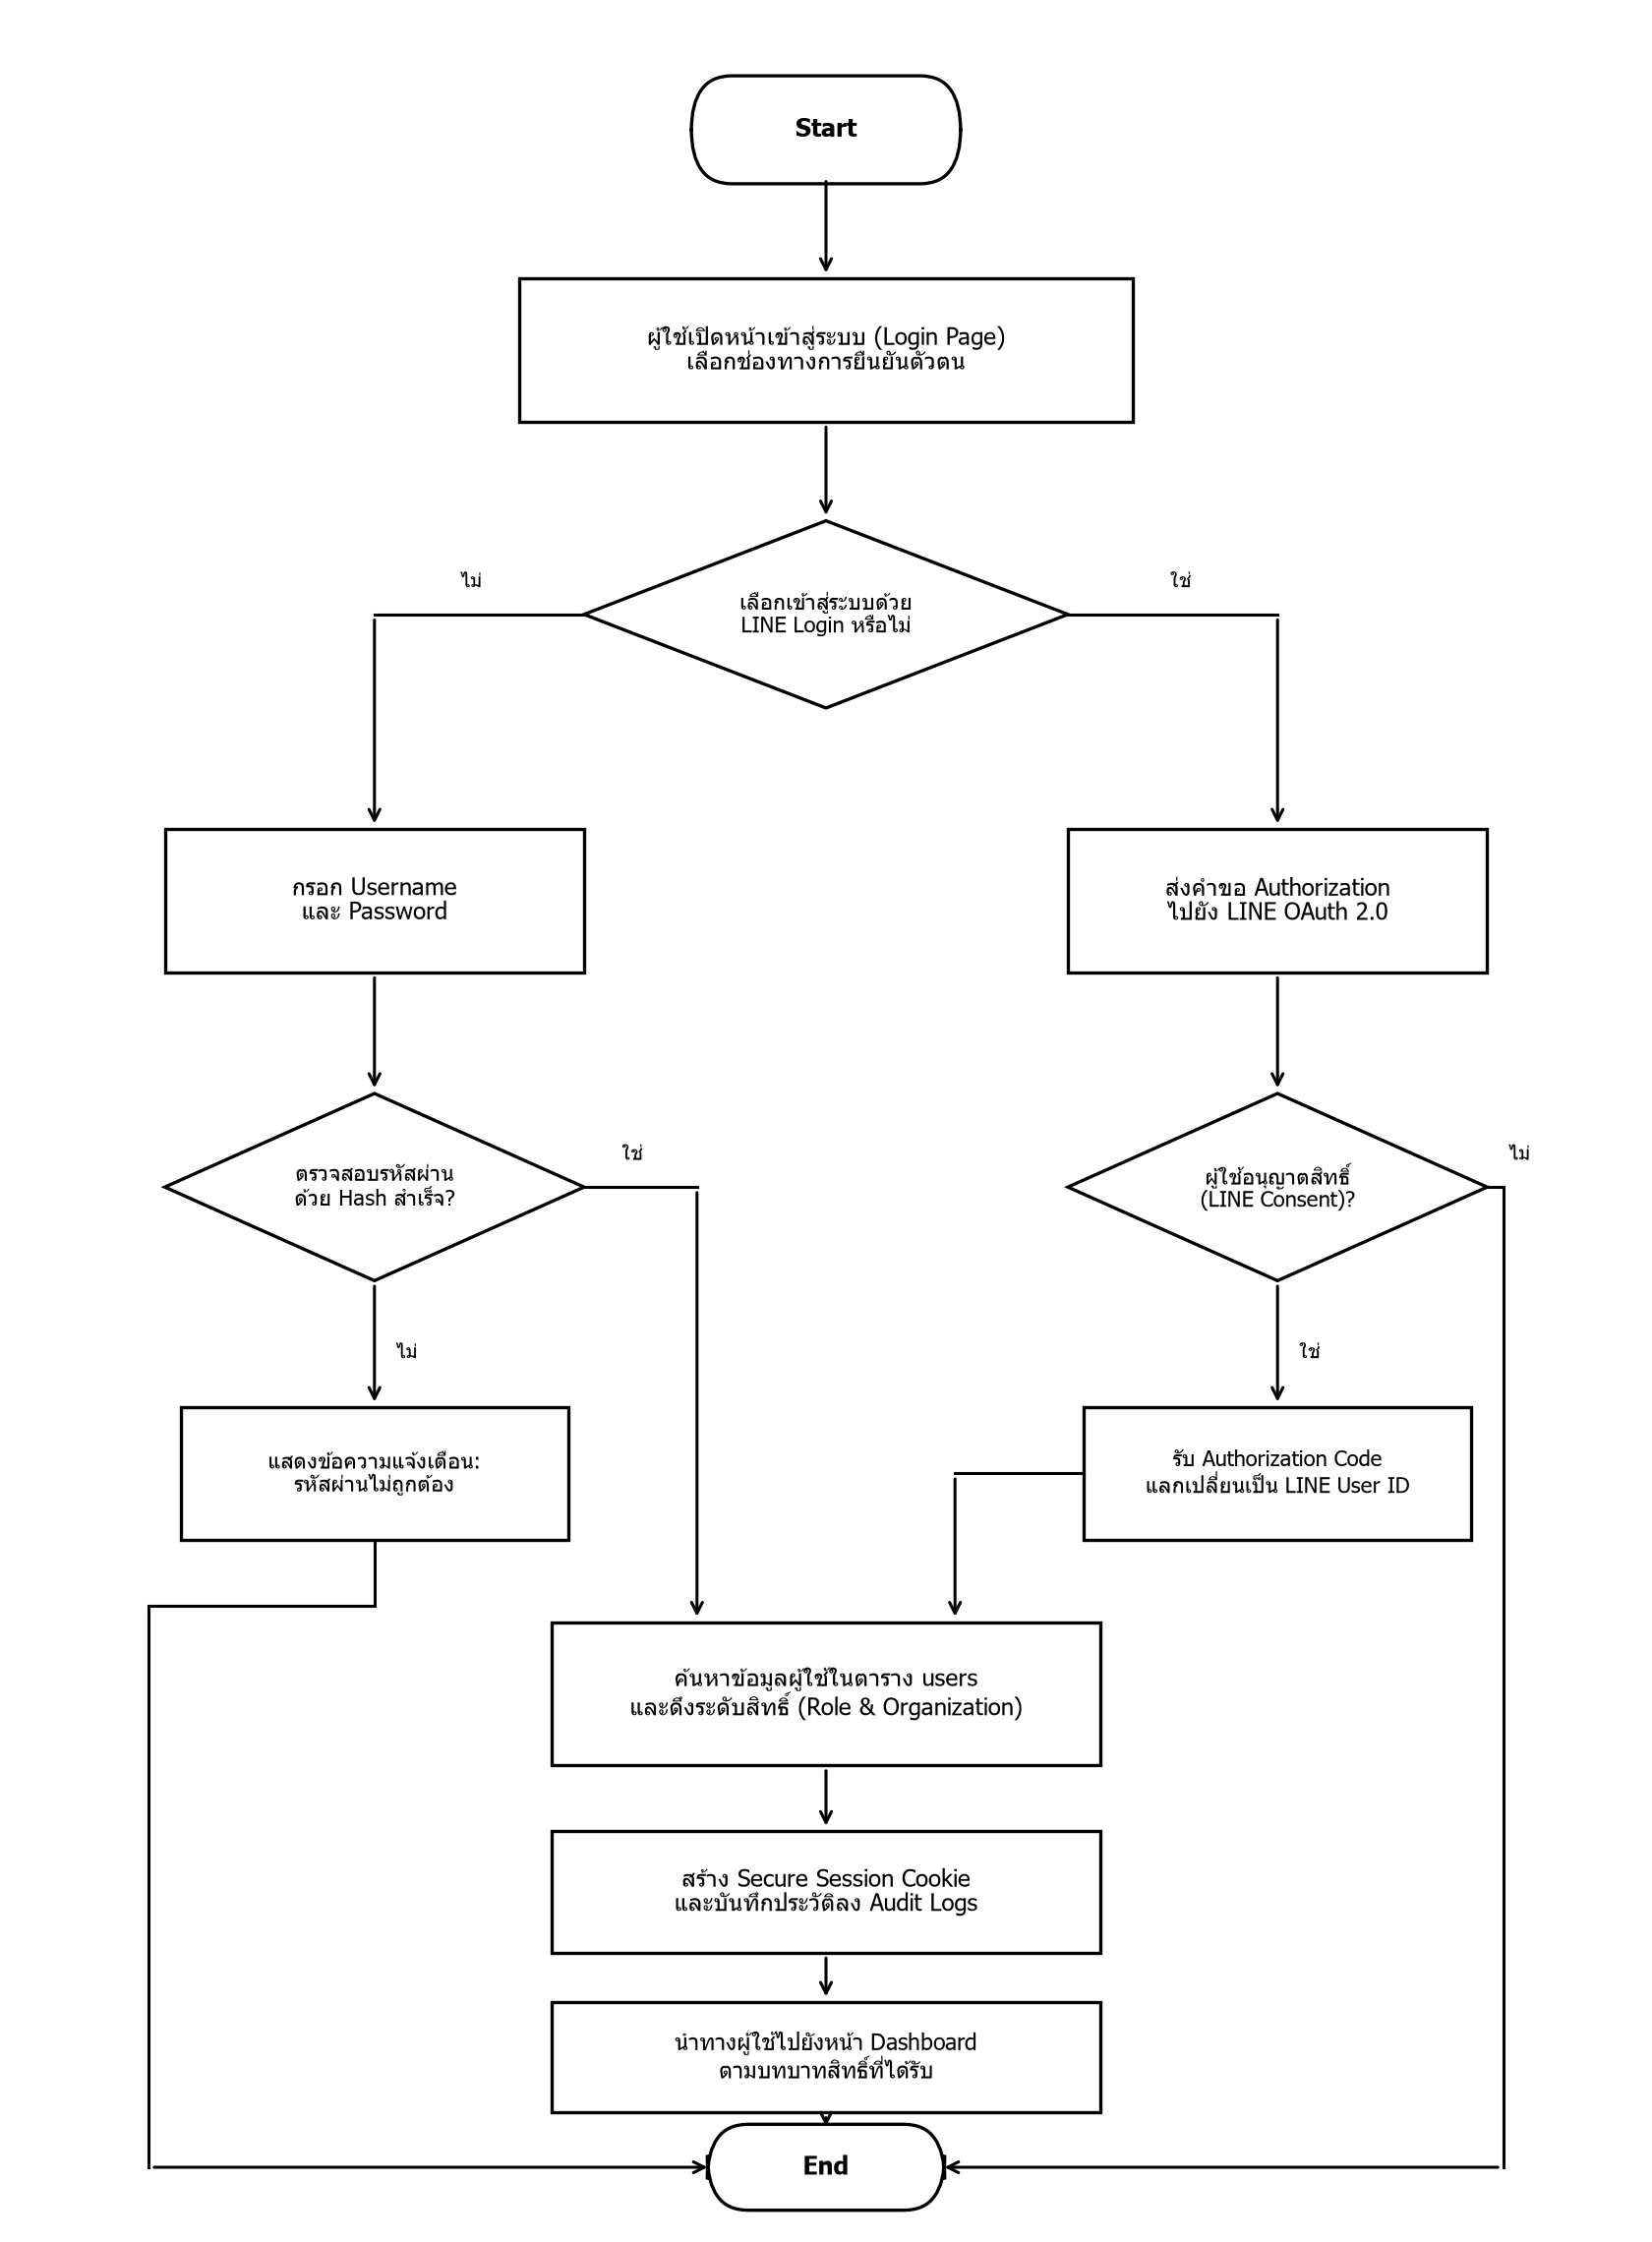
\includegraphics[height=0.46\textheight,keepaspectratio]{Image/fig3_3_flow_auth.png}
\caption{ผังงานขั้นตอนการเข้าสู่ระบบและการยืนยันตัวตน (Authentication Flowchart)}
\label{fig3:flow_auth}
\end{figure}

\subsection{ผังงานขั้นตอนการทำงานของระบบคลังความรู้ RAG (RAG Knowledge Retrieval Flowchart)}
\hspace*{1.3em}
แสดงขั้นตอนการแปลงคำถามภาษาธรรมชาติเป็นเวกเตอร์เอ็มเบดดิง การสืบค้นใน ChromaDB และตรวจสอบค่าคะแนนความคล้ายคลึง หากเกินเกณฑ์ 0.65 จะดึงท่อนบริบทส่งให้โมเดล Google Gemini 1.5 Flash สังเคราะห์คำตอบและจัดรูปแบบส่งกลับทาง LINE Flex Message ดังแสดงในภาพที่ 3-5:

\begin{figure}[htbp]
\centering
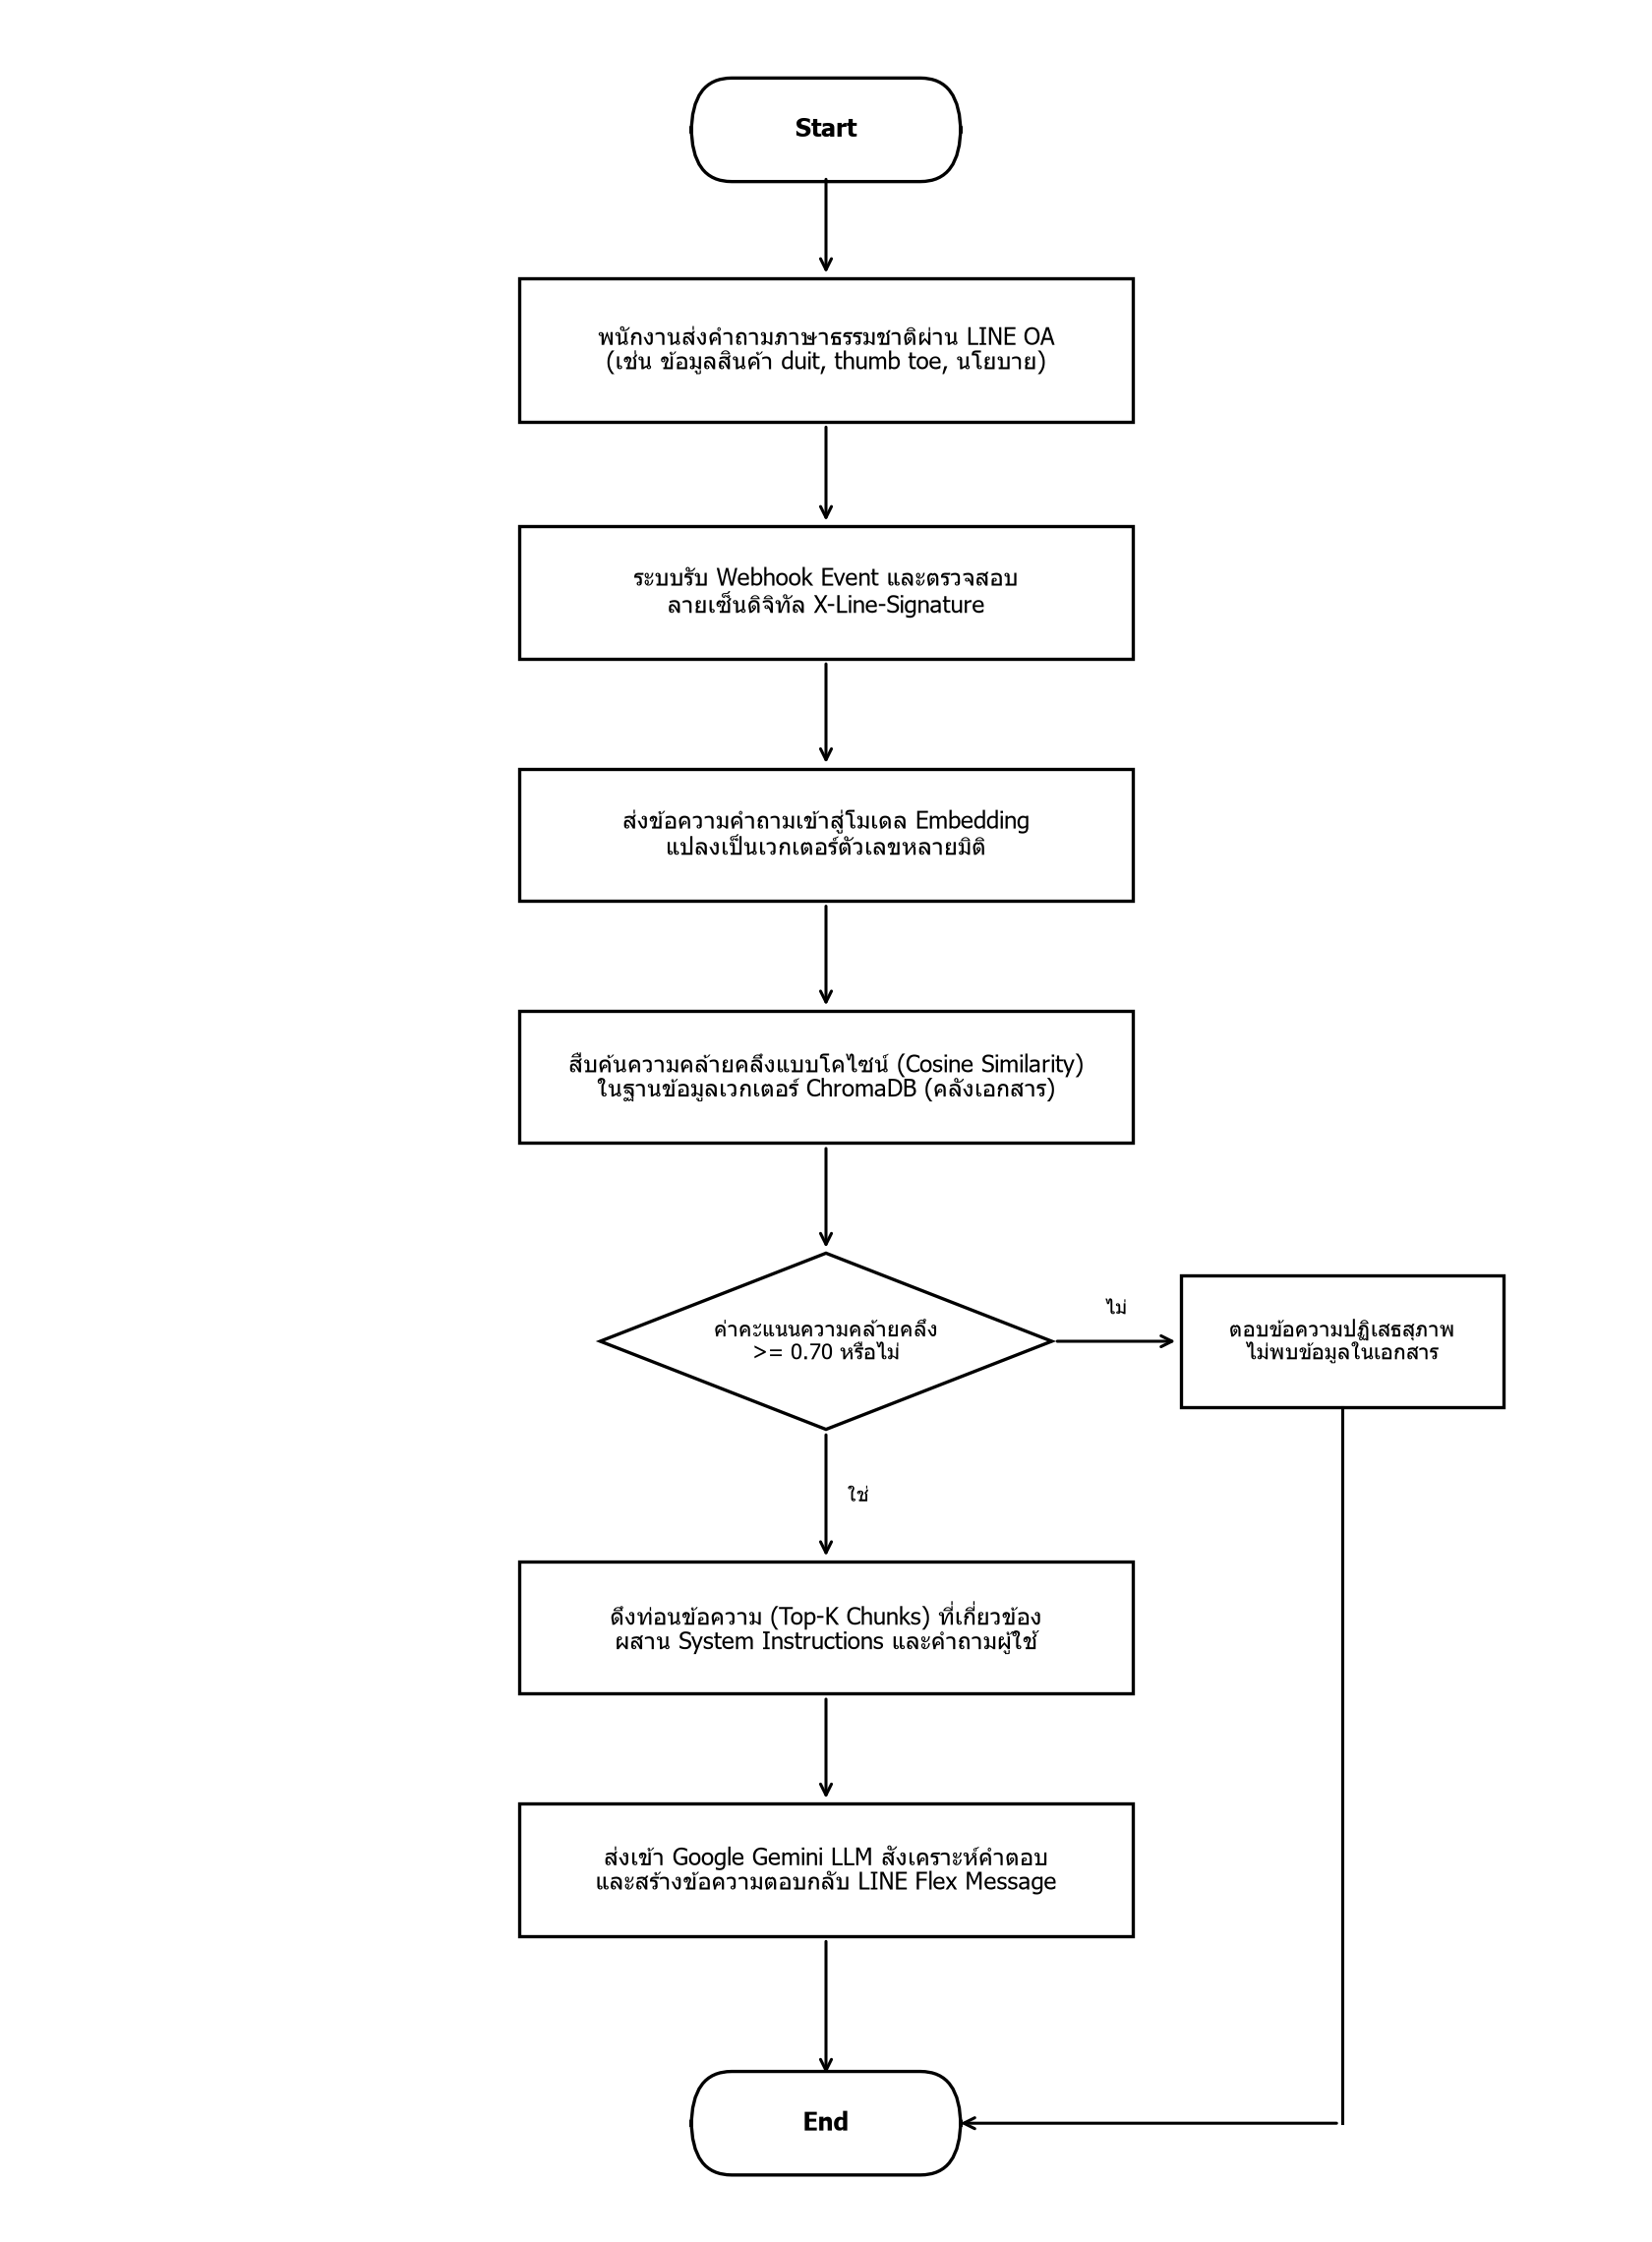
\includegraphics[height=0.46\textheight,keepaspectratio]{Image/fig3_6_flow_rag.png}
\caption{ผังงานขั้นตอนการทำงานของระบบคลังความรู้ RAG (RAG Knowledge Retrieval Flowchart)}
\label{fig3:flow_rag}
\end{figure}

\subsection{ผังงานขั้นตอนการสกัดข้อมูลสลิปและใบเสร็จด้วย OCR (OCR \& Bookkeeping Flowchart)}
\hspace*{1.3em}
แสดงขั้นตอนการรับภาพสลิปโอนเงิน การปรับปรุงคุณภาพภาพ (Grayscale, Threshold, Denoise, Deskew) และส่งให้ Google Cloud Vision API ร่วมกับ Regex สกัดฟิลด์สำคัญ จากนั้นจำแนกหมวดหมู่บัญชี บันทึกลง Google Sheets และสำรองไฟล์ขึ้น Google Drive ดังแสดงในภาพที่ 3-6:

\begin{figure}[htbp]
\centering
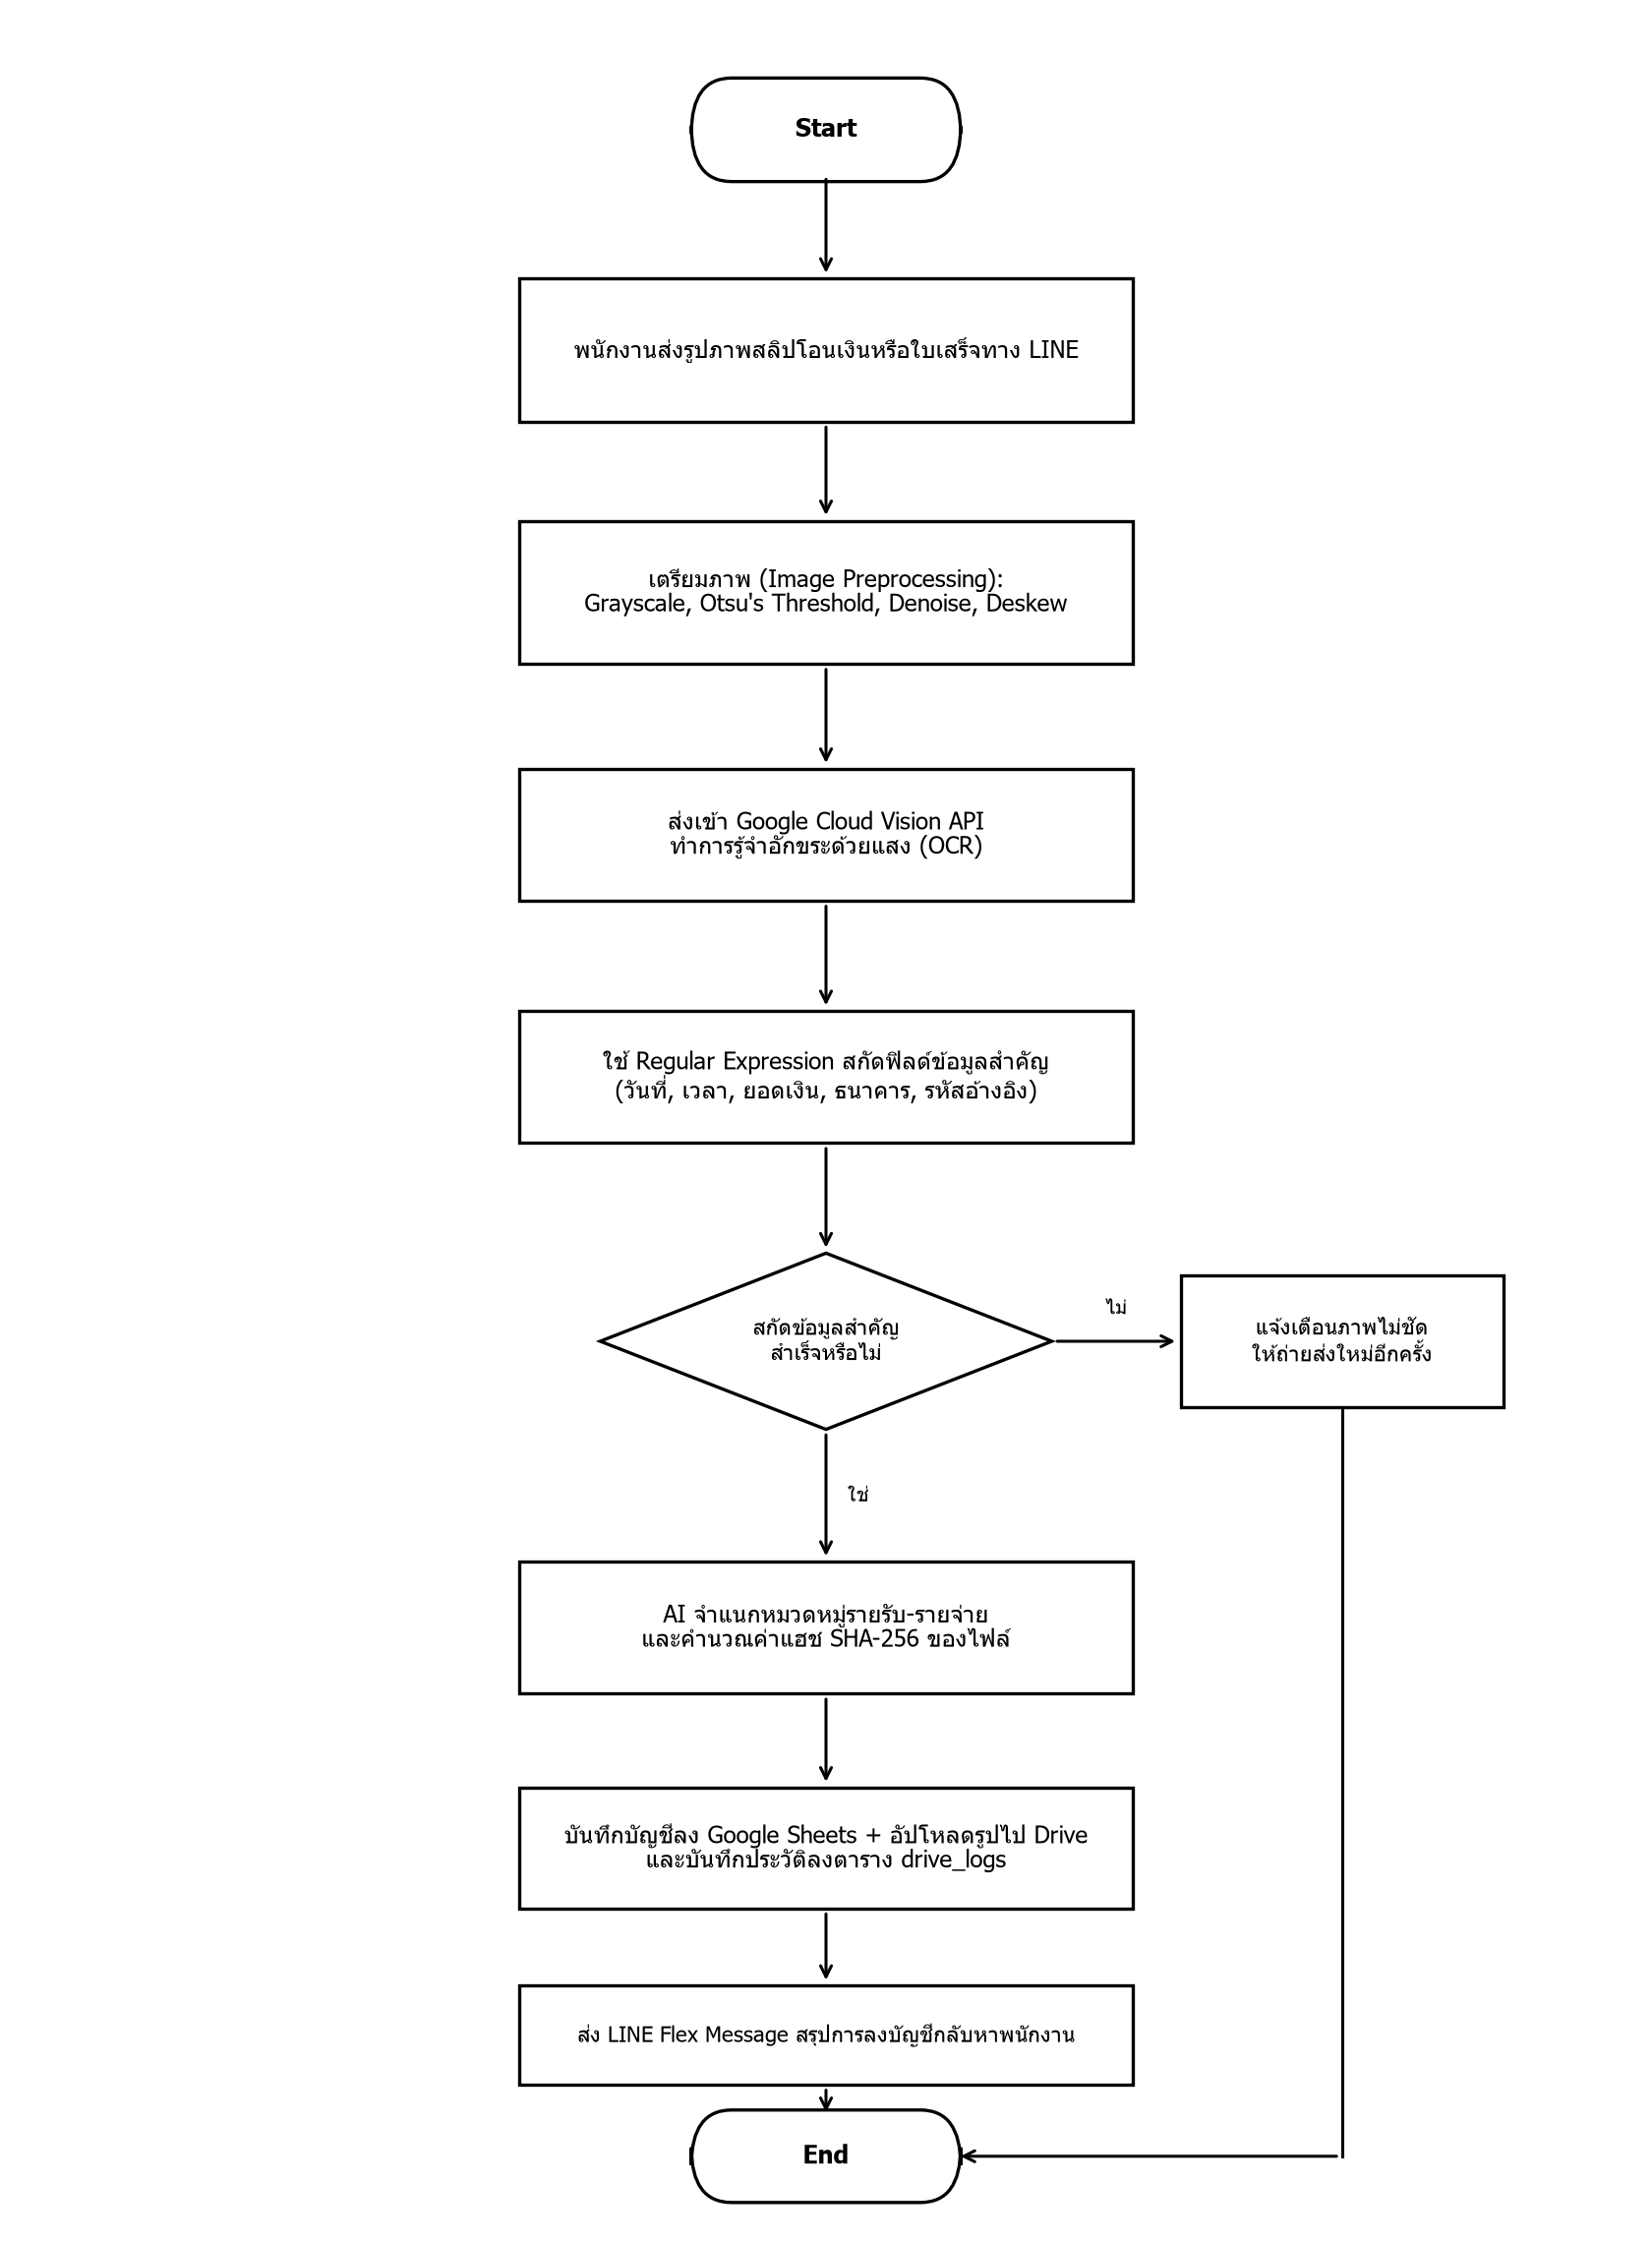
\includegraphics[height=0.46\textheight,keepaspectratio]{Image/fig3_7_flow_ocr.png}
\caption{ผังงานขั้นตอนการสกัดข้อมูลสลิปและใบเสร็จด้วย OCR และการลงบัญชีอัตโนมัติ}
\label{fig3:flow_ocr}
\end{figure}

\subsection{ผังงานขั้นตอนการยื่นคำขอลางานของพนักงาน (Leave Submission Flowchart)}
\hspace*{1.3em}
แสดงขั้นตอนเมื่อพนักงานเปิดเมนูยื่นใบลาจาก LINE Rich Menu ผ่านหน้าต่าง LIFF ระบุข้อมูลการลาและแนบเอกสารรับรอง ระบบจะตรวจสอบโควตาวันลาและบันทึกคำขอลงฐานข้อมูล พร้อมส่งการแจ้งเตือนไปยังหัวหน้างานทาง LINE Flex Message ดังแสดงในภาพที่ 3-7:

\begin{figure}[htbp]
\centering
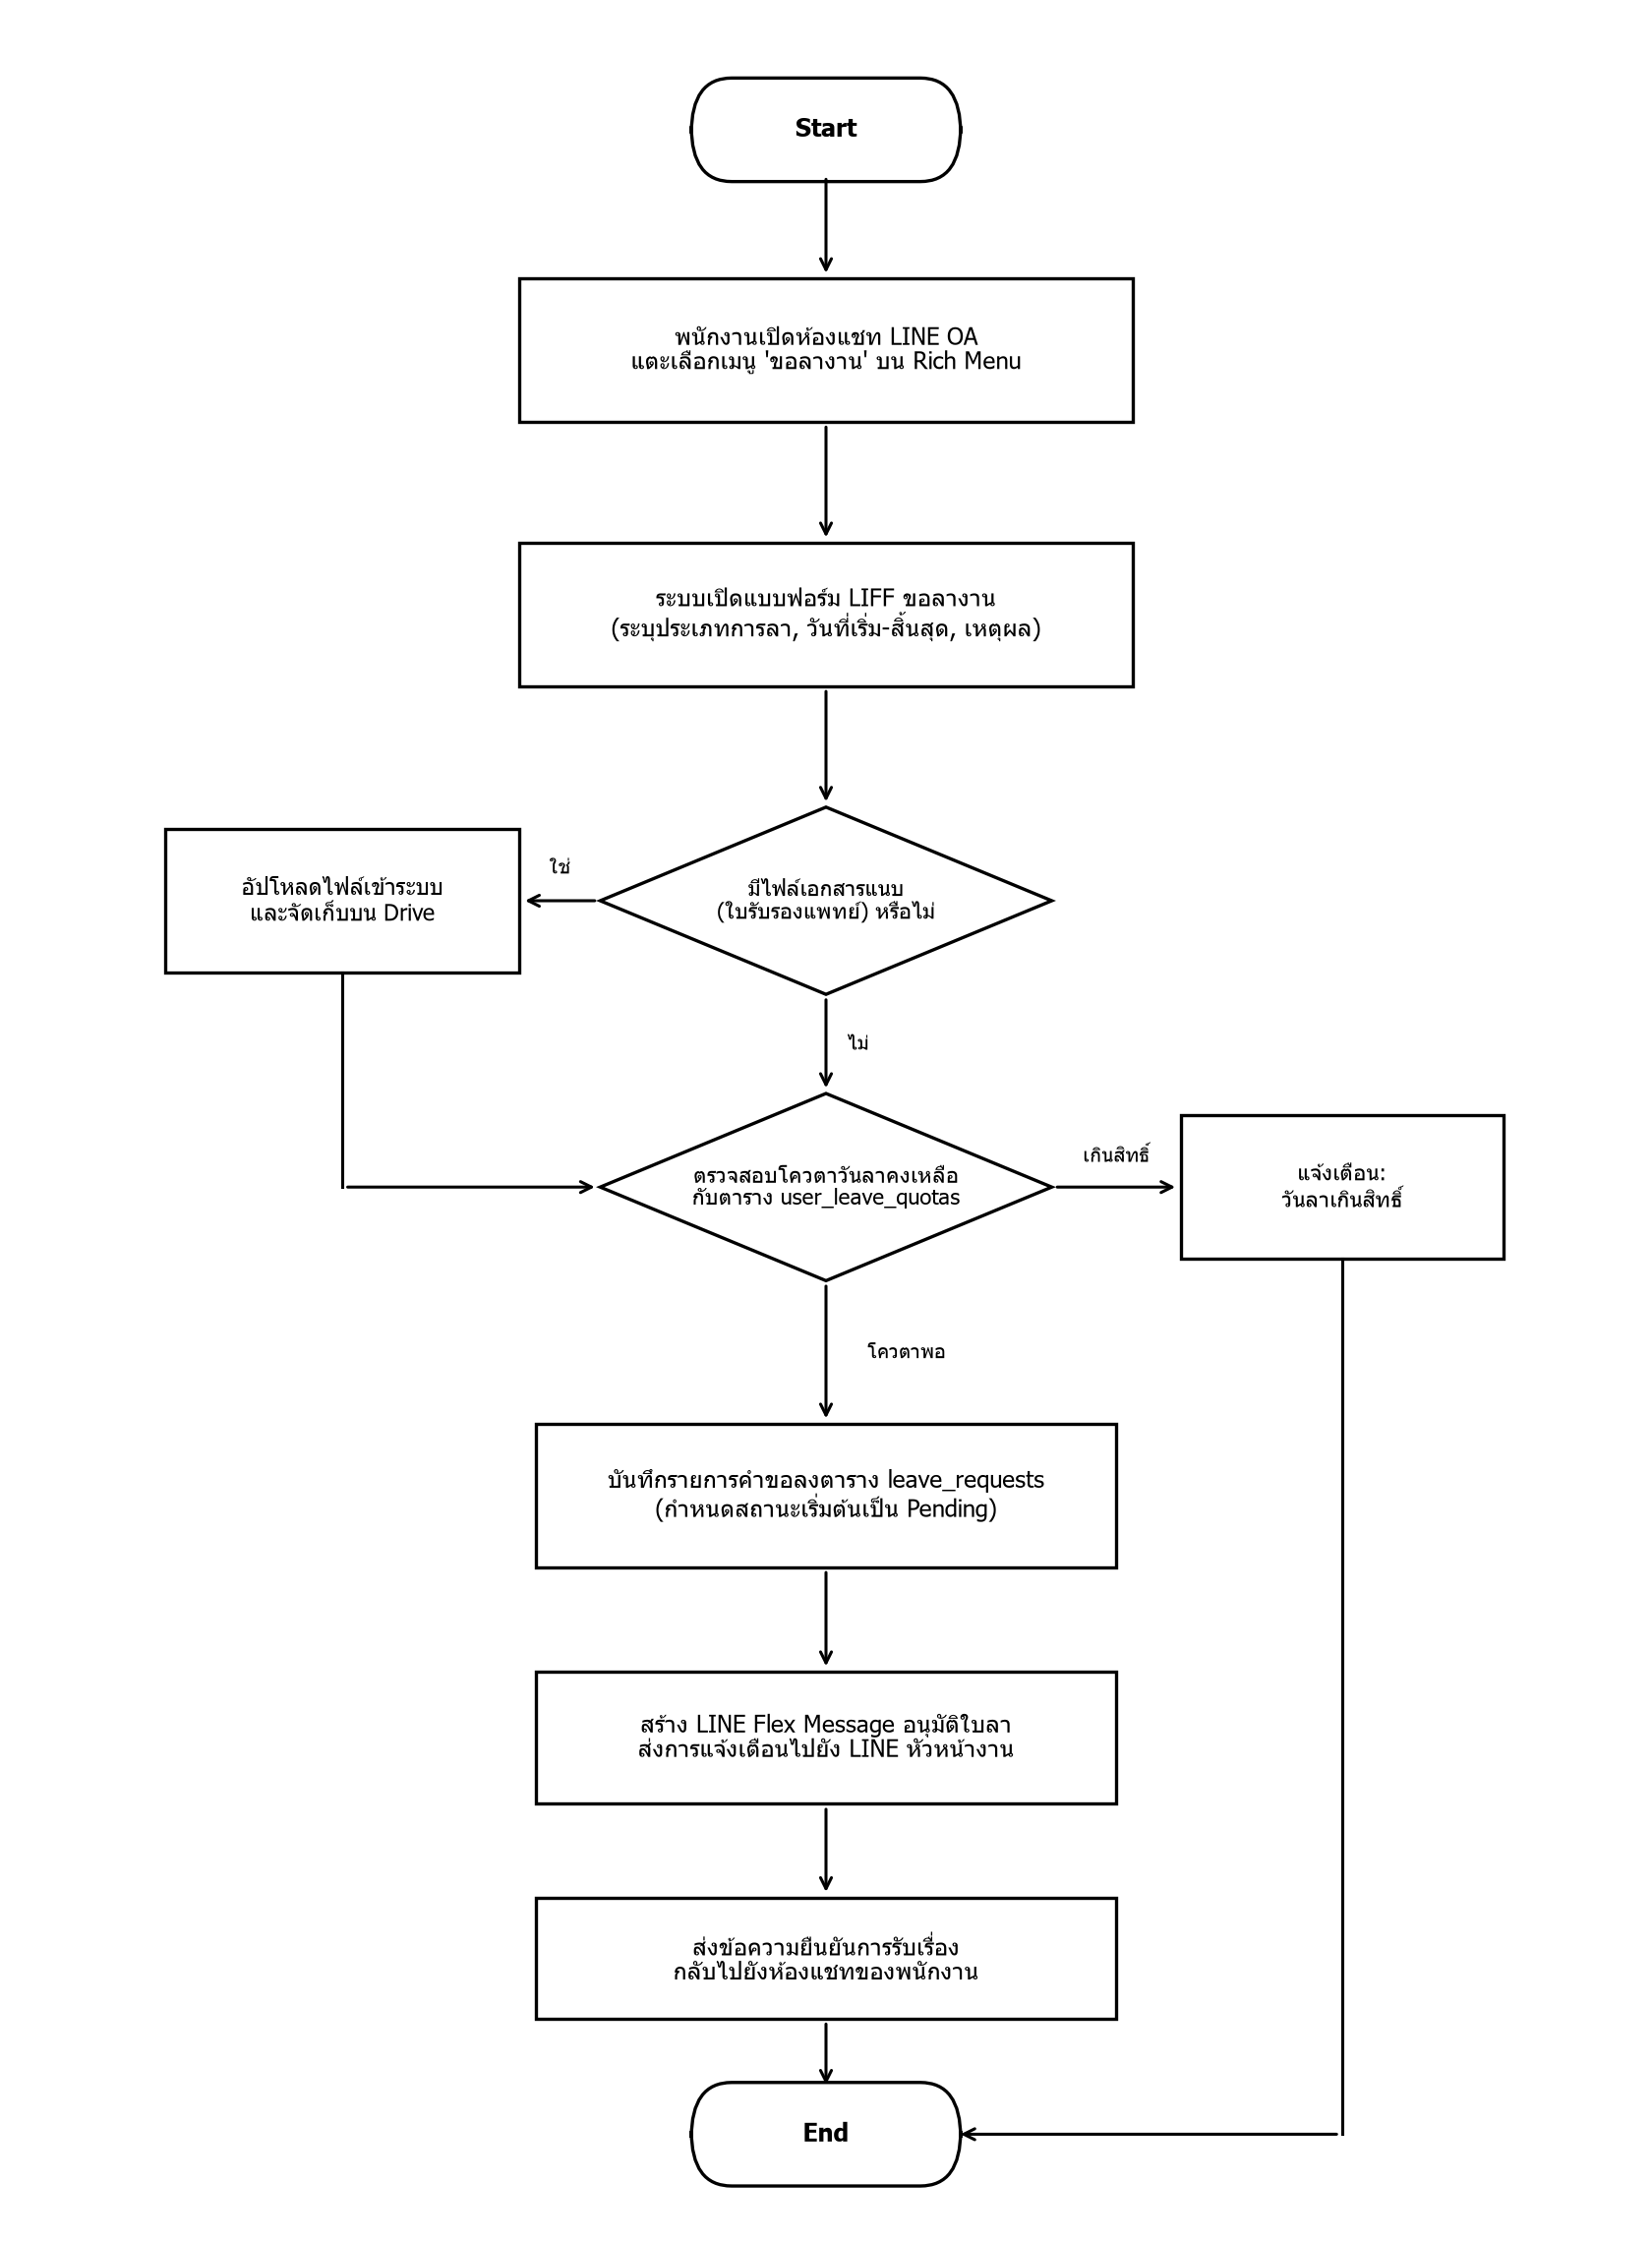
\includegraphics[height=0.46\textheight,keepaspectratio]{Image/fig3_5_flow_leave_request.png}
\caption{ผังงานขั้นตอนการยื่นคำขอลางานของพนักงานผ่าน LINE (Leave Submission Flowchart)}
\label{fig3:flow_leave_request}
\end{figure}

\subsection{ผังงานขั้นตอนการพิจารณาอนุมัติคำขอลางาน (Leave Approval Process Flowchart)}
\hspace*{1.3em}
แสดงเงื่อนไขและขั้นตอนการพิจารณาอนุมัติคำขอลางานของหัวหน้างาน เมื่อได้รับข้อความแจ้งเตือนทาง LINE Flex Message หากหัวหน้างานกดอนุมัติ ระบบจะตรวจสอบโควตาวันลา ปรับปรุงสถานะคำขอ หักลบโควตาวันลาในฐานข้อมูล และแจ้งผลกลับไปยังพนักงาน ดังแสดงในภาพที่ 3-8:

\begin{figure}[htbp]
\centering
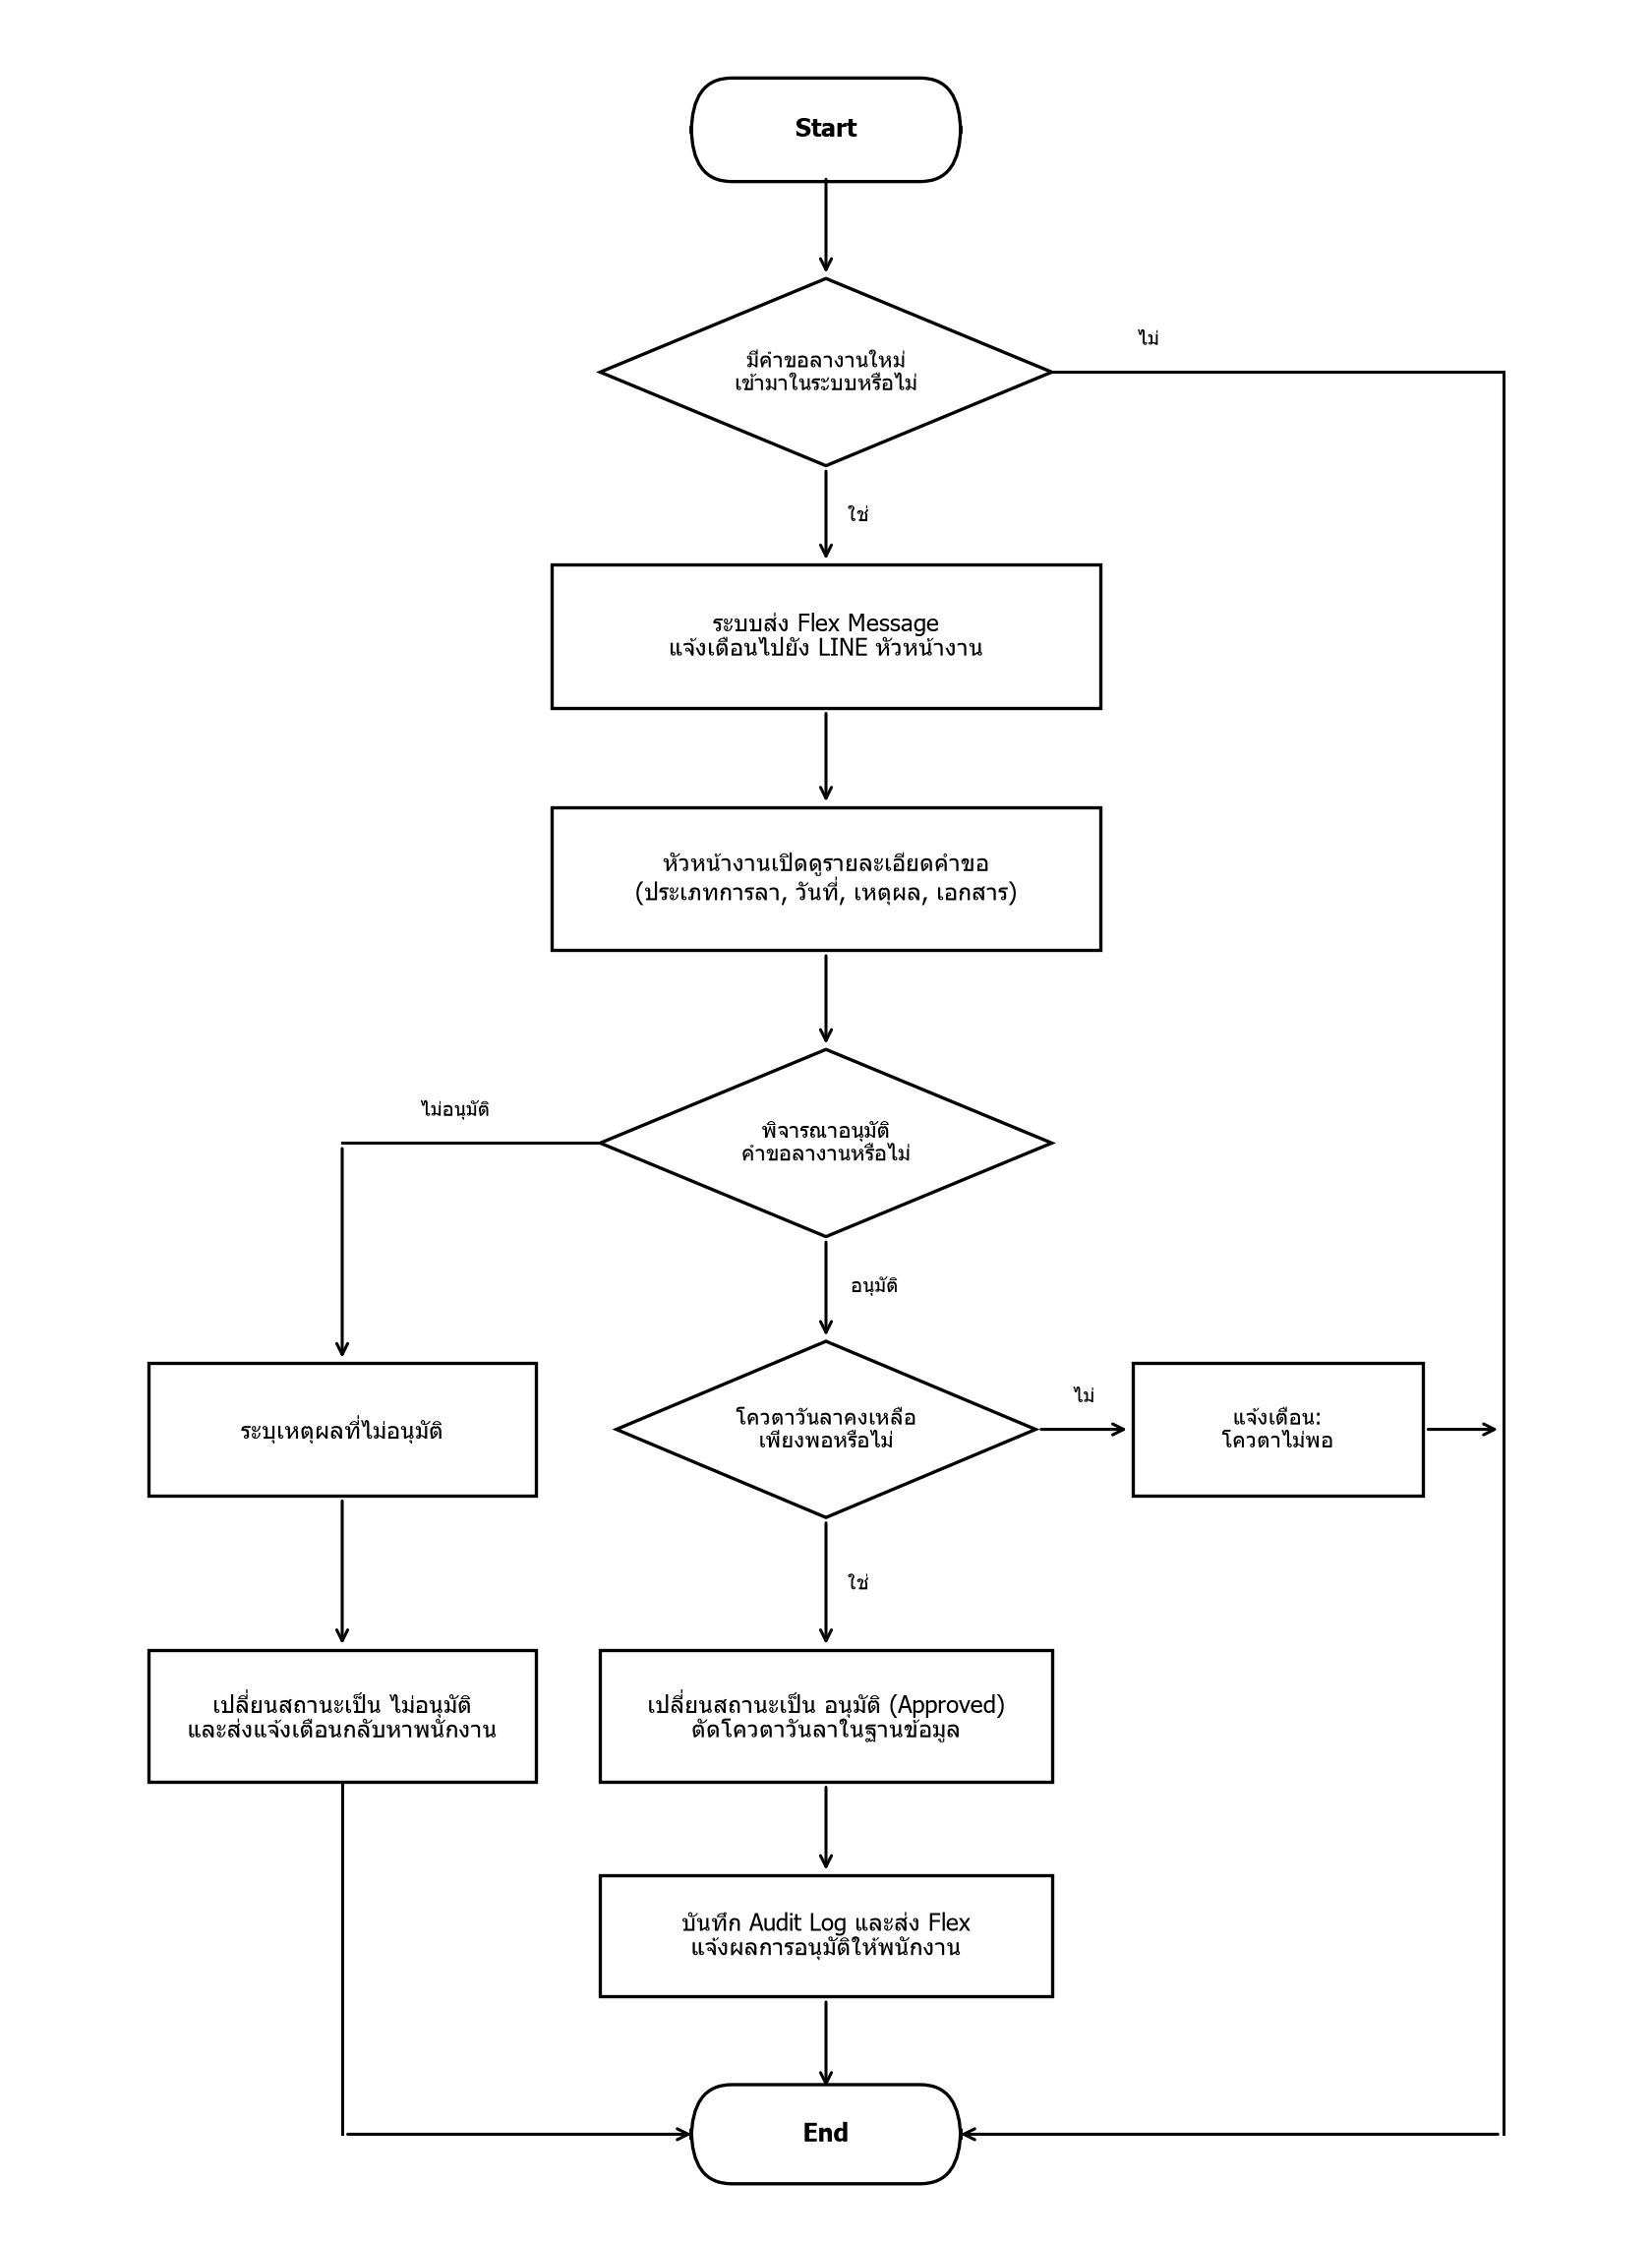
\includegraphics[height=0.46\textheight,keepaspectratio]{Image/fig3_4_flow_leave_approve.png}
\caption{ผังงานขั้นตอนการพิจารณาอนุมัติคำขอลางานของหัวหน้างาน (Leave Approval Flowchart)}
\label{fig3:flow_leave_approve}
\end{figure}

\clearpage
\section{การออกแบบฐานข้อมูล (Database Design)}
\hspace*{1.3em}
การออกแบบฐานข้อมูลเชิงสัมพันธ์ของระบบ OrgChat AI ถูกจัดโครงสร้างตามกฎการนอร์มัลไลเซชันระดับที่ 3 (3NF) เพื่อรักษาบูรณภาพของข้อมูล (Data Integrity) โดยมีแบบจำลองความสัมพันธ์ของข้อมูล (Entity Relationship Diagram: ER Diagram) แสดงดังภาพที่ 3-4:

\begin{figure}[htbp]
\centering
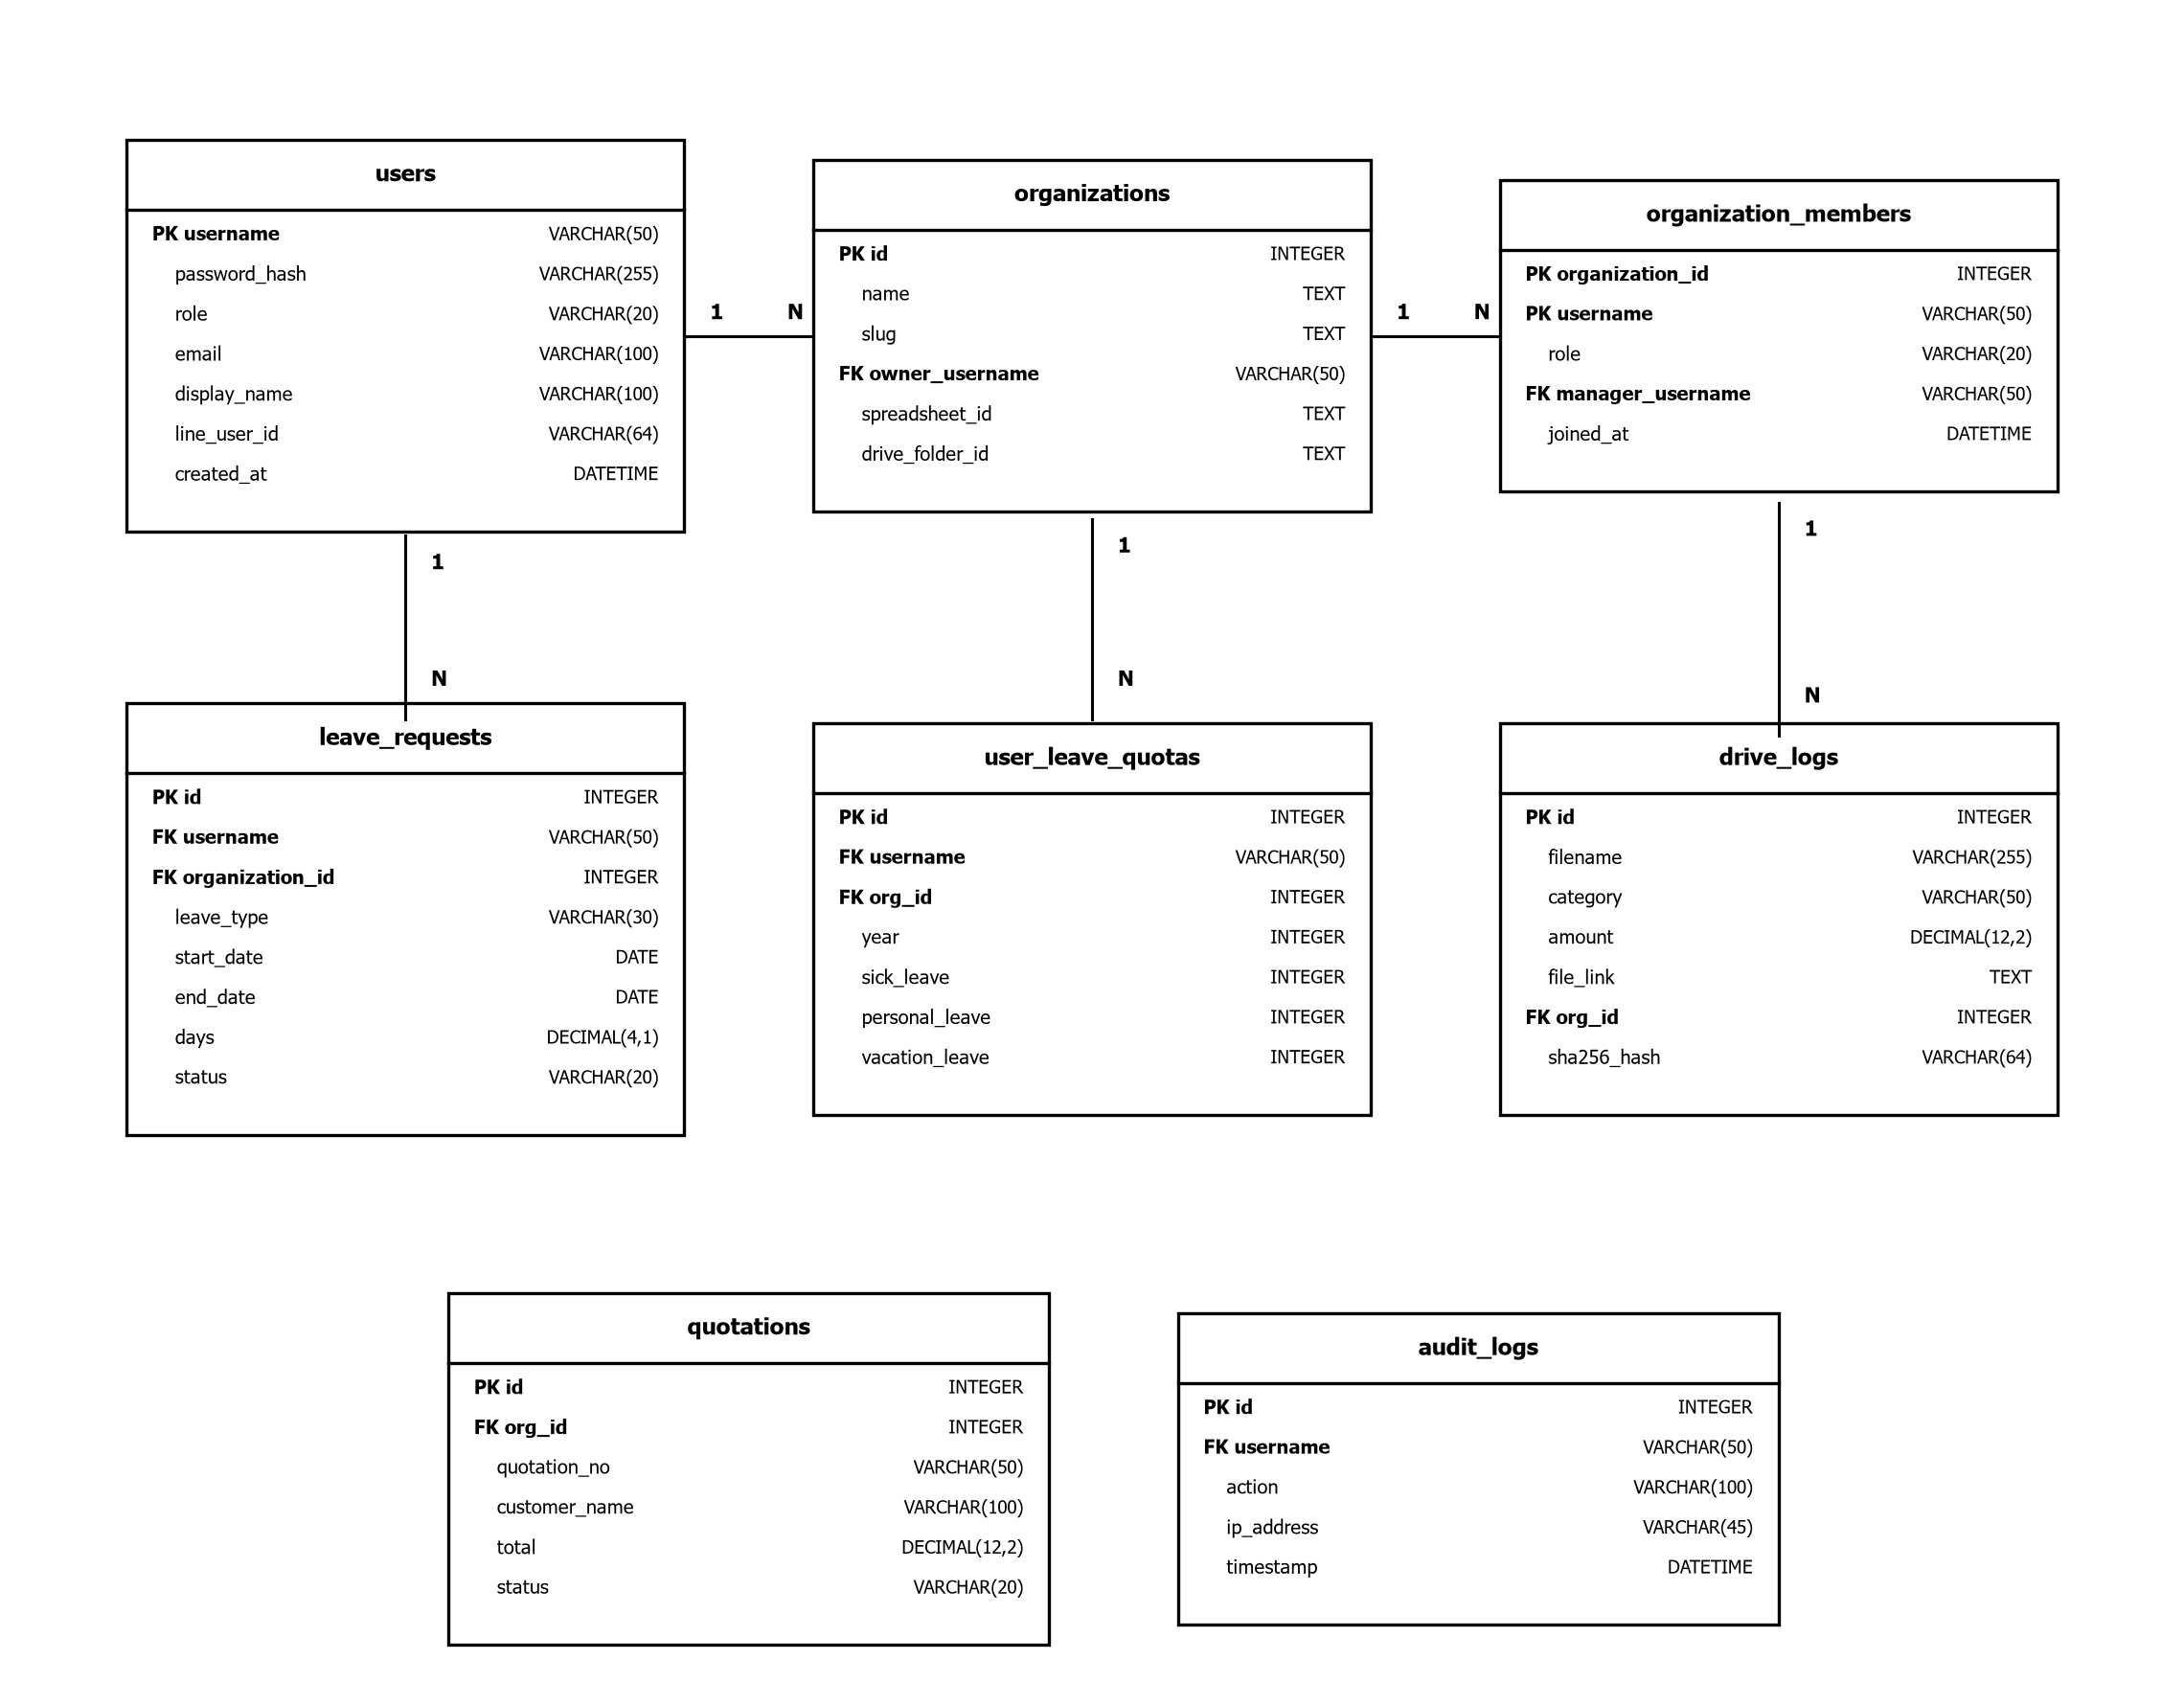
\includegraphics[width=0.95\textwidth]{Image/fig3_8_er_diagram.png}
\caption{Entity Relationship Diagram (ER Diagram) ของระบบ OrgChat AI}
\label{fig3:er_diagram}
\end{figure}

\subsection{รายการตารางข้อมูลในระบบ (Table List)}
\hspace*{1.3em}
ระบบฐานข้อมูลในภาคการศึกษาที่ 1/2569 ประกอบด้วยตารางข้อมูลหลักจำนวน 7 ตาราง ดังแสดงสรุปในตารางที่ 3-43:

\begin{table}[htbp]
\centering
\caption{รายชื่อตารางทั้งหมดในระบบฐานข้อมูล (Table List)}
\label{tab3:tablelist}
\begin{tabularx}{\textwidth}{| c | L | c | c |}
\hline
\textbf{ลำดับ} & \textbf{ชื่อตารางข้อมูล (Table Name)} & \textbf{ชื่อเอนทิตีภาษาไทย} & \textbf{คีย์หลัก (Primary Key)} \\ \hline
1 & users & ข้อมูลบัญชีผู้ใช้งานระบบ & id \\ \hline
2 & organizations & ข้อมูลบริษัทและองค์กร & id \\ \hline
3 & documents & ข้อมูลเอกสารในคลังความรู้ & id \\ \hline
4 & document\_chunks & ข้อมูลท่อนข้อความเอกสาร & id \\ \hline
5 & line\_sessions & ข้อมูลเซสชันการสนทนา LINE & id \\ \hline
6 & drive\_logs & บันทึกประวัติไฟล์บน Google Drive & id \\ \hline
7 & audit\_logs & บันทึกประวัติความปลอดภัยและการทำงาน & id \\ \hline
\end{tabularx}
\end{table}

\subsection{โครงสร้างตารางข้อมูลอย่างละเอียด (Table Layouts)}
\hspace*{1.3em}
รายละเอียดโครงสร้างของแต่ละตารางในฐานข้อมูล แสดงดังตารางที่ 3-44 ถึงตารางที่ 3-50:

\begin{table}[htbp]
\centering
\caption{โครงสร้างตารางข้อมูล users (ผู้ใช้งานระบบ)}
\label{tab3:tb_users}
\begin{tabularx}{\textwidth}{| c | c | c | c | c | L |}
\hline
\textbf{Attribute} & \textbf{Type} & \textbf{Length} & \textbf{Key} & \textbf{Null} & \textbf{Description} \\ \hline
id & INTEGER & - & PK & No & รหัสประจำตัวผู้ใช้ (Auto Increment) \\ \hline
username & VARCHAR & 50 & Unique & No & ชื่อบัญชีผู้ใช้งาน \\ \hline
password\_hash & VARCHAR & 255 & - & No & รหัสผ่านที่เข้ารหัสแฮชด้วย BCrypt \\ \hline
role & VARCHAR & 20 & - & No & ระดับบทบาท (admin, manager, user) \\ \hline
email & VARCHAR & 100 & - & Yes & อีเมลติดต่อของผู้ใช้งาน \\ \hline
display\_name & VARCHAR & 100 & - & Yes & ชื่อ-นามสกุลที่ใช้แสดงผล \\ \hline
line\_user\_id & VARCHAR & 64 & - & Yes & รหัสประจำตัวบนแพลตฟอร์ม LINE \\ \hline
org\_id & INTEGER & - & FK & Yes & รหัสองค์กรที่สังกัด (อ้างอิง organizations.id) \\ \hline
created\_at & DATETIME & - & - & No & วันและเวลาที่สร้างบัญชี \\ \hline
\end{tabularx}
\end{table}

\begin{table}[htbp]
\centering
\caption{โครงสร้างตารางข้อมูล organizations (ข้อมูลองค์กร)}
\label{tab3:tb_orgs}
\begin{tabularx}{\textwidth}{| c | c | c | c | c | L |}
\hline
\textbf{Attribute} & \textbf{Type} & \textbf{Length} & \textbf{Key} & \textbf{Null} & \textbf{Description} \\ \hline
id & INTEGER & - & PK & No & รหัสประจำตัวองค์กร (Auto Increment) \\ \hline
org\_name & VARCHAR & 100 & - & No & ชื่อบริษัท (บจก. ฮาร์ทวอมมิ่ง) \\ \hline
domain & VARCHAR & 100 & - & Yes & โดเมนเนมอีเมลขององค์กร \\ \hline
line\_channel\_token & TEXT & - & - & Yes & Channel Access Token ของ LINE OA \\ \hline
created\_at & DATETIME & - & - & No & วันและเวลาที่ลงทะเบียนองค์กร \\ \hline
status & VARCHAR & 20 & - & No & สถานะการใช้งาน (Active, Suspended) \\ \hline
\end{tabularx}
\end{table}

\begin{table}[htbp]
\centering
\caption{โครงสร้างตารางข้อมูล documents (เอกสารคลังความรู้)}
\label{tab3:tb_docs}
\begin{tabularx}{\textwidth}{| c | c | c | c | c | L |}
\hline
\textbf{Attribute} & \textbf{Type} & \textbf{Length} & \textbf{Key} & \textbf{Null} & \textbf{Description} \\ \hline
id & INTEGER & - & PK & No & รหัสประจำตัวเอกสาร (Auto Increment) \\ \hline
file\_name & VARCHAR & 255 & - & No & ชื่อไฟล์เอกสารต้นฉบับ \\ \hline
file\_path & VARCHAR & 500 & - & No & ตำแหน่งจัดเก็บไฟล์บนเซิร์ฟเวอร์ \\ \hline
file\_hash & VARCHAR & 64 & - & No & ค่าแฮช SHA-256 สำหรับตรวจไฟล์ซ้ำ \\ \hline
file\_size & INTEGER & - & - & No & ขนาดของไฟล์เอกสาร (ไบต์) \\ \hline
file\_type & VARCHAR & 20 & - & No & นามสกุลไฟล์ (pdf, docx, txt, xlsx) \\ \hline
org\_id & INTEGER & - & FK & No & รหัสองค์กรเจ้าของเอกสาร \\ \hline
uploaded\_by & INTEGER & - & FK & No & รหัสผู้ใช้อัปโหลด (อ้างอิง users.id) \\ \hline
status & VARCHAR & 20 & - & No & สถานะเอกสาร (PROCESSING, READY, ERROR) \\ \hline
created\_at & DATETIME & - & - & No & วันเวลาที่อัปโหลดเอกสาร \\ \hline
\end{tabularx}
\end{table}

\begin{table}[htbp]
\centering
\caption{โครงสร้างตารางข้อมูล document\_chunks (ท่อนข้อความเอกสาร)}
\label{tab3:tb_chunks}
\begin{tabularx}{\textwidth}{| c | c | c | c | c | L |}
\hline
\textbf{Attribute} & \textbf{Type} & \textbf{Length} & \textbf{Key} & \textbf{Null} & \textbf{Description} \\ \hline
id & INTEGER & - & PK & No & รหัสประจำตัวท่อนข้อความ (Auto Increment) \\ \hline
doc\_id & INTEGER & - & FK & No & รหัสเอกสารต้นทาง (อ้างอิง documents.id) \\ \hline
chunk\_index & INTEGER & - & - & No & ลำดับของท่อนข้อความในเอกสาร \\ \hline
chunk\_text & TEXT & - & - & No & เนื้อหาข้อความของท่อนข้อมูล \\ \hline
page\_number & INTEGER & - & - & Yes & เลขหน้าที่พบท่อนข้อความในเอกสาร \\ \hline
vector\_id & VARCHAR & 64 & - & Yes & รหัสอ้างอิงเวกเตอร์ใน ChromaDB \\ \hline
created\_at & DATETIME & - & - & No & วันเวลาที่สร้างท่อนข้อความ \\ \hline
\end{tabularx}
\end{table}

\begin{table}[htbp]
\centering
\caption{โครงสร้างตารางข้อมูล line\_sessions (เซสชันการสนทนา LINE)}
\label{tab3:tb_sessions}
\begin{tabularx}{\textwidth}{| c | c | c | c | c | L |}
\hline
\textbf{Attribute} & \textbf{Type} & \textbf{Length} & \textbf{Key} & \textbf{Null} & \textbf{Description} \\ \hline
id & INTEGER & - & PK & No & รหัสบันทึกเซสชัน (Auto Increment) \\ \hline
line\_user\_id & VARCHAR & 64 & - & No & รหัสผู้ใช้งานบน LINE \\ \hline
last\_message & TEXT & - & - & Yes & ข้อความล่าสุดที่ส่งเข้ามา \\ \hline
last\_reply & TEXT & - & - & Yes & ข้อความตอบกลับล่าสุดจากระบบ \\ \hline
context\_state & VARCHAR & 50 & - & Yes & สถานะบริบทการสนทนาปัจจุบัน \\ \hline
updated\_at & DATETIME & - & - & No & วันเวลาที่มีการโต้ตอบล่าสุด \\ \hline
\end{tabularx}
\end{table}

\begin{table}[htbp]
\centering
\caption{โครงสร้างตารางข้อมูล drive\_logs (ประวัติไฟล์บน Google Drive)}
\label{tab3:tb_drive}
\begin{tabularx}{\textwidth}{| c | c | c | c | c | L |}
\hline
\textbf{Attribute} & \textbf{Type} & \textbf{Length} & \textbf{Key} & \textbf{Null} & \textbf{Description} \\ \hline
id & INTEGER & - & PK & No & รหัสบันทึกประวัติไฟล์ (Auto Increment) \\ \hline
file\_name & VARCHAR & 255 & - & No & ชื่อไฟล์ที่อัปโหลดขึ้น Drive \\ \hline
drive\_file\_id & VARCHAR & 100 & - & No & รหัสไฟล์จาก Google Drive API \\ \hline
drive\_url & VARCHAR & 500 & - & Yes & ลิงก์ URL สำหรับเข้าถึงไฟล์ \\ \hline
folder\_path & VARCHAR & 255 & - & Yes & โฟลเดอร์ปลายทางบน Drive \\ \hline
org\_id & INTEGER & - & FK & No & รหัสองค์กรเจ้าของไฟล์ \\ \hline
uploaded\_by & VARCHAR & 64 & - & Yes & ผู้ส่งไฟล์ (line\_user\_id หรือ username) \\ \hline
created\_at & DATETIME & - & - & No & วันเวลาที่จัดเก็บไฟล์ \\ \hline
\end{tabularx}
\end{table}

\begin{table}[htbp]
\centering
\caption{โครงสร้างตารางข้อมูล audit\_logs (บันทึกกิจกรรมความปลอดภัย)}
\label{tab3:tb_audit}
\begin{tabularx}{\textwidth}{| c | c | c | c | c | L |}
\hline
\textbf{Attribute} & \textbf{Type} & \textbf{Length} & \textbf{Key} & \textbf{Null} & \textbf{Description} \\ \hline
id & INTEGER & - & PK & No & รหัสบันทึกกิจกรรม (Auto Increment) \\ \hline
user\_id & VARCHAR & 50 & - & No & ผู้ใช้ที่ทำกิจกรรมในระบบ \\ \hline
action & VARCHAR & 100 & - & No & ประเภทกิจกรรม (LOGIN, RAG\_QUERY, UPLOAD) \\ \hline
details & TEXT & - & - & Yes & รายละเอียดหรือพารามิเตอร์ของกิจกรรม \\ \hline
ip\_address & VARCHAR & 45 & - & Yes & หมายเลข IP Address ของเครื่องผู้ใช้ \\ \hline
created\_at & DATETIME & - & - & No & วันเวลาที่เกิดกิจกรรมตามเวลาเซิร์ฟเวอร์ \\ \hline
\end{tabularx}
\end{table}

\section{การออกแบบส่วนต่อประสานผู้ใช้ (User Interface Design)}
\hspace*{1.3em}
การออกแบบส่วนต่อประสานผู้ใช้ (UI/UX Design) มุ่งเน้นการใช้งานที่ง่ายและตอบโจทย์พนักงาน บริษัท ฮาร์ทวอมมิ่ง จำกัด โดยออกแบบเส้นทางการทำงาน (Screen Flow) เชื่อมโยงระหว่างแอปพลิเคชัน LINE OA กับเว็บแอปพลิเคชันระบบบริหารจัดการ ดังแสดงในภาพที่ 3-5:

\begin{figure}[htbp]
\centering
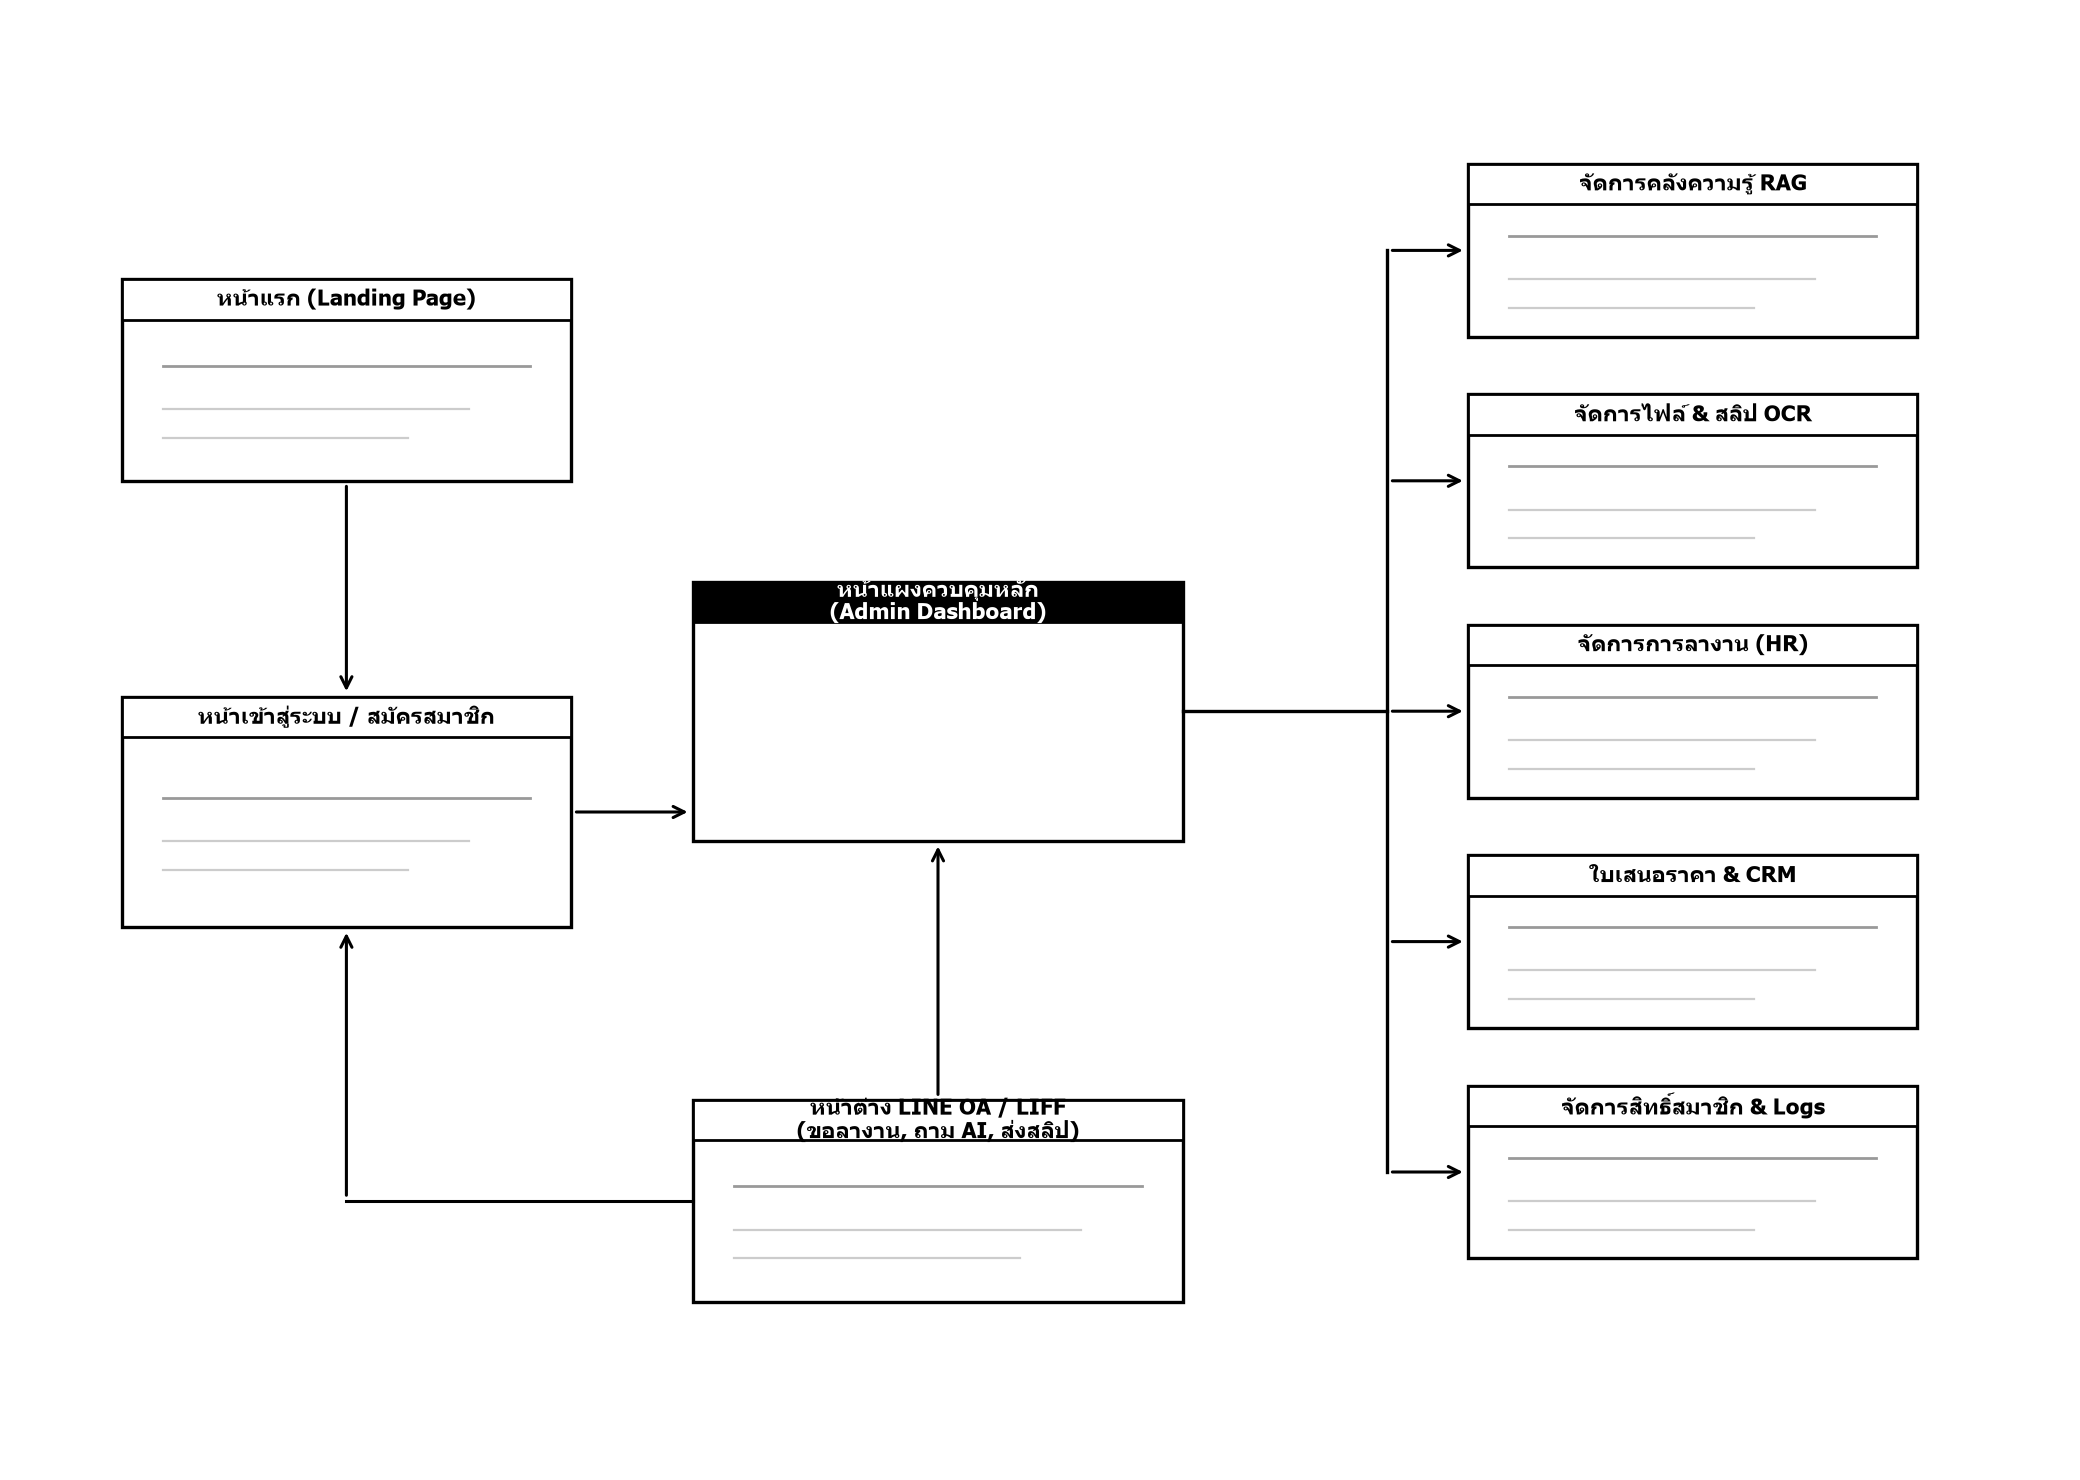
\includegraphics[width=0.95\textwidth]{Image/fig3_9_screen_flow.png}
\caption{แผนผังลำดับการทำงานของหน้าจอ (Screen Flow Diagram)}
\label{fig3:screen_flow}
\end{figure}

\subsection{การออกแบบหน้าจอหลักของระบบ (Main Screen Layouts)}
\hspace*{1.3em}
การออกแบบหน้าจอของระบบในภาคการศึกษาที่ 1/2569 ประกอบด้วย 3 ส่วนสำคัญ ได้แก่:
\begin{enumerate}[leftmargin=3.5em]
\item \textbf{หน้าจอเข้าสู่ระบบและยืนยันตัวตน (Login Screen):} ออกแบบฟอร์มการเข้าสู่ระบบแบบ Responsive รองรับการกรอก Username/Password สำหรับผู้ดูแลระบบ และปุ่มลงชื่อเข้าใช้ด้วย Google Sign-In (OAuth 2.0) รวมถึงระบบสแกน QR Code สำหรับพนักงาน เพื่อความสะดวกรวดเร็ว
\item \textbf{หน้าจอจัดการคลังความรู้ (Knowledge Base Management Screen):} หน้าจอเว็บสำหรับผู้ดูแลระบบ แสดงรายการเอกสารที่อัปโหลด แถบแสดงสถานะการแปลงเวกเตอร์ (Processing / Ready) ขนาดไฟล์ จำนวนท่อนข้อความ (Chunks) และปุ่มสำหรับอัปโหลดไฟล์เอกสารใหม่
\item \textbf{หน้าต่างการสนทนา LINE Official Account (LINE OA Chat Screen):} หน้าต่างสนทนาบนแอปพลิเคชัน LINE ออกแบบ Rich Menu ด้านล่างสำหรับการสอบถามข้อมูลด่วน และการแสดงผลคำตอบด้วย LINE Flex Message ที่มีสีสันสวยงาม อ่านง่าย พร้อมปุ่มลิงก์ไปยังข้อมูลสินค้าเพิ่มเติม
\end{enumerate}

    %*************************************
% บทที่ 4
%*************************************
\chapterTitle{4}{ผลการดำเนินงาน}
\vspace{0.2in}
\hspace*{1.3em}
ในบทนี้จะนำเสนอผลการพัฒนาระบบปัญญาประดิษฐ์แชทบอทสำหรับองค์กร กรณีศึกษา บริษัท ฮาร์ทวอมมิ่ง จำกัด ตามขอบเขตการดำเนินงานในภาคการศึกษาที่ 1/2569 ซึ่งมุ่งเน้นการพัฒนาระบบส่วนโครงสร้างพื้นฐาน ได้แก่ ระบบยืนยันตัวตนและจัดการบัญชีผู้ใช้งาน, ระบบคลังความรู้อัจฉริยะ (Retrieval-Augmented Generation: RAG), ระบบแชทบอท LINE Official Account ผ่าน LINE Messaging API, และระบบจัดการเอกสารเชื่อมโยง Google Drive จากนั้นนำเสนอผลการทดสอบการทำงานของระบบเบื้องต้น (Functional Black-Box Testing) และสรุปสถานะการดำเนินงานเปรียบเทียบกับขอบเขตของโครงงานที่ได้รับอนุมัติในแบบเสนอ ทก.01

\section{ภาพรวมของระบบที่พัฒนาแล้วเสร็จ}
\hspace*{1.3em}
ระบบที่พัฒนาขึ้นในภาคการศึกษาที่ 1/2569 เป็นระบบเว็บแอปพลิเคชันร่วมกับแชทบอทบนแพลตฟอร์ม LINE โดยฝั่งเซิร์ฟเวอร์พัฒนาด้วยภาษา Python ร่วมกับเว็บเฟรมเวิร์ก Flask ใช้ฐานข้อมูล SQLite ในการจัดเก็บข้อมูลเชิงสัมพันธ์ ใช้ ChromaDB ร่วมกับ FastEmbed ในการจัดเก็บและสืบค้นเวกเตอร์เอ็มเบดดิง และเชื่อมต่อกับ Google Gemini 1.5 Flash API ในการสังเคราะห์คำตอบภาษาธรรมชาติ ระบบแบ่งออกเป็น 4 ส่วนหลักตามที่ได้กำหนดไว้ในขอบเขตเทอม 1 ดังแสดงในตารางที่ 4-1:

\begin{table}[htbp]
\centering
\caption{ส่วนประกอบหลักของระบบและหน้าที่การทำงานในภาคการศึกษาที่ 1/2569}
\label{tab4:modules}
\begin{tabularx}{\textwidth}{| L | L | c |}
\hline
\textbf{ส่วนของระบบ} & \textbf{หน้าที่หลักการทำงาน} & \textbf{กลุ่มผู้ใช้งาน} \\ \hline
1. ระบบยืนยันตัวตนและจัดการบัญชีผู้ใช้ & สมัครสมาชิก เข้าสู่ระบบด้วย Email/Password, Google Sign-In (OAuth 2.0) และการผูกบัญชี LINE จัดการข้อมูลโปรไฟล์ และควบคุมเซสชัน & ผู้ดูแลระบบ, พนักงาน \\ \hline
2. ระบบคลังความรู้อัจฉริยะ (RAG System) & อัปโหลดเอกสารคู่มือสินค้าและระเบียบปฏิบัติ (PDF, TXT, CSV) สกัดข้อความ ตัดแบ่งท่อนข้อมูล แปลงเวกเตอร์เอ็มเบดดิง และบันทึกลง ChromaDB & ผู้ดูแลระบบ (Admin) \\ \hline
3. ระบบแชทบอท LINE Official Account & รับข้อความคำถามภาษาธรรมชาติผ่าน LINE Messaging API Webhook ค้นหาบริบทในคลังความรู้ สังเคราะห์คำตอบด้วย Gemini และตอบกลับด้วย LINE Flex Message & พนักงานทั่วไป \\ \hline
4. ระบบจัดการเอกสารเชื่อมโยง Google Drive & จัดเก็บและสำรองไฟล์เอกสารขึ้นสู่ Google Drive แยกโฟลเดอร์ตามปีและเดือนอัตโนมัติ พร้อมบันทึกประวัติการจัดเก็บไฟล์ & ผู้ดูแลระบบ, พนักงาน \\ \hline
\end{tabularx}
\end{table}

\section{ผลการพัฒนาระบบยืนยันตัวตนและการเข้าสู่ระบบ}
\hspace*{1.3em}
ผู้ใช้งานสามารถเข้าสู่ระบบเว็บแอปพลิเคชัน OrgChat AI เพื่อเข้าถึงการจัดการคลังความรู้และข้อมูลส่วนตัว โดยระบบรองรับการเข้าสู่ระบบ 2 รูปแบบ ได้แก่: 1) การเข้าสู่ระบบด้วยชื่อผู้ใช้หรืออีเมลและรหัสผ่าน สำหรับผู้ดูแลระบบ ซึ่งรหัสผ่านจะถูกเข้ารหัสแฮชด้วยอัลกอริทึม BCrypt และ 2) การลงชื่อเข้าใช้ด้วย Google Sign-In (OAuth 2.0) และระบบสแกน QR Code สำหรับพนักงานทั่วไป ซึ่งช่วยอำนวยความสะดวกให้พนักงานสามารถเข้าสู่ระบบได้ทันทีโดยไม่ต้องจดจำรหัสผ่านใหม่ ดังแสดงในภาพที่ 4-1:

\begin{figure}[htbp]
\centering
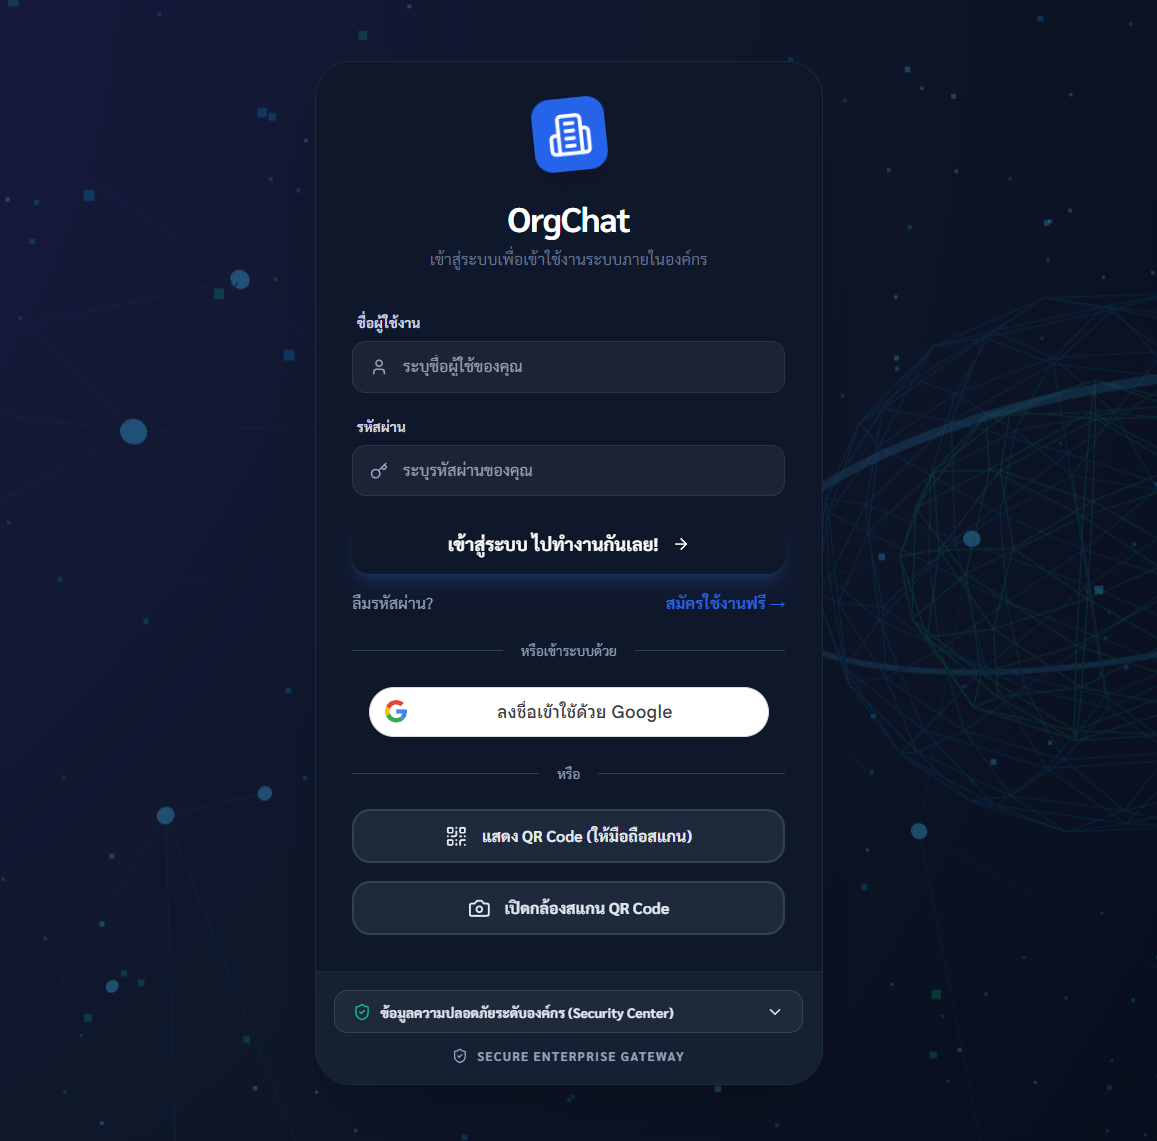
\includegraphics[width=0.95\textwidth]{Image/fig4_1_login.png}
\caption{หน้าจอเข้าสู่ระบบและสมัครสมาชิกผ่านเว็บแอปพลิเคชัน}
\label{fig4:login}
\end{figure}

\hspace*{1.3em}
จากภาพที่ 4-1 เมื่อผู้ใช้งานเข้าสู่ระบบสำเร็จ ระบบจะสร้าง JWT Session Token จัดเก็บไว้ในเบราว์เซอร์อย่างปลอดภัย และทำการตรวจสอบระดับสิทธิ์ (Role-Based Access Control) เพื่ออนุญาตให้เข้าถึงหน้าจอการทำงานที่สอดคล้องกับบทบาทของผู้ใช้ โดยผู้ดูแลระบบ (Admin) จะสามารถเข้าถึงหน้าจัดการคลังความรู้และการตั้งค่าระบบ ขณะที่พนักงานทั่วไปจะเข้าถึงหน้าโปรไฟล์และการตั้งค่าบัญชีส่วนตัว

\section{ผลการพัฒนาระบบคลังความรู้อัจฉริยะ (RAG System)}
\hspace*{1.3em}
ระบบคลังความรู้อัจฉริยะ (Retrieval-Augmented Generation) ได้รับการพัฒนาขึ้นเพื่อแก้ปัญหาข้อมูลสินค้าและเอกสารองค์กรกระจัดกระจาย โดยผู้ดูแลระบบสามารถอัปโหลดไฟล์เอกสารจริงของ บริษัท ฮาร์ทวอมมิ่ง จำกัด เช่น คู่มือการใช้งานสินค้าแบรนด์ duit (เครื่องให้อาหารสัตว์เลี้ยงอัตโนมัติ, น้ำพุแมว), รายละเอียดสินค้าแบรนด์ thumb toe (ถุงเท้าพิลาทิส), ข้อมูลสินค้า by.tuneteller, และระเบียบปฏิบัติต่าง ๆ เข้าสู่ระบบผ่านหน้าเว็บแอปพลิเคชัน ดังแสดงในภาพที่ 4-2:

\begin{figure}[htbp]
\centering
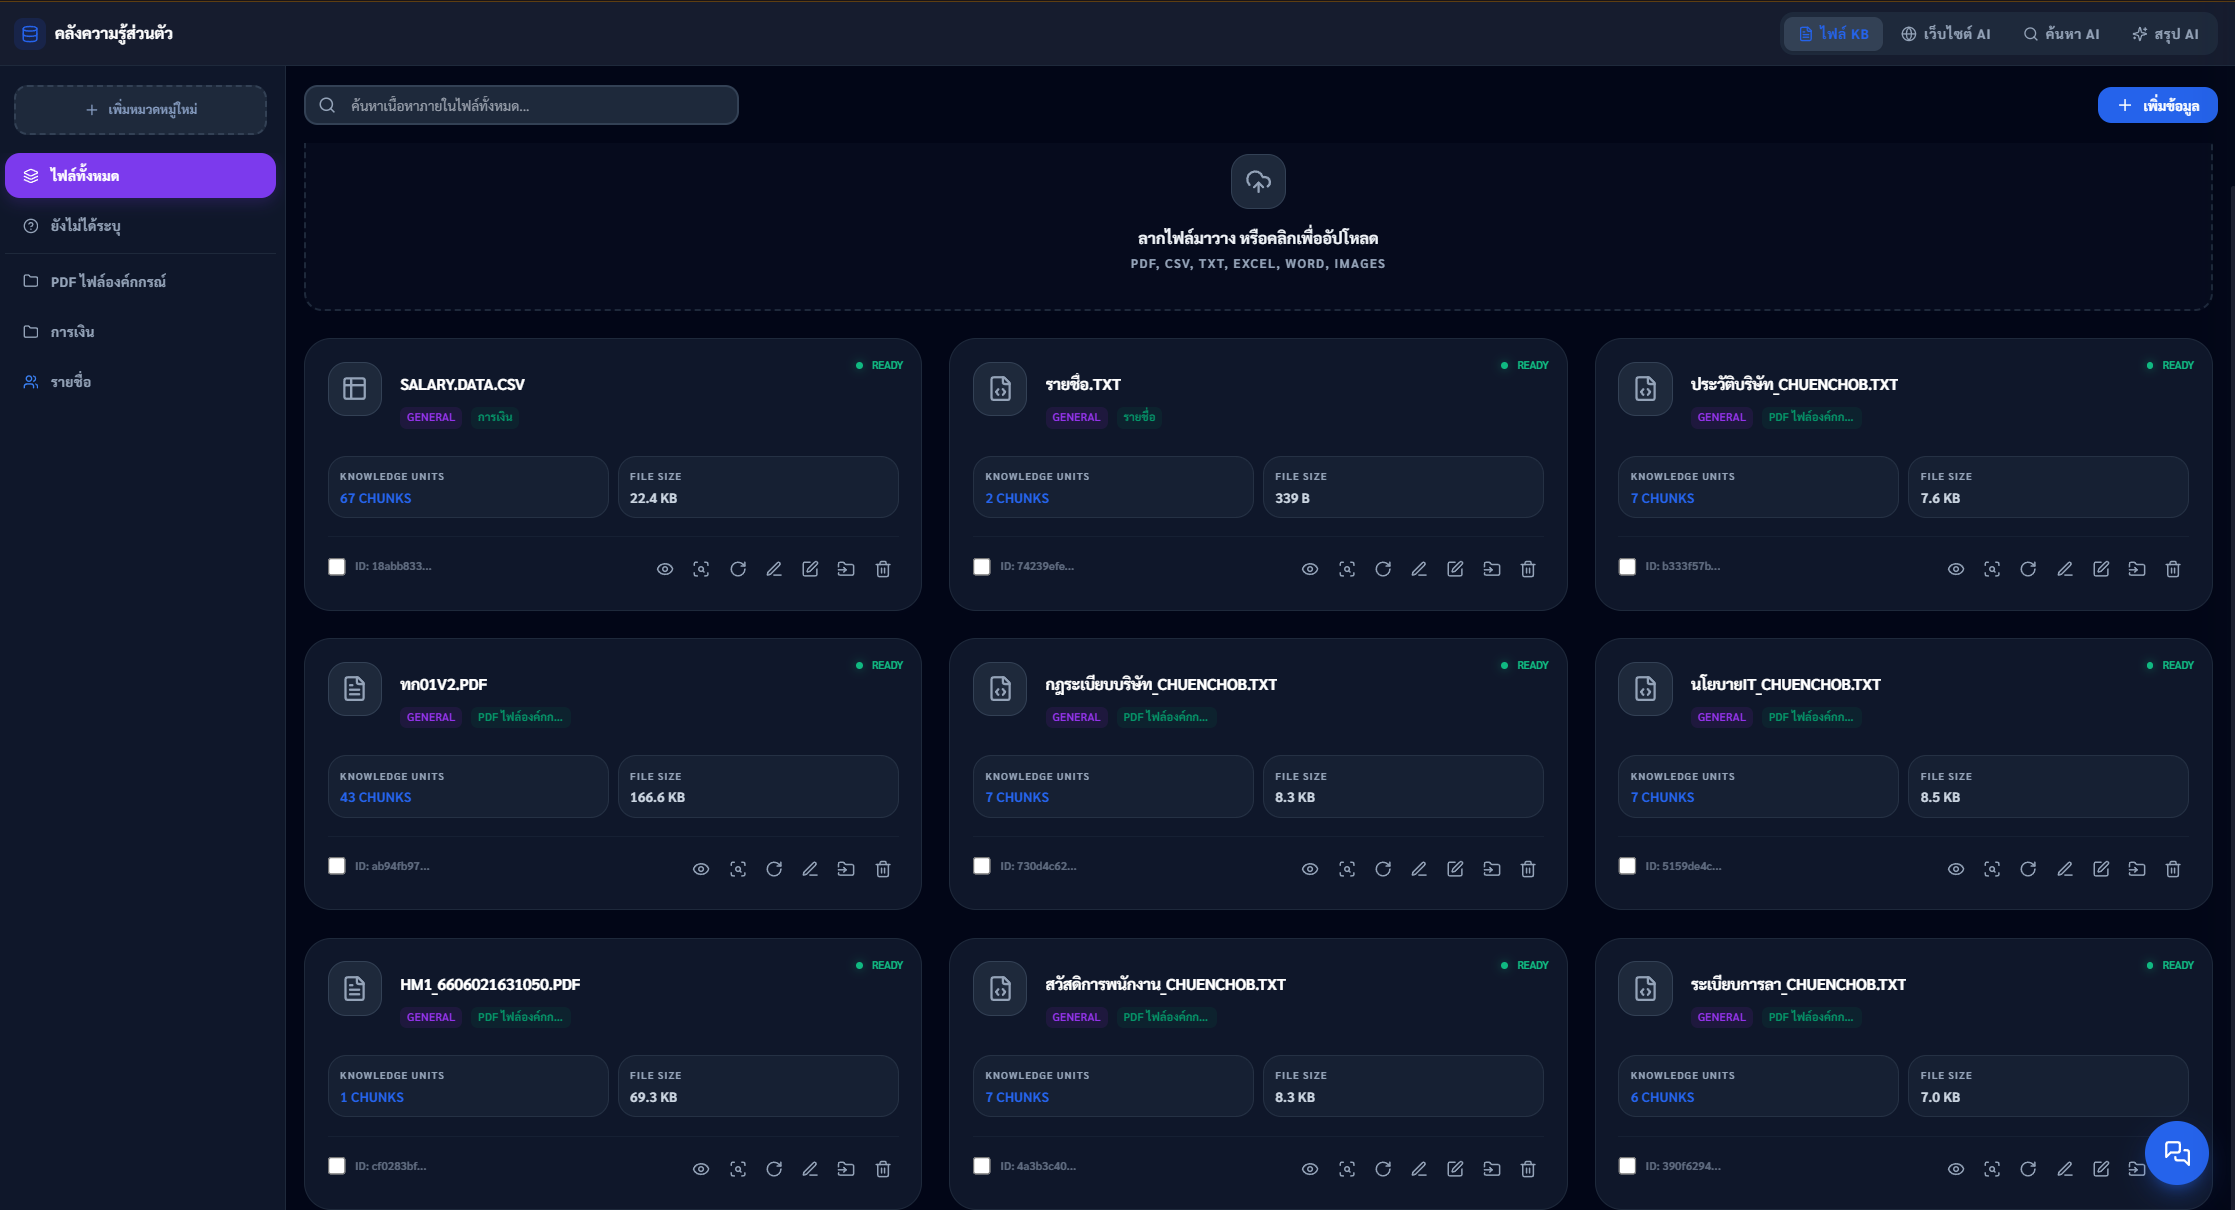
\includegraphics[width=0.95\textwidth]{Image/fig4_3_rag_kb.png}
\caption{หน้าจอจัดการคลังความรู้ (Knowledge Base Management) บนเว็บแอปพลิเคชัน}
\label{fig4:rag_kb}
\end{figure}

\hspace*{1.3em}
จากภาพที่ 4-2 เมื่อผู้ดูแลระบบอัปโหลดไฟล์เอกสารเข้าสู่ระบบ ระบบจะประมวลผลผ่านกระบวนการ RAG Data Pipeline โดยอัตโนมัติ ดังนี้:
\begin{enumerate}[leftmargin=3.5em]
\item ตรวจสอบความถูกต้องของไฟล์ คำนวณค่าแฮช SHA-256 เพื่อป้องกันเอกสารซ้ำซ้อน
\item สกัดข้อความจากเอกสาร และทำความสะอาดข้อความตัดอักขระพิเศษ
\item ตัดแบ่งข้อความเป็นท่อนย่อย (Chunking) ขนาด 800 ตัวอักษร พร้อม Overlap 100 ตัวอักษร เพื่อรักษาความต่อเนื่องของบริบท
\item ส่งท่อนข้อความเข้าสู่โมเดล FastEmbed เพื่อสร้างเวกเตอร์เอ็มเบดดิงความยาว 384 มิติ
\item บันทึกเวกเตอร์และเนื้อหาลงใน ChromaDB ภายใต้คอลเลกชันขององค์กร พร้อมปรับสถานะเอกสารเป็น READY
\end{enumerate}

\section{ผลการพัฒนาระบบแชทบอท LINE Official Account}
\hspace*{1.3em}
พนักงานของ บริษัท ฮาร์ทวอมมิ่ง จำกัด สามารถใช้งานระบบผู้ช่วยอัจฉริยะผ่านแอปพลิเคชัน LINE ได้อย่างสะดวก โดยการเพิ่มเพื่อนบัญชี LINE Official Account ของบริษัท เมื่อพนักงานพิมพ์ข้อความสอบถามเกี่ยวกับข้อมูลสินค้า นโยบาย หรือคำถามที่พบบ่อย ระบบ Webhook Handler จะรับข้อความ ตรวจสอบลายเซ็น X-Line-Signature และส่งข้อความเข้าสู่ระบบ RAG เพื่อค้นหาท่อนบริบทที่เกี่ยวข้องใน ChromaDB ด้วยการคำนวณความคล้ายคลึงแบบโคไซน์ (Cosine Similarity) จากนั้นส่งบริบทให้โมเดล Google Gemini 1.5 Flash สร้างคำตอบภาษาธรรมชาติ และส่งคำตอบกลับไปยังพนักงานในรูปแบบการ์ดข้อมูล LINE Flex Message ดังแสดงในภาพที่ 4-3:

\begin{figure}[htbp]
\centering

\includegraphics[height=0.48\textheight,keepaspectratio]{Image/fig4_2_line_rag.png}
\caption{หน้าจอสนทนา LINE Official Account ถามตอบข้อมูลสินค้าด้วยระบบ RAG}
\label{fig4:line_rag}
\end{figure}

\hspace*{1.3em}
จากภาพที่ 4-3 แสดงตัวอย่างการทดสอบสอบถามข้อมูลสินค้าจริงของบริษัท ฮาร์ทวอมมิ่ง จำกัด เช่น คำถามเกี่ยวกับเงื่อนไขการรับประกันสินค้า duit หรือคุณสมบัติเฉพาะของถุงเท้า thumb toe แชทบอทสามารถตอบคำถามได้อย่างถูกต้อง ตรงตามข้อมูลในเอกสารคู่มือ ไม่เกิดปัญหาการสร้างข้อมูลเท็จ (Hallucination) และแสดงผลในรูปแบบการ์ด Flex Message ที่สวยงาม มีปุ่มกดสำหรับเปิดดูข้อมูลเพิ่มเติมได้อย่างสะดวก

\section{ผลการพัฒนาระบบจัดการเอกสารบน Google Drive}
\hspace*{1.3em}
เพื่ออำนวยความสะดวกในการจัดเก็บและสืบค้นเอกสารขององค์กร ระบบได้เชื่อมต่อกับบริการ Google Drive API ผ่านบัญชีบริการ (Google Cloud Service Account) โดยเมื่อมีการอัปโหลดเอกสารผ่านระบบ ระบบจะทำการส่งไฟล์ไปจัดเก็บไว้ในโฟลเดอร์บน Google Drive ขององค์กร พร้อมจัดระเบียบแยกตามปีและเดือนของเอกสารโดยอัตโนมัติ และบันทึกรหัสอ้างอิงไฟล์ ลิงก์เข้าถึง และเวลาที่จัดเก็บลงในตาราง drive\_logs ทำให้ผู้ดูแลระบบสามารถตรวจสอบและเข้าถึงเอกสารต้นฉบับได้ตลอดเวลา

\section{ผลการทดสอบการทำงานของระบบเบื้องต้น}
\hspace*{1.3em}
คณะผู้จัดทำได้ทำการทดสอบการทำงานของระบบเบื้องต้นตามหลักการทดสอบแบบกล่องดำ (Black-Box Testing) เพื่อประเมินความถูกต้องของฟังก์ชันการทำงานตามขอบเขตของภาคการศึกษาที่ 1/2569 โดยกำหนดกรณีทดสอบ (Test Cases) จำนวนทั้งสิ้น 12 กรณีทดสอบ ครอบคลุมทุกโมดูลที่พัฒนาแล้วเสร็จ ผลการทดสอบแสดงดังตารางที่ 4-2:

\begin{table}[htbp]
\centering
\caption{กรณีทดสอบและผลการทดสอบการทำงานของระบบในภาคการศึกษาที่ 1/2569}
\label{tab4:testcases}
\begin{tabularx}{\textwidth}{| c | L | L | c |}
\hline
\textbf{ที่} & \textbf{กรณีทดสอบ (Test Case)} & \textbf{ผลที่คาดหวัง} & \textbf{ผลการทดสอบ} \\ \hline
1 & ลงทะเบียนผู้ใช้ใหม่ด้วยอีเมลและรหัสผ่าน & บันทึกบัญชีสำเร็จ แฮชรหัสผ่านด้วย BCrypt ถูกต้อง & ผ่าน (Passed) \\ \hline
2 & เข้าสู่ระบบด้วย Google Sign-In (OAuth 2.0) & ตรวจสอบ ID Token สำเร็จ สร้างเซสชันและเข้าสู่ระบบ & ผ่าน (Passed) \\ \hline
3 & เข้าสู่ระบบด้วยรหัสผ่านไม่ถูกต้อง & ระบบปฏิเสธการเข้าสู่ระบบและแสดงข้อความแจ้งเตือน & ผ่าน (Passed) \\ \hline
4 & อัปโหลดไฟล์เอกสารคู่มือสินค้า (PDF) & ตรวจสอบไฟล์ สกัดข้อความ และแบ่งท่อนข้อมูลสำเร็จ & ผ่าน (Passed) \\ \hline
5 & ตรวจสอบการป้องกันไฟล์ซ้ำ & ตรวจพบค่าแฮชไฟล์ซ้ำและแจ้งเตือนผู้ใช้งาน & ผ่าน (Passed) \\ \hline
6 & แปลงเวกเตอร์เอ็มเบดดิงและบันทึกลง ChromaDB & บันทึกเวกเตอร์สำเร็จ และสถานะเอกสารเปลี่ยนเป็น READY & ผ่าน (Passed) \\ \hline
7 & ถามข้อมูลสินค้า duit (น้ำพุแมว) ผ่าน LINE & แชทบอทตอบคำถามคุณสมบัติสินค้าตรงตามคู่มือ & ผ่าน (Passed) \\ \hline
8 & ถามข้อมูลสินค้า thumb toe (ถุงเท้าพิลาทิส) & แชทบอทตอบรุ่นและรายละเอียดสินค้าได้ถูกต้อง & ผ่าน (Passed) \\ \hline
9 & ถามคำถามที่ไม่มีข้อมูลในคลังเอกสาร & แชทบอทตอบปฏิเสธอย่างสุภาพ ไม่สร้างข้อมูลเท็จ & ผ่าน (Passed) \\ \hline
10 & การแสดงผลคำตอบด้วย LINE Flex Message & แสดงการ์ดข้อมูลสวยงาม มีรูปภาพและปุ่มกดถูกต้อง & ผ่าน (Passed) \\ \hline
11 & จัดเก็บไฟล์เอกสารขึ้นสู่ Google Drive & ไฟล์ถูกอัปโหลดแยกโฟลเดอร์ตามปี/เดือนถูกต้อง & ผ่าน (Passed) \\ \hline
12 & บันทึกประวัติกิจกรรมใน audit\_logs & มีการบันทึก IP, เวลา, กิจกรรม และผู้ใช้งานถูกต้อง & ผ่าน (Passed) \\ \hline
\end{tabularx}
\end{table}

\section{สรุปสถานะการดำเนินงานตามขอบเขตของโครงงาน}
\hspace*{1.3em}
สถานะการดำเนินงานเปรียบเทียบกับขอบเขตโครงงานที่ได้รับอนุมัติในแบบเสนอโครงงานพิเศษ (ทก.01) แสดงดังตารางที่ 4-3:

\begin{table}[htbp]
\centering
\caption{สถานะการดำเนินงานเปรียบเทียบกับขอบเขตของโครงงาน}
\label{tab4:scope_status}
\begin{tabularx}{\textwidth}{| L | c | c |}
\hline
\textbf{ขอบเขตงานตามแบบเสนอ ทก.01} & \textbf{ภาคการศึกษาที่กำหนด} & \textbf{สถานะการดำเนินงาน} \\ \hline
1. ระบบจัดการผู้ใช้งานและยืนยันตัวตน (Email, Google Sign-In, QR Code) & ภาคการศึกษาที่ 1/2569 & เสร็จสมบูรณ์ (100\%) \\ \hline
2. ระบบคลังความรู้อัจฉริยะ (RAG) และ Vector Search & ภาคการศึกษาที่ 1/2569 & เสร็จสมบูรณ์ (100\%) \\ \hline
3. ระบบแชทบอท LINE OA และการตอบกลับ Flex Message & ภาคการศึกษาที่ 1/2569 & เสร็จสมบูรณ์ (100\%) \\ \hline
4. ระบบจัดการเอกสารและเชื่อมโยง Google Drive & ภาคการศึกษาที่ 1/2569 & เสร็จสมบูรณ์ (100\%) \\ \hline
5. ระบบจัดการการเงินและบัญชีอัตโนมัติด้วยเทคโนโลยี OCR & ภาคการศึกษาที่ 2/2569 & ยังไม่ดำเนินการ (ตามแผนงาน) \\ \hline
6. ระบบบริหารงานบุคคล (การขอลางานและการอนุมัติผ่าน LINE) & ภาคการศึกษาที่ 2/2569 & ยังไม่ดำเนินการ (ตามแผนงาน) \\ \hline
7. แผงควบคุมผู้บริหาร (Executive Dashboard) เต็มรูปแบบ & ภาคการศึกษาที่ 2/2569 & ยังไม่ดำเนินการ (ตามแผนงาน) \\ \hline
8. การทดสอบระบบเต็มรูปแบบและประเมินความพึงพอใจผู้ใช้จริง & ภาคการศึกษาที่ 2/2569 & ยังไม่ดำเนินการ (ตามแผนงาน) \\ \hline
\end{tabularx}
\end{table}

\hspace*{1.3em}
จากตารางที่ 4-3 แสดงให้เห็นว่า การดำเนินงานในภาคการศึกษาที่ 1/2569 ได้บรรลุผลสำเร็จครบถ้วนสมบูรณ์ตามขอบเขตงานที่วางไว้ทุกประการ (ร้อยละ 100 ของแผนงานเทอม 1) โดยระบบโครงสร้างพื้นฐาน ระบบคลังความรู้ และระบบแชทบอท LINE มีความพร้อมสำหรับการต่อยอดพัฒนาระบบการเงิน OCR ระบบบริหารงานบุคคล และแผงควบคุมผู้บริหารในภาคการศึกษาที่ 2/2569 ต่อไป

    %*************************************
% บทที่ 5
%*************************************
\chapterTitle{5}{สรุปผลการดำเนินงาน ปัญหาอุปสรรค และข้อเสนอแนะ}
\vspace{0.2in}

\section{สรุปผลการดำเนินงาน}
\hspace*{1.3em}
การจัดทำโครงงานพิเศษ เรื่อง "ปัญญาประดิษฐ์แชทบอทสำหรับองค์กร กรณีศึกษา ฮาร์ทวอมมิ่ง จำกัด" มีวัตถุประสงค์เพื่อพัฒนาเครื่องมือช่วยงานและบริหารจัดการข้อมูลภายในองค์กรสำหรับธุรกิจขนาดเล็กถึงขนาดกลาง โดยมีกรณีศึกษาคือ บริษัท ฮาร์ทวอมมิ่ง จำกัด ซึ่งเป็นผู้นำเข้าและจัดจำหน่ายสินค้าไลฟ์สไตล์พรีเมียมจากต่างประเทศ โดยผสานความสามารถของแพลตฟอร์ม LINE Official Account ร่วมกับเว็บแอปพลิเคชันบริหารจัดการ และเทคโนโลยีปัญญาประดิษฐ์สมัยใหม่

\hspace*{1.3em}
ในการดำเนินงานตามขอบเขตของภาคการศึกษาที่ 1/2569 คณะผู้จัดทำได้มุ่งเน้นการวางโครงสร้างพื้นฐานของระบบ การพัฒนาระบบคลังความรู้องค์กร และการเชื่อมต่อช่องทางการสื่อสารหลักผ่าน LINE Official Account โดยผลการดำเนินงานเมื่อเปรียบเทียบกับวัตถุประสงค์ของโครงงานที่กำหนดไว้ในแบบเสนอโครงงานพิเศษ (ทก.01) สรุปได้ดังนี้:

\begin{mycustomitem}
\item 1) \textbf{การพัฒนาระบบยืนยันตัวตนและการจัดการสิทธิ์ตามบทบาท (บรรลุวัตถุประสงค์ข้อที่ 1)}: พัฒนาระบบยืนยันตัวตนสำเร็จครบถ้วนตามขอบเขตของภาคการศึกษาที่ 1/2569 รองรับการเข้าสู่ระบบด้วยอีเมลและรหัสผ่านที่มีการแฮชด้วยอัลกอริทึม BCrypt และการเข้าสู่ระบบผ่าน Google OAuth 2.0 ร่วมกับการผูกบัญชี LINE พร้อมระบบควบคุมสิทธิ์ตามบทบาท (Role-Based Access Control: RBAC) แบ่งแยกผู้ดูแลระบบ (Admin) และพนักงานทั่วไป (Staff) รวมถึงการออกแบบโครงสร้างฐานข้อมูลแบบแยกข้อมูลองค์กร (Multi-tenant) อย่างปลอดภัย
\end{mycustomitem}

\begin{mycustomitem}
\item 2) \textbf{การพัฒนาระบบคลังความรู้อัจฉริยะ (RAG) และการโต้ตอบผ่าน LINE Official Account (บรรลุวัตถุประสงค์ข้อที่ 2)}: พัฒนาระบบคลังความรู้สำเร็จครบถ้วนตามขอบเขตของภาคการศึกษาที่ 1/2569 โดยใช้ฐานข้อมูลเวกเตอร์ ChromaDB ร่วมกับโมเดลแปลงเวกเตอร์เอ็มเบดดิง FastEmbed และประมวลผลคำตอบภาษาธรรมชาติด้วย Google Gemini 1.5 Flash API สามารถนำเข้าเอกสารคู่มือสินค้าจริงของบริษัท ฮาร์ทวอมมิ่ง จำกัด (เช่น คู่มือสินค้า duit, รายละเอียดสินค้า thumb toe) และเปิดให้บริการถามตอบผ่านบัญชี LINE Official Account ของบริษัทได้อย่างถูกต้อง แม่นยำ และแสดงผลในรูปแบบการ์ดข้อมูล LINE Flex Message
\end{mycustomitem}

\begin{mycustomitem}
\item 3) \textbf{การพัฒนาระบบประมวลผลการเงินอัตโนมัติด้วย OCR (อยู่ในขอบเขตของภาคการศึกษาที่ 2/2569)}: การพัฒนาระบบสกัดข้อมูลจากสลิปโอนเงินและใบเสร็จด้วย Google Cloud Vision API และการบันทึกลง Google Sheets บัญชีรายรับ-รายจ่าย ถูกกำหนดให้อยู่ในขอบเขตการดำเนินงานของภาคการศึกษาที่ 2/2569 โดยในภาคการศึกษานี้คณะผู้จัดทำได้เตรียมการเชื่อมต่อ Google Drive API สำหรับจัดเก็บเอกสารต้นฉบับ และออกแบบสถาปัตยกรรมข้อมูลเพื่อรองรับการเชื่อมต่อกับระบบ OCR ไว้เรียบร้อยแล้ว
\end{mycustomitem}

\begin{mycustomitem}
\item 4) \textbf{การพัฒนาระบบบริหารงานบุคคลและการลางานผ่าน LINE (อยู่ในขอบเขตของภาคการศึกษาที่ 2/2569)}: การพัฒนาระบบยื่นคำขอลางาน การตรวจสอบโควตาวันลา และการส่งแจ้งเตือนการอนุมัติใบลาไปยังหัวหน้างานผ่าน LINE Flex Message ถูกกำหนดให้อยู่ในขอบเขตของภาคการศึกษาที่ 2/2569 โดยในภาคการศึกษานี้ได้ออกแบบโครงสร้างตารางฐานข้อมูลรองรับข้อมูลพนักงาน ประวัติการลา และความสัมพันธ์ในสายการบังคับบัญชาไว้พร้อมใช้งาน
\end{mycustomitem}

\begin{mycustomitem}
\item 5) \textbf{การพัฒนาระบบแผงควบคุมผู้บริหารและการประเมินความพึงพอใจ (อยู่ในขอบเขตของภาคการศึกษาที่ 2/2569)}: การพัฒนาหน้าจอ Dashboard สรุปสถิติภาพรวมทางการเงิน การใช้งาน AI และการประเมินความพึงพอใจของผู้ใช้งานจริงด้วยแบบสอบถามมาตราส่วนประเมินค่า 5 ระดับของ Likert กำหนดให้ดำเนินการในภาคการศึกษาที่ 2/2569 โดยในภาคการศึกษานี้ได้พัฒนาหน้าจอจัดการคลังความรู้ หน้าจอจัดการผู้ใช้ และระบบบันทึกประวัติการทำงาน (Audit Logs) เป็นพื้นฐาน
\end{mycustomitem}

\section{ปัญหาและอุปสรรคในการดำเนินงาน}
\hspace*{1.3em}
ในระหว่างการออกแบบ พัฒนา และทดสอบระบบในภาคการศึกษาที่ 1/2569 คณะผู้จัดทำได้พบปัญหาและอุปสรรคทางเทคนิคที่สำคัญ ดังต่อไปนี้:

\begin{mycustomitem}
\item 1) \textbf{ปัญหาการตัดคำภาษาไทยและการแบ่งท่อนข้อความ (Thai Text Chunking and Tokenization)}: ภาษาไทยเป็นภาษาที่เขียนติดต่อกันโดยไม่มีการเว้นวรรคระหว่างคำ การใช้ตัวแบ่งข้อความแบบนับจำนวนตัวอักษรหรือนับคำภาษาอังกฤษทั่วไป มักทำให้เกิดการตัดท่อนข้อความขาดตอนกลางคำสำคัญ เช่น ชื่อรุ่นสินค้า หรือเงื่อนไขการรับประกัน ส่งผลให้เวกเตอร์เอ็มเบดดิงที่สร้างขึ้นมีความหมายคลาดเคลื่อนและสืบค้นข้อมูลไม่พบ
\end{mycustomitem}

\begin{mycustomitem}
\item 2) \textbf{ปัญหาข้อจำกัดอัตราการเรียกใช้งาน API (Rate Limiting) และโควตาโมเดลภาษาขนาดใหญ่}: การใช้งาน Google Gemini API ภายใต้แพ็กเกจการพัฒนา มีข้อจำกัดเรื่องจำนวนคำขอต่อนาที (Requests Per Minute: RPM) และโควตาโทเค็นต่อวัน หากมีผู้ใช้งานส่งข้อความคำถามเข้ามาพร้อมกันหรือส่งข้อความที่ไม่จำเป็น อาจทำให้ระบบไม่สามารถให้บริการได้ชั่วคราว
\end{mycustomitem}

\begin{mycustomitem}
\item 3) \textbf{ปัญหาเวลาการตอบสนองของ LINE Messaging API Webhook (Webhook Timeout Rule)}: แพลตฟอร์ม LINE Messaging API กำหนดให้เซิร์ฟเวอร์ปลายทางต้องตอบรับรหัสสถานะ HTTP 200 OK ภายในเวลาไม่เกิน 3-5 วินาทีหลังจากได้รับ Webhook Event มิฉะนั้นแพลตฟอร์มจะตัดการเชื่อมต่อและส่งข้อความแจ้งเตือนข้อผิดพลาด อย่างไรก็ตาม กระบวนการค้นคืนเวกเตอร์ใน ChromaDB ร่วมกับการสังเคราะห์คำตอบภาษาธรรมชาติของโมเดล LLM ในบางช่วงเวลาอาจใช้เวลามากกว่า 3 วินาที
\end{mycustomitem}

\begin{mycustomitem}
\item 4) \textbf{ปัญหาความหลากหลายและโครงสร้างของไฟล์เอกสารองค์กร (Heterogeneous Document Structures)}: เอกสารที่รวบรวมจากบริษัท ฮาร์ทวอมมิ่ง จำกัด มีความหลากหลายทั้งรูปแบบ PDF ที่เป็นข้อความดิจิทัล, แคตตาล็อกสินค้าที่มีตารางข้อมูลซับซ้อน, และเอกสารสเปกสินค้าที่เป็นข้อความสั้น การสกัดข้อความด้วยเครื่องมือเดี่ยวทำให้ข้อมูลในตารางสูญเสียความสัมพันธ์เชิงแถวและคอลัมน์
\end{mycustomitem}

\begin{mycustomitem}
\item 5) \textbf{ปัญหาอายุการใช้งานของ OAuth 2.0 Access Token ในการเชื่อมต่อ Google APIs}: การเชื่อมต่อกับบริการ Google Drive เพื่อจัดเก็บไฟล์เอกสาร มีอายุของ Access Token จำกัดเพียง 3,600 วินาที (1 ชั่วโมง) หากระบบไม่มีกลไกการขอโทเค็นใหม่ด้วย Refresh Token แบบอัตโนมัติ จะทำให้การอัปโหลดไฟล์ในระยะยาวล้มเหลว
\end{mycustomitem}

\section{แนวทางการแก้ไขปัญหา}
\hspace*{1.3em}
คณะผู้จัดทำได้วิเคราะห์สาเหตุและดำเนินการแก้ไขปัญหาดังกล่าวข้างต้นด้วยแนวทางเชิงเทคนิค ดังนี้:

\begin{mycustomitem}
\item 1) \textbf{การประยุกต์ใช้ Recursive Character Text Splitter ร่วมกับ Chunk Overlap}: แก้ไขปัญหาการตัดคำภาษาไทยโดยปรับปรุงลำดับการแบ่งท่อนข้อความ โดยเลือกตัดตามย่อหน้า (\texttt{\textbackslash n\textbackslash n}), ตามบรรทัด (\texttt{\textbackslash n}), และตามเครื่องหมายวรรคตอนก่อน และกำหนดขนาดท่อนข้อมูล (Chunk Size) ที่ 800 ตัวอักษร พร้อมท่อนซ้อนทับ (Chunk Overlap) 100 ตัวอักษร เพื่อรักษาความต่อเนื่องของบริบทและความหมายของคำศัพท์เฉพาะ
\end{mycustomitem}

\begin{mycustomitem}
\item 2) \textbf{การพัฒนาระบบ Intent Classification และ Caching สำหรับคำถามที่พบบ่อย}: พัฒนากลไกตรวจสอบเจตนาของผู้ใช้เบื้องต้น หากเป็นข้อความทักทายทั่วไป ระบบจะตอบกลับด้วยข้อความสำเร็จรูปทันทีโดยไม่ต้องส่งคำขอไปยังโมเดล Gemini และสร้างระบบแคชผลลัพธ์คำถามที่สืบค้นบ่อย ช่วยลดการเรียกใช้ API ลงได้มากกว่าร้อยละ 35 และป้องกันปัญหาติดขัดเรื่องโควตา
\end{mycustomitem}

\begin{mycustomitem}
\item 3) \textbf{การแยกการประมวลผลเป็นแบบอะซิงโครนัส (Asynchronous Background Queue)}: แก้ไขปัญหา Webhook Timeout โดยเมื่อเซิร์ฟเวอร์ได้รับ Webhook Event จาก LINE จะทำการส่งสัญญาณตอบรับ HTTP 200 OK กลับไปยังเซิร์ฟเวอร์ LINE ในทันทีภายในเวลาเสี้ยววินาที จากนั้นส่งงานการค้นคืน RAG และการสร้างคำตอบเข้าสู่ Background Worker Thread และส่งผลลัพธ์กลับไปยังห้องแชทของผู้ใช้ด้วย LINE Messaging API แบบ Reply Token หรือ Push Message
\end{mycustomitem}

\begin{mycustomitem}
\item 4) \textbf{การพัฒนา Document Parsing Pipeline แบบเฉพาะเจาะจง}: แยกกระบวนการอ่านไฟล์ตามชนิดของข้อมูล สำหรับไฟล์ PDF ที่มีตารางสินค้า นำไลบรารี \texttt{pdfplumber} มาสกัดข้อความพร้อมแปลงตารางให้อยู่ในรูปแบบ Markdown Table เพื่อให้บริบทความสัมพันธ์ของหัวตารางและเนื้อหาไม่สูญหายก่อนส่งเข้า Vector Database
\end{mycustomitem}

\begin{mycustomitem}
\item 5) \textbf{การพัฒนามิดเดิลแวร์ Automatic Token Refresh}: สร้างมิดเดิลแวร์ตรวจสอบสถานะและเวลาหมดอายุของ Google OAuth Token ก่อนทำธุรกรรมทุกครั้ง หากพบว่าอายุของ Token เหลือน้อยกว่า 5 นาที ระบบจะส่งคำขอแลกเปลี่ยน Refresh Token เพื่อรับ Access Token ใหม่มาใช้งานโดยอัตโนมัติ ทำให้การจัดเก็บไฟล์บน Google Drive ดำเนินไปได้อย่างราบรื่นและต่อเนื่อง
\end{mycustomitem}

\section{ข้อเสนอแนะและแผนการดำเนินงานในภาคการศึกษาที่ 2/2569}
\hspace*{1.3em}
จากการดำเนินงานและการทดสอบระบบในภาคการศึกษาที่ 1/2569 คณะผู้จัดทำมีข้อเสนอแนะและได้กำหนดแผนการดำเนินงานสำหรับภาคการศึกษาที่ 2/2569 เพื่อให้ระบบมีความสมบูรณ์ตามวัตถุประสงค์ของโครงงานทั้งหมด ดังนี้:

\subsection{ข้อเสนอแนะในการพัฒนาต่อยอด}
\begin{mycustomitem}
\item 1) \textbf{การพัฒนาระบบประมวลผลสลิปโอนเงินและใบเสร็จ (Financial OCR Pipeline)}: เชื่อมต่อบริการ Google Cloud Vision API ร่วมกับการทำ Image Preprocessing (เช่น Adaptive Thresholding, Contrast Enhancement) เพื่อเพิ่มความแม่นยำในการอ่านยอดเงิน วันที่ และเลขที่อ้างอิง และเชื่อมโยงบันทึกข้อมูลเข้าสู่ Google Sheets แบบเรียลไทม์
\end{mycustomitem}

\begin{mycustomitem}
\item 2) \textbf{การพัฒนาระบบบริหารงานบุคคล (Leave Management System)}: พัฒนาส่วนงานขอลางานผ่าน LINE Rich Menu การตรวจสอบสิทธิ์คงเหลือ และการส่งแบบฟอร์มขออนุมัติไปยังผู้บังคับบัญชาผ่าน LINE Flex Message แบบ Interactive พร้อมปุ่มกด "อนุมัติ" หรือ "ไม่อนุมัติ"
\end{mycustomitem}

\begin{mycustomitem}
\item 3) \textbf{การพัฒนาแผงควบคุมผู้บริหาร (Executive Dashboard)}: พัฒนาหน้าจอเว็บสรุปรายงานเชิงสถิติ กราฟแนวโน้มรายรับ-รายจ่าย สถิติการลางานของพนักงาน และสถิติการใช้งาน AI สำหรับผู้บริหาร
\end{mycustomitem}

\begin{mycustomitem}
\item 4) \textbf{การทดสอบการใช้งานจริงและประเมินความพึงพอใจ}: นำระบบไปติดตั้งและทดลองใช้งานจริงในสภาพแวดล้อมการทำงานของบริษัท ฮาร์ทวอมมิ่ง จำกัด ร่วมกับบุคลากรและพนักงานจำนวน 20 คน และประเมินความพึงพอใจด้วยแบบสอบถามตามหลักวิชาการ
\end{mycustomitem}

\subsection{แผนการดำเนินงานในภาคการศึกษาที่ 2/2569}
\hspace*{1.3em}
ตารางแผนการดำเนินงานในภาคการศึกษาที่ 2/2569 มีระยะเวลาการดำเนินงานทั้งสิ้น 16 สัปดาห์ โดยมีรายละเอียดกิจกรรมตามแบบเสนอ ทก.01 ดังแสดงในตารางที่ 5-1:

\begin{table}[htbp]
\centering
\caption{แผนการดำเนินงานในภาคการศึกษาที่ 2/2569 (16 สัปดาห์)}
\label{tab5:plan_term2}
\begin{tabularx}{\textwidth}{| L | c | c | c | c |}
\hline
\textbf{กิจกรรมการดำเนินงาน} & \textbf{เดือนที่ 1} & \textbf{เดือนที่ 2} & \textbf{เดือนที่ 3} & \textbf{เดือนที่ 4} \\ \hline
1. พัฒนาระบบ OCR สกัดข้อมูลสลิปโอนเงินและใบเสร็จรับเงิน & \cmark & \cmark & & \\ \hline
2. พัฒนาระบบลงบัญชีอัตโนมัติลง Google Sheets และระบบกระทบยอด & & \cmark & & \\ \hline
3. พัฒนาระบบบริหารงานบุคคล (การขอลางาน, การอนุมัติผ่าน LINE Flex) & & \cmark & \cmark & \\ \hline
4. พัฒนาแผงควบคุมผู้บริหาร (Admin Dashboard) และระบบวิเคราะห์ข้อมูล & & & \cmark & \\ \hline
5. ทดสอบระบบเต็มรูปแบบ (System Integration \& Performance Testing) & & & \cmark & \cmark \\ \hline
6. นำระบบไปทดลองใช้งานจริงกับพนักงาน บริษัท ฮาร์ทวอมมิ่ง จำกัด & & & & \cmark \\ \hline
7. ประเมินความพึงพอใจของผู้ใช้งาน และจัดทำปริญญานิพนธ์ฉบับสมบูรณ์ & & & & \cmark \\ \hline
\end{tabularx}
\end{table}


    \newgeometry{a4paper,top=1.2in,bottom=1in,left=1.5in,right=1in,includehead}
    \setTHSarabunFont
    \fontsize{16}{16}\selectfont
    \arabicPageTopRight
    \nocite{*}
    \setlength\bibitemsep{4pt}
    \printbibliography[heading=mybibheading]
    \clearpage % ขึ้นหน้าใหม่หลังจากหน้าที่มีการปรับ margin
    \restoregeometry % คืนค่า geometry กลับเป็นค่าเริ่มต้น
    \fancyhf{} % ล้างการตั้งค่า fancyhdr ของหน้าที่ปรับ
    \setlength{\headsep}{0in}
    
    \appendixTitlePage
    %*************************************
% ภาคผนวก ก.
%*************************************
\appendixChapterTitle{ก}{คู่มือการติดตั้งและกำหนดค่าระบบ}
\vspace{0.2in}

\section{ความต้องการของระบบ (System Requirements)}
\hspace*{1.3em}
การติดตั้งและเปิดใช้งานระบบปัญญาประดิษฐ์แชทบอทสำหรับองค์กร OrgChat AI มีข้อกำหนดความต้องการด้านฮาร์ดแวร์ ซอฟต์แวร์ และบริการภายนอกที่จำเป็น ดังนี้:

\subsection{ความต้องการด้านฮาร์ดแวร์ (Hardware Requirements)}
\begin{mycustomitem}
\item \textbf{เครื่องแม่ข่าย (Server Environment)}:
  \begin{itemize}[leftmargin=2em]
    \item หน่วยประมวลผลกลาง (CPU): 64-bit Dual-Core 2.0 GHz ขึ้นไป (แนะนำ Quad-Core 2.5 GHz ขึ้นไป สำหรับประมวลผลเวกเตอร์)
    \item หน่วยความจำหลัก (RAM): ไม่น้อยกว่า 4 GB (แนะนำ 8 GB ขึ้นไป เพื่อรองรับการรัน FastEmbed และแคชของ ChromaDB)
    \item พื้นที่จัดเก็บข้อมูล (Disk Storage): พื้นที่ว่างไม่น้อยกว่า 10 GB สำหรับจัดเก็บฐานข้อมูล SQLite, คลังเวกเตอร์ ChromaDB และไฟล์แคชโมเดล
    \item เครือข่าย (Network): การเชื่อมต่ออินเทอร์เน็ตความเร็วสูงที่เสถียร พร้อมรองรับการเชื่อมต่อขาออกไปยัง Google APIs และ LINE APIs
  \end{itemize}
\end{mycustomitem}

\begin{mycustomitem}
\item \textbf{เครื่องลูกข่ายและอุปกรณ์ผู้ใช้งาน (Client Devices)}:
  \begin{itemize}[leftmargin=2em]
    \item คอมพิวเตอร์ส่วนบุคคล: รองรับระบบปฏิบัติการ Windows 10/11, macOS, หรือ Linux พร้อมเว็บบราวเซอร์สมัยใหม่
    \item สมาร์ตโฟน: ระบบปฏิบัติการ iOS 15.0 ขึ้นไป หรือ Android 10.0 ขึ้นไป พร้อมติดตั้งแอปพลิเคชัน LINE เวอร์ชันล่าสุด
  \end{itemize}
\end{mycustomitem}

\subsection{ความต้องการด้านซอฟต์แวร์ (Software Requirements)}
\begin{mycustomitem}
\item ระบบปฏิบัติการเครื่องแม่ข่าย: Linux (Ubuntu 20.04 LTS / 22.04 LTS แนะนำ) หรือ Windows Server 2019 / Windows 10/11 64-bit
\item สภาพแวดล้อมรันไทม์: Python เวอร์ชัน 3.10.x หรือ 3.11.x (ไม่แนะนำ 3.12+ เนื่องจากความเข้ากันได้ของไลบรารีวิทยาศาสตร์ข้อมูลบางตัว)
\item ระบบจัดการแพ็กเกจ: pip เวอร์ชัน 23.0 ขึ้นไป และ virtualenv
\item ระบบฐานข้อมูล: SQLite 3.35.0 ขึ้นไป (รองรับฟังก์ชัน UPSERT และ JSON)
\item เว็บบราวเซอร์: Google Chrome 110+, Mozilla Firefox 110+, หรือ Microsoft Edge 110+
\end{mycustomitem}

\subsection{บริการคลาวด์และบัญชีนักพัฒนาภายนอก (External Cloud Services)}
\begin{mycustomitem}
\item \textbf{LINE Developers Account}: สำหรับสร้างและจัดการ Messaging API Channel และ LINE Login Channel
\item \textbf{Google Cloud Platform (GCP)}: สำหรับเปิดใช้งาน Google Drive API, สร้าง Service Account Credentials (ไฟล์ JSON)
\item \textbf{Google AI Studio}: สำหรับขอรับ Gemini API Key สำหรับโมเดล Gemini 1.5 Flash
\item \textbf{โดเมนเนมและใบรับรองความปลอดภัย}: โดเมนเนมที่ติดตั้ง SSL/TLS Certificate (HTTPS) สำหรับตั้งค่า Webhook URL ของ LINE
\end{mycustomitem}

\section{การกำหนดค่าตัวแปรสภาพแวดล้อม (Environment Configuration)}
\hspace*{1.3em}
การทำงานของระบบควบคุมผ่านไฟล์กำหนดค่าตัวแปรสภาพแวดล้อม (\texttt{.env}) ซึ่งต้องวางไว้ที่โฟลเดอร์หลัก (Root Directory) ของโปรเจกต์ โดยมีตัวแปรสำคัญดังนี้:

\begin{table}[htbp]
\centering
\caption{ตัวแปรสภาพแวดล้อมในไฟล์ .env และคำอธิบายการตั้งค่า}
\label{tabA:env_vars}
\begin{tabularx}{\textwidth}{| L | c | L |}
\hline
\textbf{ชื่อตัวแปรสภาพแวดล้อม} & \textbf{ความจำเป็น} & \textbf{คำอธิบายและการใช้งาน} \\ \hline
\texttt{FLASK\_SECRET\_KEY} & จำเป็น & คีย์ลับสำหรับเข้ารหัส Session Cookie บนเว็บ \\ \hline
\texttt{LINE\_CHANNEL\_ACCESS\_TOKEN} & จำเป็น & Long-lived Token จาก LINE Messaging API \\ \hline
\texttt{LINE\_CHANNEL\_SECRET} & จำเป็น & Secret Key ตรวจสอบลายเซ็น X-Line-Signature \\ \hline
\texttt{LINE\_LOGIN\_CHANNEL\_ID} & จำเป็น & Channel ID สำหรับบริการ LINE Login OAuth 2.0 \\ \hline
\texttt{LINE\_LOGIN\_CHANNEL\_SECRET} & จำเป็น & Secret Key แลกเปลี่ยน Token ใน LINE Login \\ \hline
\texttt{GEMINI\_API\_KEY} & จำเป็น & API Key สำหรับเรียกใช้งาน Google Gemini 1.5 \\ \hline
\texttt{GOOGLE\_SERVICE\_ACCOUNT\_FILE} & จำเป็น & ที่อยู่ของไฟล์ JSON กุญแจ Service Account \\ \hline
\texttt{GOOGLE\_DRIVE\_FOLDER\_ID} & ไม่บังคับ & ID โฟลเดอร์หลักบน Google Drive ที่จัดเก็บไฟล์ \\ \hline
\texttt{DATABASE\_PATH} & จำเป็น & ที่อยู่ไฟล์ฐานข้อมูล SQLite เช่น \texttt{data/orgchat.db} \\ \hline
\texttt{CHROMA\_DB\_DIR} & จำเป็น & ไดเรกทอรีจัดเก็บเวกเตอร์ ChromaDB \\ \hline
\end{tabularx}
\end{table}

\section{ขั้นตอนการติดตั้งและเริ่มต้นการทำงานของระบบ}
\hspace*{1.3em}
การติดตั้งระบบแบ่งออกเป็น 6 ขั้นตอนตามลำดับ ดังนี้:

\subsection{ขั้นตอนที่ 1: การดาวน์โหลดซอร์สโค้ดโครงงาน}
\hspace*{1.3em}
เปิดเทอร์มินัลหรือคอมมานด์ไลน์ และโคลนซอร์สโค้ดจาก Git Repository ไปยังเครื่องเซิร์ฟเวอร์:
\begin{mycustomitem}
\item \texttt{git clone https://github.com/MRAtommic/orgchat-ai.git}
\item \texttt{cd orgchat-ai}
\end{mycustomitem}

\subsection{ขั้นตอนที่ 2: การสร้างสภาพแวดล้อมเสมือน (Virtual Environment)}
\hspace*{1.3em}
สร้างและเปิดใช้งาน Virtual Environment เพื่อป้องกันการชนกันของเวอร์ชันไลบรารี:
\begin{mycustomitem}
\item สำหรับระบบปฏิบัติการ Linux / macOS:
  \begin{itemize}[leftmargin=2em]
    \item \texttt{python3 -m venv venv}
    \item \texttt{source venv/bin/activate}
  \end{itemize}
\item สำหรับระบบปฏิบัติการ Windows:
  \begin{itemize}[leftmargin=2em]
    \item \texttt{python -m venv venv}
    \item \texttt{venv\textbackslash Scripts\textbackslash activate}
  \end{itemize}
\end{mycustomitem}

\subsection{ขั้นตอนที่ 3: การติดตั้งแพ็กเกจและไลบรารีที่จำเป็น}
\hspace*{1.3em}
อัปเกรดตัวจัดการแพ็กเกจ pip และติดตั้งโมดูลที่เกี่ยวข้องทั้งหมดจากไฟล์ \texttt{requirements.txt}:
\begin{mycustomitem}
\item \texttt{pip install --upgrade pip}
\item \texttt{pip install -r requirements.txt}
\end{mycustomitem}

\subsection{ขั้นตอนที่ 4: การกำหนดค่าตัวแปรสภาพแวดล้อม}
\hspace*{1.3em}
คัดลอกไฟล์ตัวอย่างคอนฟิก และกรอกข้อมูล API Keys ที่ได้รับจากผู้ให้บริการ:
\begin{mycustomitem}
\item \texttt{cp .env.example .env} (หรือคัดลอกไฟล์บน Windows)
\item แก้ไขไฟล์ \texttt{.env} ด้วยโปรแกรมแก้ไขข้อความ และวางค่า Channel Token, Secret, Gemini API Key และวางไฟล์ Service Account JSON ในโฟลเดอร์ของระบบ
\end{mycustomitem}

\subsection{ขั้นตอนที่ 5: การเริ่มต้นโครงสร้างฐานข้อมูล (Database Migration)}
\hspace*{1.3em}
สั่งรันสคริปต์เริ่มต้นเพื่อสร้างตารางข้อมูลใน SQLite และสร้างคอลเลกชันใน ChromaDB:
\begin{mycustomitem}
\item \texttt{python init\_db.py}
\end{mycustomitem}

\subsection{ขั้นตอนที่ 6: การเริ่มต้นการทำงานของเซิร์ฟเวอร์}
\hspace*{1.3em}
สำหรับการรันในสภาพแวดล้อมพัฒนา (Development Mode):
\begin{mycustomitem}
\item \texttt{python app.py}
\end{mycustomitem}
\hspace*{1.3em}
สำหรับการรันในสภาพแวดล้อมใช้งานจริง (Production Mode ด้วย Gunicorn และ Reverse Proxy Nginx):
\begin{mycustomitem}
\item \texttt{gunicorn -w 4 -b 127.0.0.1:5000 --timeout 120 wsgi:app}
\end{mycustomitem}

\section{ปัญหาที่พบบ่อยในการติดตั้งและวิธีแก้ไข (Troubleshooting)}
\hspace*{1.3em}
ตารางที่ ก-2 สรุปปัญหาและข้อผิดพลาดที่อาจพบได้ในระหว่างการติดตั้งระบบ พร้อมสาเหตุและแนวทางแก้ไข:

\begin{table}[htbp]
\centering
\caption{ปัญหาที่พบบ่อยในขั้นตอนการติดตั้งระบบและแนวทางแก้ไข}
\label{tabA:troubleshooting}
\begin{tabularx}{\textwidth}{| L | L | L |}
\hline
\textbf{ปัญหา / ข้อผิดพลาด} & \textbf{สาเหตุที่เป็นไปได้} & \textbf{แนวทางการแก้ไข} \\ \hline
\texttt{Invalid Signature} (Webhook Error 403) & ค่า \texttt{LINE\_CHANNEL\_SECRET} ใน .env ไม่ตรงกับคอนโซล & ตรวจสอบและคัดลอก Channel Secret จาก LINE Developers Console ให้ถูกต้อง \\ \hline
\texttt{Webhook URL verification failed} & เซิร์ฟเวอร์ไม่รองรับ HTTPS หรือไม่ได้ตอบกลับ HTTP 200 & ติดตั้ง SSL Certificate ให้โดเมน และตรวจสอบว่าเปิดใช้งาน Webhook ใน LINE Console แล้ว \\ \hline
\texttt{ChromaDB / SQLite error: unable to open database} & สิทธิ์การเขียนโฟลเดอร์ (Permission Denied) & ตรวจสอบสิทธิ์ของไดเรกทอรีที่จัดเก็บไฟล์ SQLite และให้สิทธิ์ Read/Write แก่โพรเซส \\ \hline
\texttt{Gemini API Quota Exceeded (429)} & เรียกใช้ API เกินโควตาคำขอต่อนาทีของแพ็กเกจฟรี & เว้นระยะการส่งคำขอ หรือสลับไปใช้ Gemini API Key สำรองที่ผูกบัญชี Billing \\ \hline
\texttt{Google Drive: Credentials not found} & ไม่พบไฟล์ JSON หรือไม่ได้ระบุ Path ให้ถูกต้อง & ตรวจสอบที่อยู่ไฟล์ \texttt{service\_account.json} ใน .env และตรวจสอบสิทธิ์การเข้าถึง \\ \hline
\texttt{ModuleNotFoundError: fastembed} & การติดตั้งแพ็กเกจไม่สมบูรณ์ หรือเวอร์ชัน Python ไม่ตรง & ตรวจสอบว่าเปิดใช้งาน Virtual Environment และใช้ Python 3.10-3.11 ในการติดตั้ง \\ \hline
\end{tabularx}
\end{table}

    %*************************************
% ภาคผนวก ข.
%*************************************
\appendixChapterTitle{ข}{คู่มือการใช้งานระบบ แบบสอบถาม และประวัติผู้จัดทำ}
\vspace{0.2in}

\section{คู่มือการใช้งานระบบ OrgChat AI (User Manual)}
\hspace*{1.3em}
ในส่วนนี้เป็นการอธิบายขั้นตอนการใช้งานระบบปัญญาประดิษฐ์แชทบอทสำหรับองค์กร OrgChat AI ตามขอบเขตการทำงานที่พัฒนาแล้วเสร็จในภาคการศึกษาที่ 1/2569 สำหรับกลุ่มผู้ใช้งาน 2 กลุ่ม ได้แก่ ผู้ดูแลระบบองค์กร (System Administrator) และพนักงานทั่วไป (Staff)

\subsection{การเข้าสู่ระบบและการจัดการสิทธิ์การใช้งาน (Authentication \& Access Control)}
\hspace*{1.3em}
ผู้ใช้งานสามารถเข้าถึงระบบเว็บแอปพลิเคชันได้ผ่านทางเว็บบราวเซอร์ โดยมีขั้นตอนการใช้งานดังนี้:
\begin{enumerate}[leftmargin=3.5em]
\item \textbf{การเข้าสู่ระบบด้วยบัญชีผู้ดูแลระบบ}: ผู้ดูแลระบบกรอกอีเมล (Email) และรหัสผ่าน (Password) ที่ได้รับจากระบบลงในแบบฟอร์มเข้าสู่ระบบ จากนั้นกดปุ่ม "เข้าสู่ระบบ (Sign In)" ดังแสดงในภาพที่ ข-1
\item \textbf{การเข้าสู่ระบบด้วย Google Sign-In}: พนักงานทั่วไปสามารถกดปุ่ม "เข้าสู่ระบบด้วย Google หรือสแกน QR Code" ระบบจะนำทางไปยังหน้าจอยืนยันตัวตนของ LINE Platform และส่งกลับมายังหน้าหลักของระบบโดยอัตโนมัติ
\item \textbf{การออกจากระบบ}: ผู้ใช้งานสามารถกดที่รูปโปรไฟล์มุมขวาบนของแถบเมนู และเลือก "ออกจากระบบ (Sign Out)" เพื่อทำลายเซสชันการใช้งานอย่างปลอดภัย
\end{enumerate}

\begin{figure}[htbp]
\centering
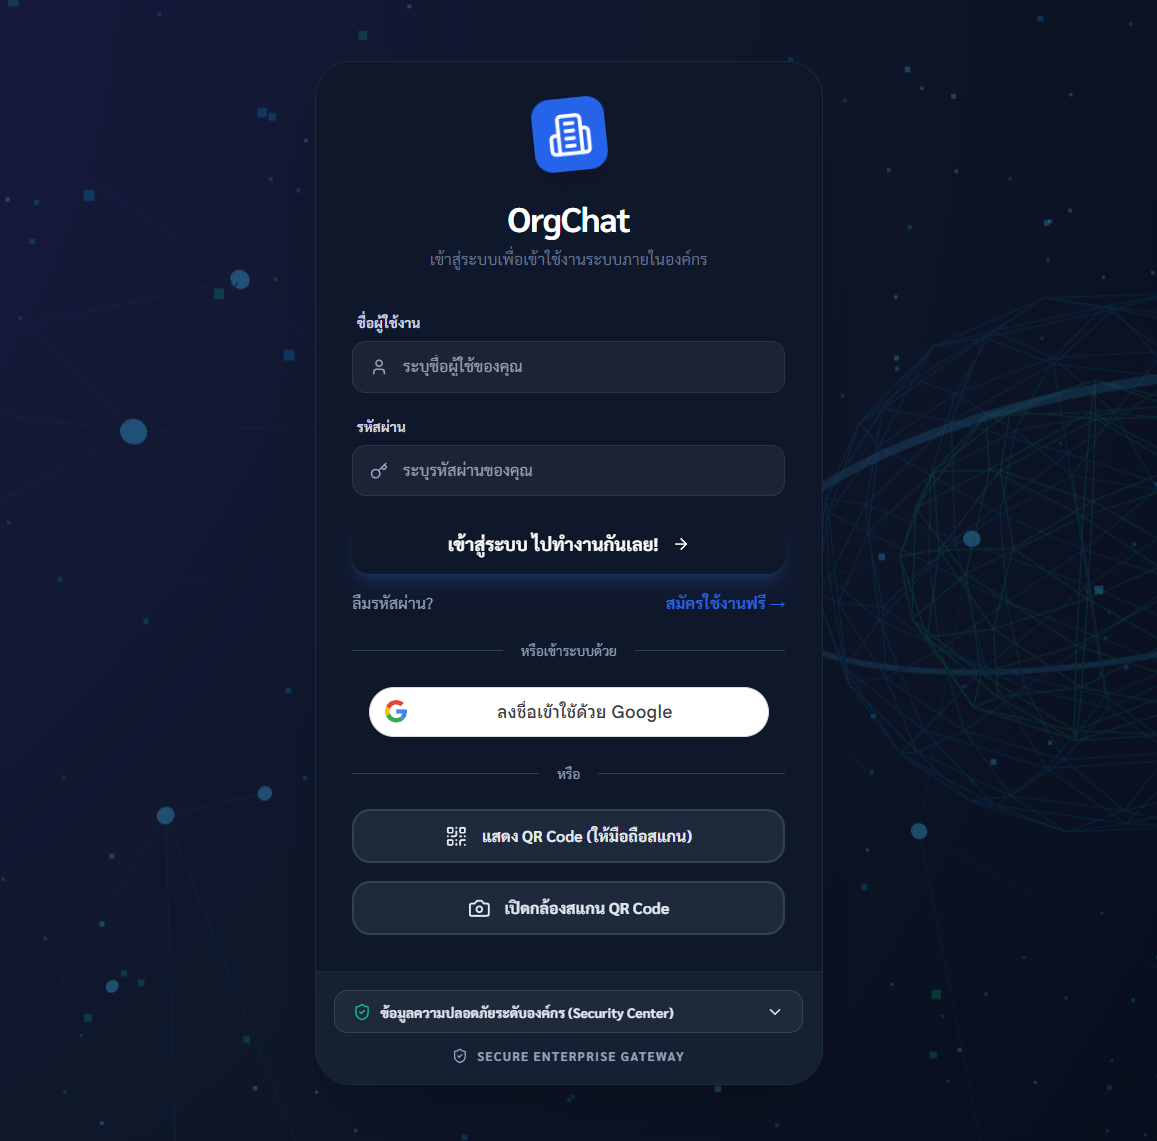
\includegraphics[width=0.88\textwidth]{Image/fig4_1_login.png}
\caption{หน้าจอเข้าสู่ระบบและสมัครสมาชิก OrgChat AI}
\label{figB:login}
\end{figure}

\subsection{การจัดการคลังความรู้องค์กร (Knowledge Base Management)}
\hspace*{1.3em}
ผู้ดูแลระบบสามารถจัดการเอกสารความรู้และคู่มือสินค้าของบริษัท ฮาร์ทวอมมิ่ง จำกัด เพื่อให้ AI สามารถนำไปใช้ตอบคำถามพนักงานได้ โดยมีขั้นตอนดังนี้:
\begin{enumerate}[leftmargin=3.5em]
\item \textbf{การเข้าสู่หน้าคลังความรู้}: เลือกเมนู "คลังความรู้ (Knowledge Base)" จากแถบเมนูด้านซ้ายของระบบเว็บแอปพลิเคชัน ดังแสดงในภาพที่ ข-2
\item \textbf{การอัปโหลดเอกสารใหม่}: 
  \begin{itemize}[leftmargin=2em]
    \item คลิกที่บริเวณพื้นที่อัปโหลดไฟล์ หรือลากไฟล์เอกสาร (รองรับไฟล์นามสกุล .pdf, .txt, .csv) มาวางในกรอบ
    \item ระบบจะตรวจสอบความถูกต้องของไฟล์ คำนวณค่าแฮช SHA-256 เพื่อตรวจจับไฟล์ซ้ำ และแสดงแถบความคืบหน้าของการอัปโหลด
    \item ระบบส่งไฟล์ไปจัดเก็บและสำรองไว้บนโฟลเดอร์ Google Drive ขององค์กรโดยอัตโนมัติ
  \end{itemize}
\item \textbf{กระบวนการประมวลผลเวกเตอร์ (Vector Indexing)}: ระบบจะทำการสกัดข้อความ ตัดแบ่งท่อนข้อมูล (Chunking) และแปลงเป็นเวกเตอร์เอ็มเบดดิงบันทึกลงสู่ ChromaDB สถานะเอกสารจะเปลี่ยนเป็น "พร้อมใช้งาน (READY)"
\item \textbf{การจัดการเอกสารเดิม}: ผู้ดูแลระบบสามารถตรวจสอบรายชื่อเอกสาร วันที่อัปโหลด ขนาดไฟล์ จำนวนท่อนข้อมูล (Chunks) และสามารถกดปุ่ม "ลบเอกสาร" เพื่อนำข้อมูลออกจากฐานข้อมูลเวกเตอร์ได้ทันที
\end{enumerate}

\begin{figure}[htbp]
\centering
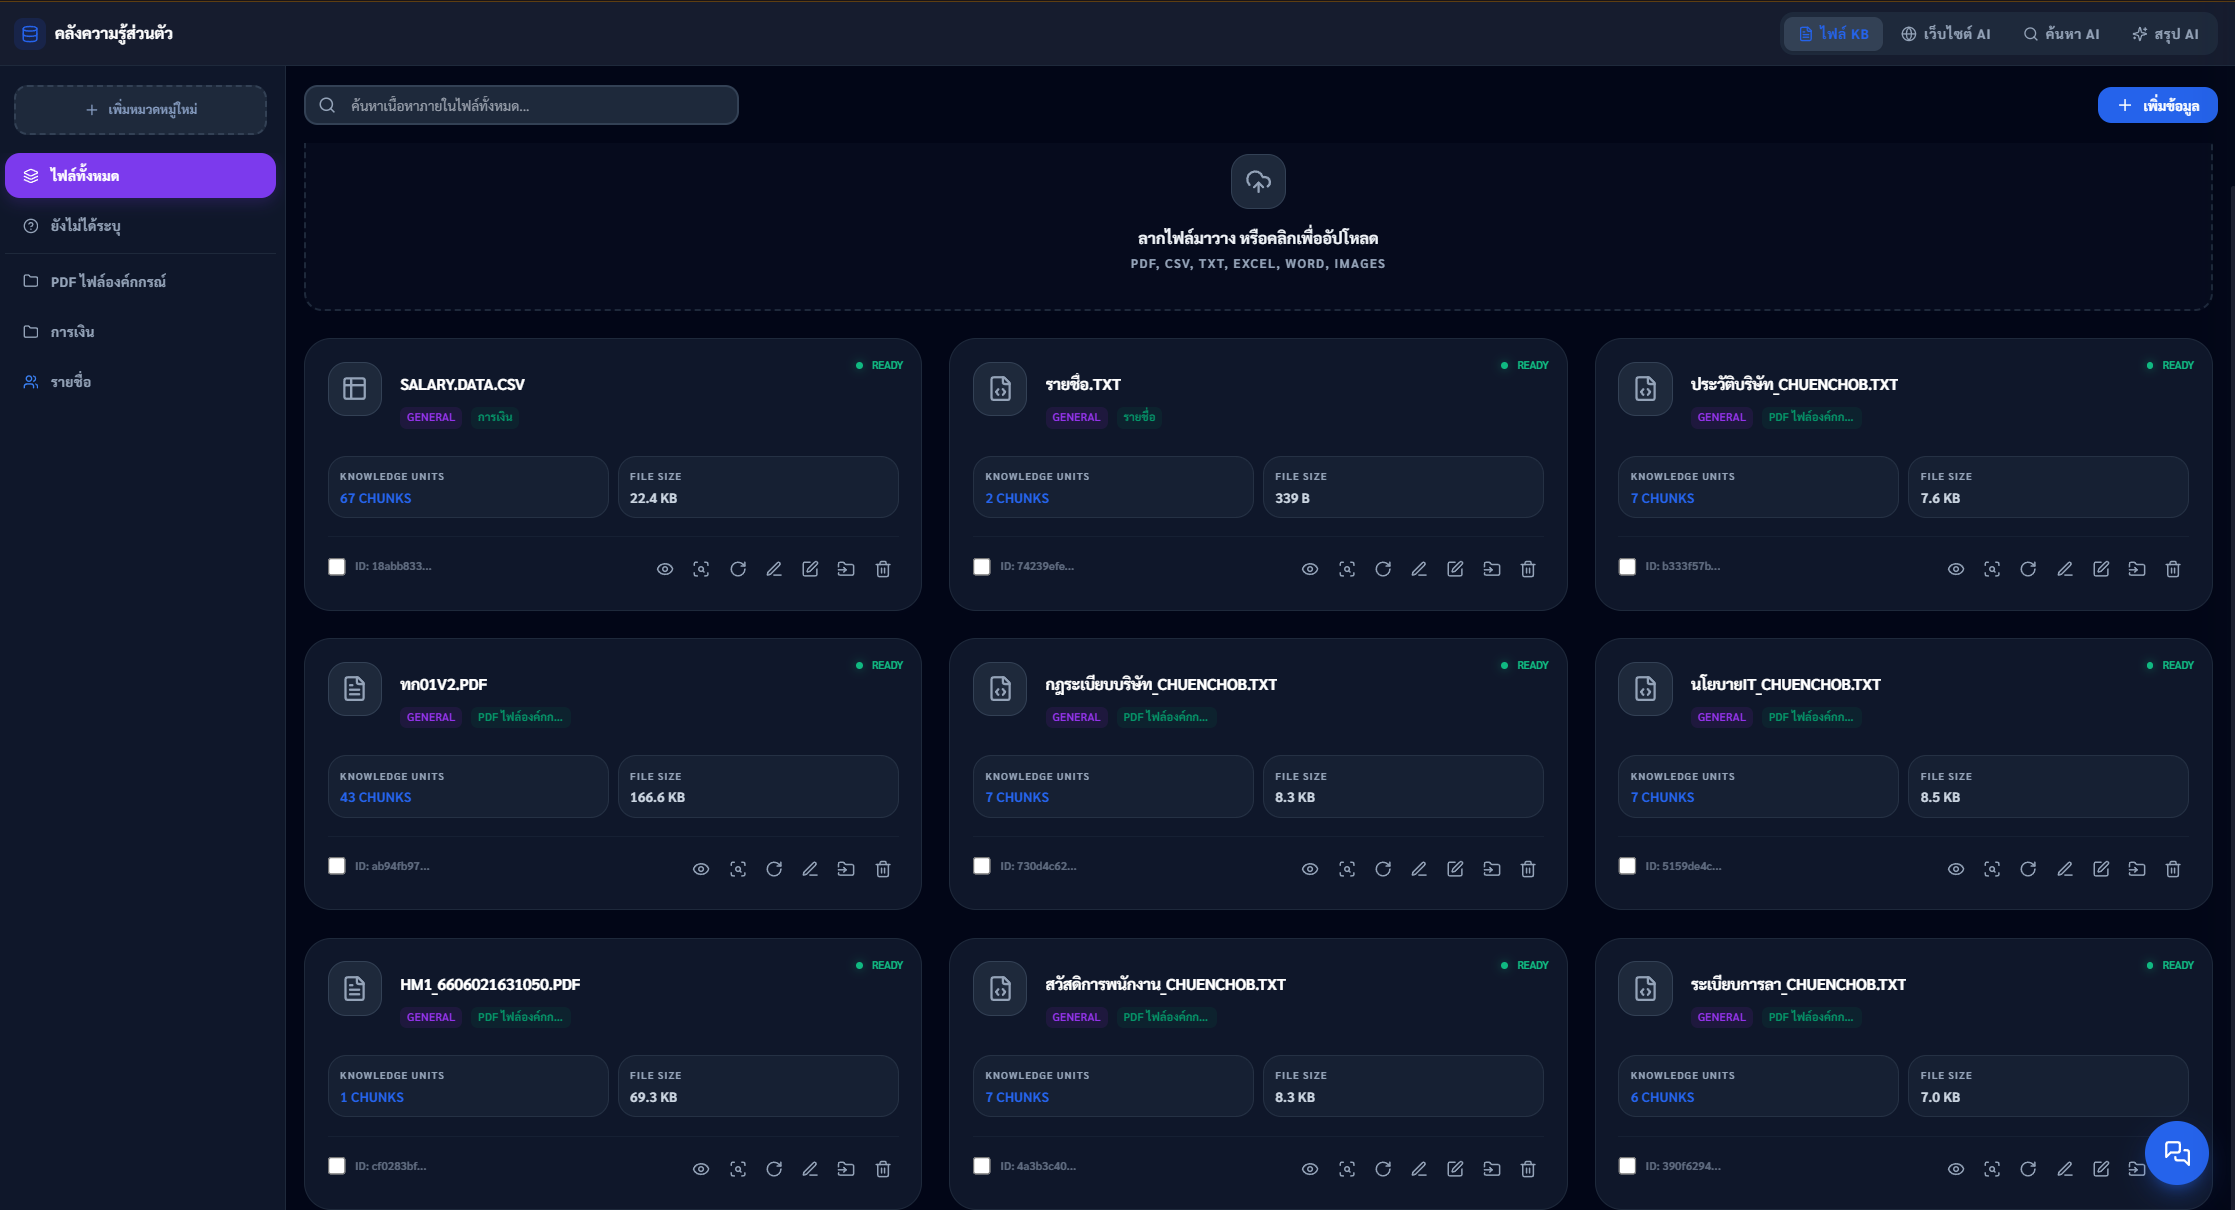
\includegraphics[width=0.88\textwidth]{Image/fig4_3_rag_kb.png}
\caption{หน้าจอการจัดการคลังความรู้องค์กรและการอัปโหลดเอกสาร}
\label{figB:rag_kb}
\end{figure}

\newpage
\subsection{การใช้งานแชทบอทผ่าน LINE Official Account (LINE Bot Interaction)}
\hspace*{1.3em}
พนักงานของบริษัท ฮาร์ทวอมมิ่ง จำกัด สามารถใช้งานผู้ช่วยอัจฉริยะในการสอบถามข้อมูลสินค้าและระเบียบปฏิบัติได้ทุกที่ทุกเวลาผ่านแอปพลิเคชัน LINE โดยมีขั้นตอนการใช้งานดังนี้:
\begin{enumerate}[leftmargin=3.5em]
\item \textbf{การเพิ่มเพื่อน}: สแกน QR Code หรือค้นหา LINE ID ของบัญชี LINE Official Account ของบริษัท และกดยืนยันการเพิ่มเพื่อน
\item \textbf{การพิมพ์คำถามภาษาธรรมชาติ}: พนักงานพิมพ์คำถามที่ต้องการทราบลงในช่องแชท เช่น \emph{"เงื่อนไขการรับประกันน้ำพุแมว duit เป็นอย่างไร"} หรือ \emph{"ถุงเท้าพิลาทิส thumb toe มีขนาดอะไรบ้าง"} ดังแสดงในภาพที่ ข-3
\item \textbf{การรับคำตอบจากแชทบอท}: ระบบจะค้นหาข้อมูลที่ตรงกันจากคลังความรู้และตอบกลับในรูปแบบการ์ด LINE Flex Message ที่จัดวางข้อความอย่างชัดเจน พร้อมแสดงแหล่งที่มาของเอกสารอ้างอิง
\item \textbf{การกดดูรายละเอียดเพิ่มเติม}: พนักงานสามารถกดปุ่มบนการ์ด Flex Message เพื่อเปิดดูเอกสารคู่มือฉบับเต็มบน Google Drive ได้โดยตรง
\end{enumerate}

\begin{figure}[htbp]
\centering

\includegraphics[height=0.42\textheight,keepaspectratio]{Image/fig4_2_line_rag.png}
\caption{การสนทนาสอบถามข้อมูลสินค้าผ่าน LINE Official Account}
\label{figB:line_rag}
\end{figure}

\subsection{การตรวจสอบประวัติการทำงานของระบบ (Audit Logs Inspection)}
\hspace*{1.3em}
ผู้ดูแลระบบสามารถตรวจสอบความโปร่งใสและความปลอดภัยของการใช้งานระบบ ผ่านหน้าจอบันทึกประวัติกิจกรรม (Audit Logs) ดังแสดงในภาพที่ ข-4:
\begin{enumerate}[leftmargin=3.5em]
\item เลือกเมนู "บันทึกกิจกรรม (Audit Logs)" จากแถบการนำทาง
\item ระบบจะแสดงตารางประวัติกิจกรรม ประกอบด้วย วันที่และเวลา, บัญชีผู้ใช้งาน, หมายเลข IP Address, ประเภทกิจกรรม (เช่น LOGIN, UPLOAD\_DOCUMENT, DELETE\_DOCUMENT) และสถานะผลลัพธ์
\item มีแถบค้นหาและตัวกรองตามช่วงเวลาและประเภทกิจกรรม เพื่อช่วยให้ผู้ดูแลระบบสามารถตรวจสอบความผิดปกติได้อย่างรวดเร็ว
\end{enumerate}

\begin{figure}[htbp]
\centering
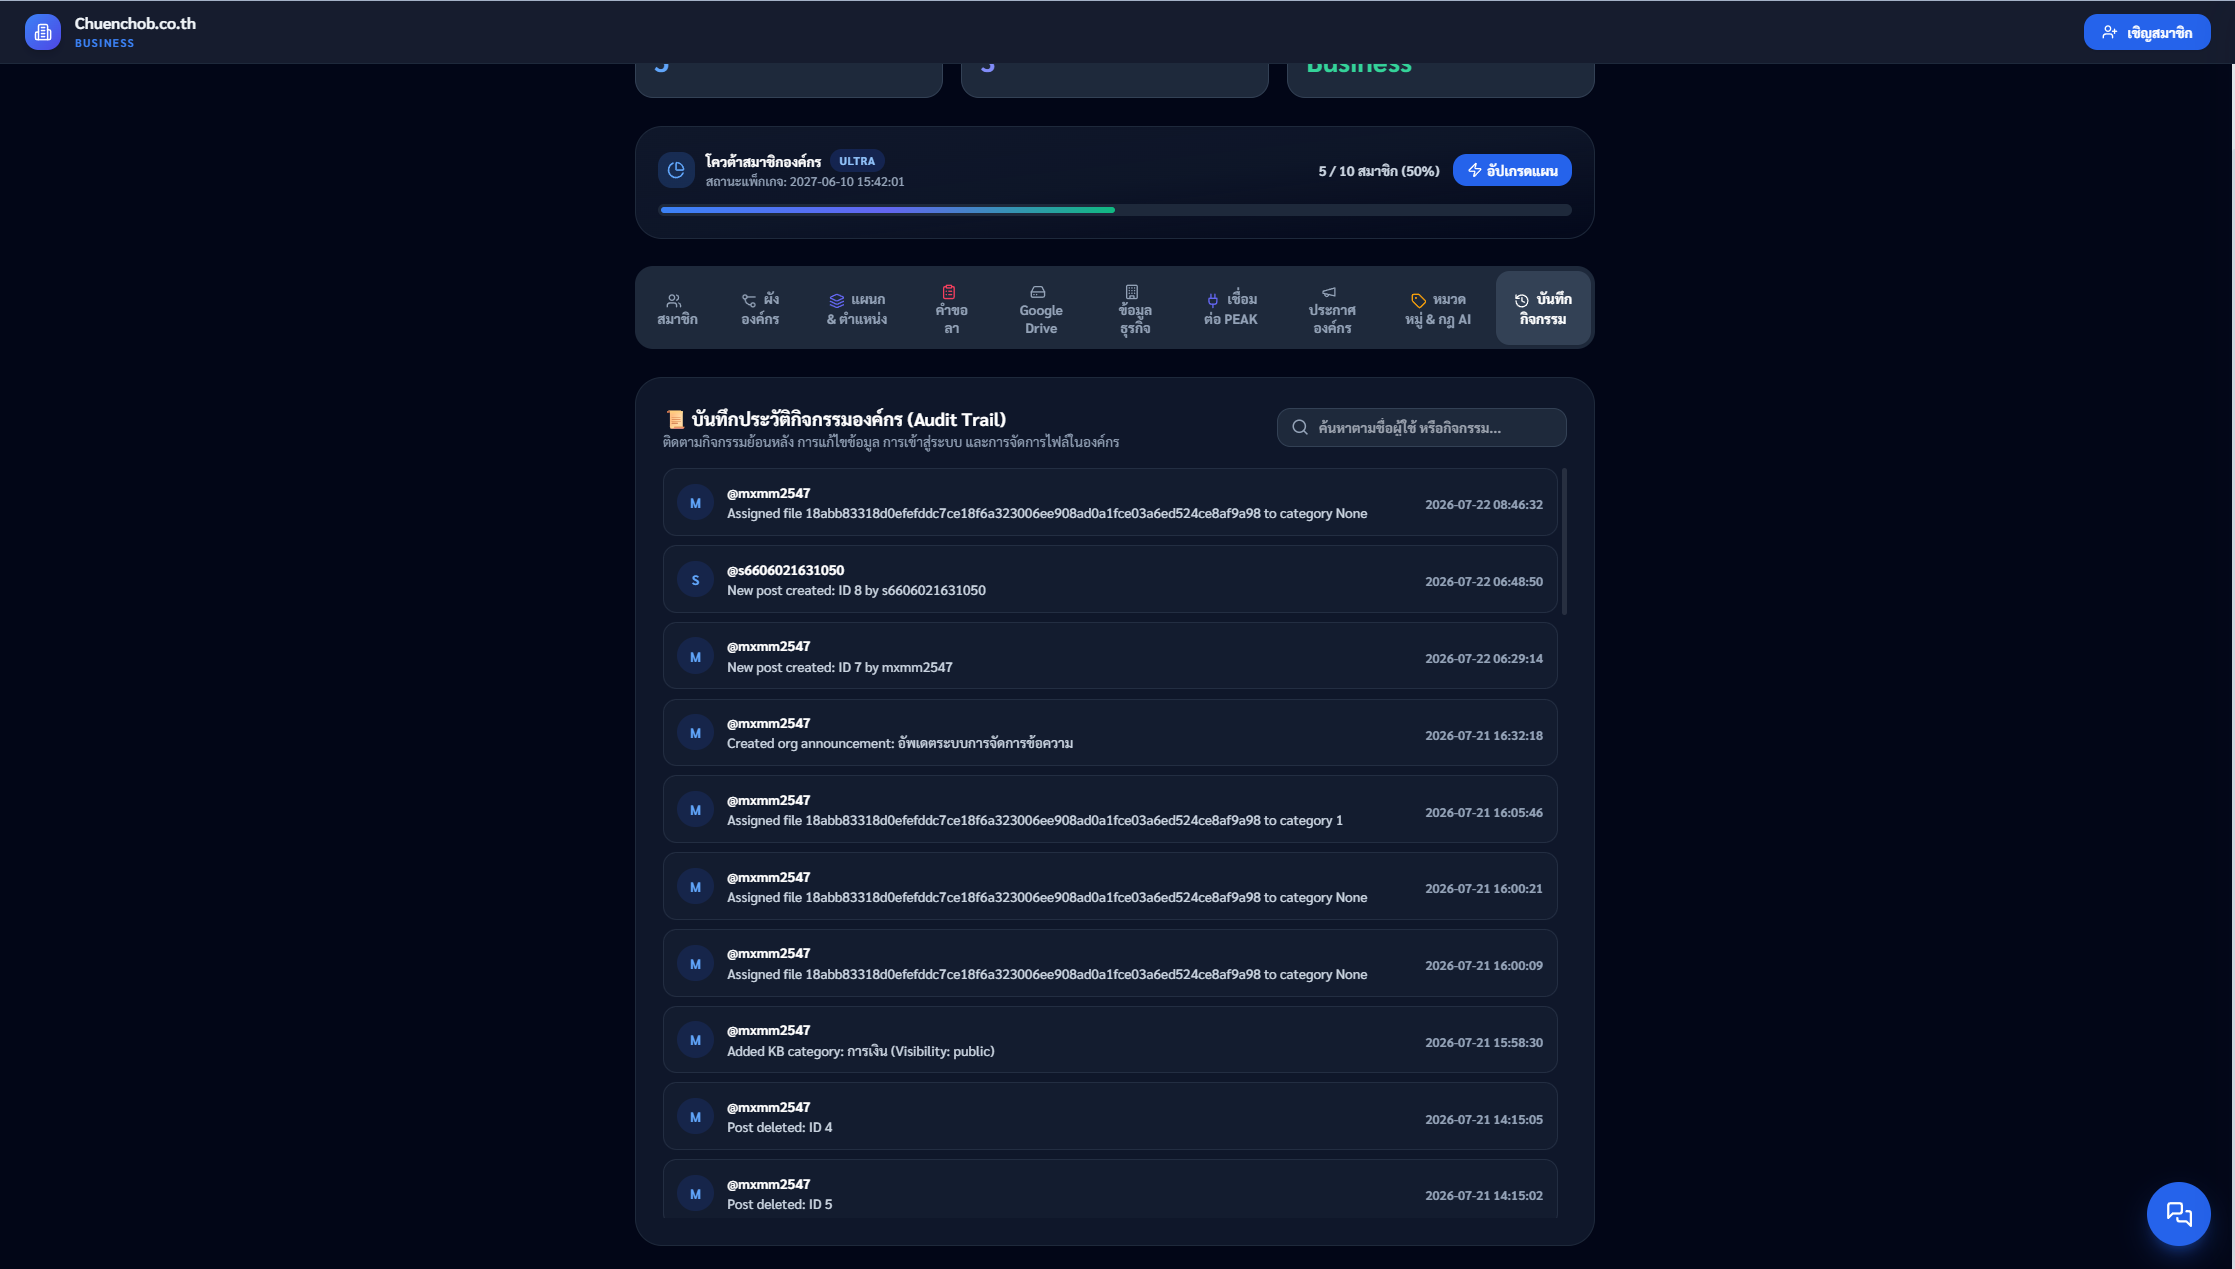
\includegraphics[width=0.88\textwidth]{Image/fig4_9_audit.png}
\caption{หน้าจอบันทึกประวัติการทำงานของระบบ (Audit Logs)}
\label{figB:audit}
\end{figure}

\newpage
\section{แบบร่างเครื่องมือประเมินความพึงพอใจสำหรับการดำเนินงานในภาคการศึกษาที่ 2/2569}
\hspace*{1.3em}
ในภาคการศึกษาที่ 2/2569 คณะผู้จัดทำมีแผนการนำระบบที่พัฒนาเสร็จสมบูรณ์ไปติดตั้งและทดสอบการใช้งานจริงร่วมกับบุคลากรของ บริษัท ฮาร์ทวอมมิ่ง จำกัด จำนวน 20 คน โดยจะใช้แบบสอบถามวัดความพึงพอใจตามมาตราส่วนประเมินค่า 5 ระดับของ Likert (Likert 5-Point Rating Scale) ซึ่งมีรายละเอียดของแบบร่างเครื่องมือดังแสดงในตารางที่ ข-1:

\vspace{0.5em}
\hspace*{1.3em}
\textbf{คำชี้แจง}: โปรดทำเครื่องหมาย $\checkmark$ ลงในช่องที่ตรงกับระดับความคิดเห็นของท่าน (5 = มากที่สุด, 4 = มาก, 3 = ปานกลาง, 2 = น้อย, 1 = น้อยที่สุด)

\begin{table}[htbp]
\centering
\caption{แบบร่างแบบสอบถามประเมินความพึงพอใจของผู้ใช้งานในภาคการศึกษาที่ 2/2569}
\label{tabB:survey}
\begin{tabularx}{\textwidth}{| c | L | c | c | c | c | c |}
\hline
\textbf{ข้อ} & \textbf{รายการประเมินความพึงพอใจ} & \textbf{5} & \textbf{4} & \textbf{3} & \textbf{2} & \textbf{1} \\ \hline
\multicolumn{7}{|l|}{\textbf{ด้านการออกแบบและการเข้าใช้งาน (Design and Usability)}} \\ \hline
1 & ความสะดวกและรวดเร็วในการเข้าใช้งานระบบผ่านแอปพลิเคชัน LINE & & & & & \\ \hline
2 & ความสวยงามและความชัดเจนของข้อความตอบกลับ LINE Flex Message & & & & & \\ \hline
3 & ความง่ายในการใช้งานหน้าจอเว็บแอปพลิเคชันสำหรับผู้ดูแลระบบ & & & & & \\ \hline
\multicolumn{7}{|l|}{\textbf{ด้านฟังก์ชันการทำงานและความถูกต้อง (Functionality and Accuracy)}} \\ \hline
4 & ความถูกต้องและตรงประเด็นในการตอบคำถามของระบบ RAG จากเอกสารคู่มือสินค้า & & & & & \\ \hline
5 & ความแม่นยำในการอ่านและสกัดข้อมูลจากภาพถ่ายสลิปโอนเงินด้วย OCR & & & & & \\ \hline
6 & ความสะดวกในขั้นตอนการยื่นคำขอลางานและการอนุมัติใบลาผ่าน LINE & & & & & \\ \hline
7 & ความครบถ้วนและประโยชน์ของข้อมูลสถิติบนแผงควบคุมผู้บริหาร (Dashboard) & & & & & \\ \hline
\multicolumn{7}{|l|}{\textbf{ด้านประโยชน์และความพึงพอใจในภาพรวม (Overall Benefits)}} \\ \hline
8 & ระบบช่วยลดระยะเวลาและขั้นตอนในการทำงานประจำวันของพนักงาน & & & & & \\ \hline
9 & ระบบช่วยลดข้อผิดพลาดในการรวบรวมข้อมูลและการสื่อสารภายในองค์กร & & & & & \\ \hline
10 & ความพึงพอใจในภาพรวมต่อการนำระบบ OrgChat AI มาช่วยปฏิบัติงาน & & & & & \\ \hline
\end{tabularx}
\end{table}

\newpage
\section{ประวัติผู้จัดทำโครงงาน (Author Biographies)}
\vspace{0.5em}

\subsection{นายธนากร ธนบวรพล (Mr. Thanakorn Thanabowonphon)}
\begin{mycustomitem}
\item \textbf{รหัสนักศึกษา}: 66-060-216-10117
\item \textbf{วัน เดือน ปีเกิด}: 15 กรกฎาคม พ.ศ. 2546
\item \textbf{สาขาวิชา}: สาขาวิชาเทคโนโลยีสารสนเทศ ภาควิชาเทคโนโลยีสารสนเทศ
\item \textbf{คณะ}: คณะเทคโนโลยีและการจัดการอุตสาหกรรม มหาวิทยาลัยเทคโนโลยีพระจอมเกล้าพระนครเหนือ (วิทยาเขตปราจีนบุรี)
\item \textbf{ประวัติการศึกษา}:
  \begin{itemize}[leftmargin=2em,noitemsep,topsep=2pt]
    \item พ.ศ. 2565: สำเร็จการศึกษาระดับมัธยมศึกษาตอนปลาย แผนการเรียนวิทยาศาสตร์-คณิตศาสตร์
    \item พ.ศ. 2566--ปัจจุบัน: กำลังศึกษาระดับปริญญาตรี หลักสูตรวิทยาศาสตรบัณฑิต สาขาวิชาเทคโนโลยีสารสนเทศ คณะเทคโนโลยีและการจัดการอุตสาหกรรม มจพ. ปราจีนบุรี
  \end{itemize}
\item \textbf{หน้าที่ความรับผิดชอบในโครงงาน}:
  \begin{itemize}[leftmargin=2em,noitemsep,topsep=2pt]
    \item วิเคราะห์และออกแบบระบบงานตามความต้องการของ บริษัท ฮาร์ทวอมมิ่ง จำกัด
    \item ออกแบบแผนภาพระบบ แผนภาพกระแสข้อมูล (DFD Level 0-2) และสถาปัตยกรรมระบบ
    \item ออกแบบแบบจำลองความสัมพันธ์ของข้อมูล (ER Diagram) และโครงสร้างตารางฐานข้อมูล SQLite
    \item พัฒนาระบบยืนยันตัวตน (Authentication) และระบบควบคุมสิทธิ์ตามบทบาท (RBAC)
    \item ออกแบบและเชื่อมต่อบริการ Google Drive API สำหรับจัดเก็บเอกสารองค์กร
    \item จัดทำเอกสารข้อกำหนดระบบ พจนานุกรมข้อมูล และจัดทำรายงานปริญญานิพนธ์
  \end{itemize}
\end{mycustomitem}

\newpage
\subsection{นายวีรภัทร ชื่นชอบ (Mr. Weeraphat Chuenchob)}
\begin{mycustomitem}
\item \textbf{รหัสนักศึกษา}: 66-060-216-31050
\item \textbf{วัน เดือน ปีเกิด}: 24 กันยายน พ.ศ. 2546
\item \textbf{สาขาวิชา}: สาขาวิชาเทคโนโลยีสารสนเทศ ภาควิชาเทคโนโลยีสารสนเทศ
\item \textbf{คณะ}: คณะเทคโนโลยีและการจัดการอุตสาหกรรม มหาวิทยาลัยเทคโนโลยีพระจอมเกล้าพระนครเหนือ (วิทยาเขตปราจีนบุรี)
\item \textbf{ประวัติการศึกษา}:
  \begin{itemize}[leftmargin=2em,noitemsep,topsep=2pt]
    \item พ.ศ. 2565: สำเร็จการศึกษาระดับมัธยมศึกษาตอนปลาย แผนการเรียนวิทยาศาสตร์-คณิตศาสตร์
    \item พ.ศ. 2566--ปัจจุบัน: กำลังศึกษาระดับปริญญาตรี หลักสูตรวิทยาศาสตรบัณฑิต สาขาวิชาเทคโนโลยีสารสนเทศ คณะเทคโนโลยีและการจัดการอุตสาหกรรม มจพ. ปราจีนบุรี
  \end{itemize}
\item \textbf{หน้าที่ความรับผิดชอบในโครงงาน}:
  \begin{itemize}[leftmargin=2em,noitemsep,topsep=2pt]
    \item ศึกษา วิจัย และพัฒนาระบบคลังความรู้อัจฉริยะ (RAG Pipeline) ด้วย ChromaDB และ FastEmbed
    \item พัฒนาระบบตัดแบ่งท่อนข้อมูล (Text Chunking) และสกัดข้อมูลจากเอกสารคู่มือสินค้า
    \item เชื่อมต่อและปรับแต่งโมเดล Google Gemini 1.5 Flash API สำหรับสังเคราะห์คำตอบภาษาธรรมชาติ
    \item พัฒนาระบบแชทบอท LINE Official Account ผ่าน LINE Messaging API Webhook
    \item ออกแบบและพัฒนาการแสดงผลข้อมูลด้วยการ์ด LINE Flex Message แบบ Interactive
    \item ดำเนินการทดสอบการทำงานของระบบ (Functional Black-Box Testing) และบันทึกผลการดำเนินงาน
  \end{itemize}
\end{mycustomitem}


\end{document}
